%%%%%%%%%%%%%%%%%%%%%%%%%%%%%%%%%%%%%%%%%
% kaobook
% LaTeX Template
% Version 1.3 (December 9, 2021)
%
% This template originates from:
% https://www.LaTeXTemplates.com
%
% For the latest template development version and to make contributions:
% https://github.com/fmarotta/kaobook
%
% Authors:
% Federico Marotta (federicomarotta@mail.com)
% Based on the doctoral thesis of Ken Arroyo Ohori (https://3d.bk.tudelft.nl/ken/en)
% and on the Tufte-LaTeX class.
% Modified for LaTeX Templates by Vel (vel@latextemplates.com)
%
% License:
% CC0 1.0 Universal (see included MANIFEST.md file)
%
%%%%%%%%%%%%%%%%%%%%%%%%%%%%%%%%%%%%%%%%%

%----------------------------------------------------------------------------------------
%	PACKAGES AND OTHER DOCUMENT CONFIGURATIONS
%----------------------------------------------------------------------------------------

\documentclass[
	a4paper, % Page size
	fontsize=10pt, % Base font size
	twoside=true, % Use different layouts for even and odd pages (in particular, if twoside=true, the margin column will be always on the outside)
	%open=any, % If twoside=true, uncomment this to force new chapters to start on any page, not only on right (odd) pages
	%chapterentrydots=true, % Uncomment to output dots from the chapter name to the page number in the table of contents
	numbers=noenddot, % Comment to output dots after chapter numbers; the most common values for this option are: enddot, noenddot and auto (see the KOMAScript documentation for an in-depth explanation)
]{kaobook}

% Choose the language
\ifxetexorluatex
	\usepackage{polyglossia}
	\setmainlanguage{english}
\else
	\usepackage[english]{babel} % Load characters and hyphenation
\fi
\usepackage[english=british]{csquotes}	% English quotes

% Load packages for testing
\usepackage{blindtext}
%\usepackage{showframe} % Uncomment to show boxes around the text area, margin, header and footer
%\usepackage{showlabels} % Uncomment to output the content of \label commands to the document where they are used

% Load the bibliography package
\usepackage{kaobiblio}
\addbibresource{main.bib} % Bibliography file

% Load mathematical packages for theorems and related environments
\usepackage[framed=true]{kaotheorems}

% Load the package for hyperreferences
\usepackage{kaorefs}

\graphicspath{{examples/documentation/images/}{images/}} % Paths in which to look for images

\makeindex[columns=3, title=Alphabetical Index, intoc] % Make LaTeX produce the files required to compile the index

\makeglossaries % Make LaTeX produce the files required to compile the glossary
\newglossaryentry{computer}{
	name=computer,
	description={is a programmable machine that receives input, stores and manipulates data, and provides output in a useful format}
}

% Glossary entries (used in text with e.g. \acrfull{fpsLabel} or \acrshort{fpsLabel})
\newacronym[longplural={Frames per Second}]{fpsLabel}{FPS}{Frame per Second}
\newacronym[longplural={Tables of Contents}]{tocLabel}{TOC}{Table of Contents}

 % Include the glossary definitions

\makenomenclature % Make LaTeX produce the files required to compile the nomenclature

% Reset sidenote counter at chapters
%\counterwithin*{sidenote}{chapter}

%----------------------------------------------------------------------------------------

\begin{document}

%----------------------------------------------------------------------------------------
%	BOOK INFORMATION
%----------------------------------------------------------------------------------------

% \titlehead{The \texttt{kaobook} class}
% \subject{Use this document as a template}

\title[Distributed edge cloud architecture for executing AI based applications]{Distributed edge cloud architecture for executing AI based applications}
% \subtitle{Customise this page according to your needs}

\author[Youssouph FAYE]{Youssouph FAYE}

\date{\today}

\publishers{Université Savoie Mont Blanc}

%----------------------------------------------------------------------------------------

\frontmatter % Denotes the start of the pre-document content, uses roman numerals

%----------------------------------------------------------------------------------------
%	OPENING PAGE
%----------------------------------------------------------------------------------------

%\makeatletter
%\extratitle{
%	% In the title page, the title is vspaced by 9.5\baselineskip
%	\vspace*{9\baselineskip}
%	\vspace*{\parskip}
%	\begin{center}
%		% In the title page, \huge is set after the komafont for title
%		\usekomafont{title}\huge\@title
%	\end{center}
%}
%\makeatother

%----------------------------------------------------------------------------------------
%	COPYRIGHT PAGE
%----------------------------------------------------------------------------------------

% \makeatletter
% \uppertitleback{\@titlehead} % Header

% \lowertitleback{
% 	\textbf{Disclaimer}\\
% 	You can edit this page to suit your needs. For instance, here we have a no copyright statement, a colophon and some other information. This page is based on the corresponding page of Ken Arroyo Ohori's thesis, with minimal changes.
	
% 	\medskip
	
% 	\textbf{No copyright}\\
% 	\cczero\ This book is released into the public domain using the CC0 code. To the extent possible under law, I waive all copyright and related or neighbouring rights to this work.
	
% 	To view a copy of the CC0 code, visit: \\\url{http://creativecommons.org/publicdomain/zero/1.0/}
	
% 	\medskip
	
% 	\textbf{Colophon} \\
% 	This document was typeset with the help of \href{https://sourceforge.net/projects/koma-script/}{\KOMAScript} and \href{https://www.latex-project.org/}{\LaTeX} using the \href{https://github.com/fmarotta/kaobook/}{kaobook} class.
	
% 	The source code of this book is available at:\\\url{https://github.com/fmarotta/kaobook}
	
% 	(You are welcome to contribute!)
	
% 	\medskip
	
% 	\textbf{Publisher} \\
% 	First printed in May 2019 by \@publishers
% }
% \makeatother

%----------------------------------------------------------------------------------------
%	DEDICATION
%----------------------------------------------------------------------------------------

\dedication{
	The harmony of the world is made manifest in Form and Number, and the heart and soul and all the poetry of Natural Philosophy are embodied in the concept of mathematical beauty.\\
	\flushright -- D'Arcy Wentworth Thompson
}

%----------------------------------------------------------------------------------------
%	OUTPUT TITLE PAGE AND PREVIOUS
%----------------------------------------------------------------------------------------

% Note that \maketitle outputs the pages before here

\maketitle

%----------------------------------------------------------------------------------------
%	PREFACE
%----------------------------------------------------------------------------------------

\chapter*{Preface}
\addcontentsline{toc}{chapter}{Preface} % Add the preface to the table of contents as a chapter

I am of the opinion that every \LaTeX\xspace geek, at least once during 
his life, feels the need to create his or her own class: this is what 
happened to me and here is the result, which, however, should be seen as 
a work still in progress. Actually, this class is not completely 
original, but it is a blend of all the best ideas that I have found in a 
number of guides, tutorials, blogs and tex.stackexchange.com posts. In 
particular, the main ideas come from two sources:

\begin{itemize}
	\item \href{https://3d.bk.tudelft.nl/ken/en/}{Ken Arroyo Ohori}'s 
	\href{https://3d.bk.tudelft.nl/ken/en/nl/ken/en/2016/04/17/a-1.5-column-layout-in-latex.html}{Doctoral 
	Thesis}, which served, with the author's permission, as a backbone 
	for the implementation of this class;
	\item The 
		\href{https://github.com/Tufte-LaTeX/tufte-latex}{Tufte-Latex 
			Class}, which was a model for the style.
\end{itemize}

The first chapter of this book is introductory and covers the most
essential features of the class. Next, there is a bunch of chapters 
devoted to all the commands and environments that you may use in writing 
a book; in particular, it will be explained how to add notes, figures 
and tables, and references. The second part deals with the page layout 
and design, as well as additional features like coloured boxes and 
theorem environments.

I started writing this class as an experiment, and as such it should be 
regarded. Since it has always been intended for my personal use, it may
not be perfect but I find it quite satisfactory for the use I want to 
make of it. I share this work in the hope that someone might find here 
the inspiration for writing his or her own class.

\begin{flushright}
	\textit{Federico Marotta}
\end{flushright}

\index{preface}

% \chapter*{Acknowlegments}
% \chapter{Abstract}

% The rise of edge computing marks a pivotal shift in how data-intensive applications are deployed and scaled. By relocating computation closer to the data source, edge architectures offer a compelling solution to the latency and bandwidth constraints inherent in cloud-based systems. This shift is particularly transformative for live video analytics, where real-time responsiveness is critical across domains such as public safety, traffic management, and autonomous systems. Processing video streams locally enables faster decision-making and reduces the overhead of transmitting raw data to centralized servers. Yet, the promise of edge computing is tempered by its limitations—most notably, constrained computational resources and the complexity of managing dynamic workloads.

% Among the most promising yet challenging sources of video data are mobile cameras. Their ability to capture scenes from diverse and timely vantage points makes them invaluable for situational awareness. However, their unpredictable presence and constantly shifting perspectives introduce significant architectural challenges. Unlike fixed cameras, mobile feeds resist traditional background subtraction techniques and demand more resource-intensive models for object detection and tracking. Moreover, their intermittent connectivity and erratic data volumes undermine conventional workload balancing strategies, which rely on stable input patterns. To address these constraints, this thesis introduces VideoJam, a decentralized load balancing framework designed to adaptively distribute video processing tasks across edge nodes. By predicting short-term workload fluctuations and coordinating traffic offloading among neighboring components, VideoJam ensures low-latency performance and resilience to runtime changes—without requiring centralized control or static configurations.

% Beyond the challenge of managing video traffic, edge systems must also contend with the growing need to support multiple deep learning models simultaneously. As analytics pipelines become more complex, co-locating deep neural networks (DNNs) on shared GPUs is no longer optional—it is essential for maximizing limited resources and maintaining real-time performance. However, this necessity introduces a critical problem: interference at the GPU kernel level, where competing models can silently degrade each other's performance. Existing orchestration frameworks often overlook these low-level dynamics, resulting in unpredictable throughput and compromised service guarantees. To address this, the second contribution of this thesis presents Roomie, a kernel-aware orchestration system that profiles and anticipates interference patterns between co-deployed models. By leveraging these insights, Roomie enables intelligent placement decisions that preserve inference quality and ensure predictable behavior in resource-constrained edge environments.

% Together, VideoJam and Roomie form a cohesive response to the evolving demands of edge-based video analytics. This thesis not only advances the technical foundations of decentralized load balancing and model orchestration, but also reimagines how edge systems can remain agile, scalable, and intelligent in the face of dynamic data sources and constrained hardware. Through these contributions, it lays the groundwork for next-generation edge architectures capable of supporting real-time, high-fidelity analytics across heterogeneous environments.

% =========


Edge computing has emerged as a transformative paradigm for real-time video analytics, offering low-latency processing by relocating computation closer to data sources. This shift is especially critical in domains such as public safety, traffic management, and autonomous systems, where responsiveness and bandwidth efficiency are crucial. Yet, edge environments are inherently resource-constrained and must contend with dynamic workloads, particularly when incorporating mobile cameras. These cameras provide valuable, timely perspectives but introduce unpredictability in data volume and scene composition, challenging traditional analytics pipelines and static workload distribution strategies. To address these constraints, this thesis presents \textit{VideoJam}, a decentralized load balancing framework that predicts short-term workload fluctuations and redistributes video traffic across edge nodes, enabling adaptive, low-latency performance without centralized coordination.

As edge systems evolve to support increasingly diverse AI tasks, a second challenge arises, one that lies not in data flow but in model deployment. Indeed, colocating multiple deep neural networks (DNNs) on shared GPUs has become a practical necessity, driven by the need to maximize limited computing resources while maintaining real-time inference. However, this necessity poses a fundamental challenge because when multiple models share the same hardware, their simultaneous execution can lead to competition for limited resources, resulting in slower performance and reduced reliability in meeting application requirements. Existing orchestration frameworks tend to adopt reactive or coarse-grained strategies, often neglecting the nuanced interactions that occur during model execution. To address this, this thesis introduces \textit{Roomie}, a kernel-aware orchestration system that profiles and anticipates interference between co-deployed models, enabling insightful placement decisions that preserve throughput and ensure consistent performance in resource-constrained deployments.

Together, these contributions advance the design of scalable, adaptive edge architectures capable of supporting high-fidelity video analytics across heterogeneous and dynamic deployments.


%----------------------------------------------------------------------------------------
%	TABLE OF CONTENTS & LIST OF FIGURES/TABLES
%----------------------------------------------------------------------------------------

\begingroup % Local scope for the following commands

% Define the style for the TOC, LOF, and LOT
%\setstretch{1} % Uncomment to modify line spacing in the ToC
%\hypersetup{linkcolor=blue} % Uncomment to set the colour of links in the ToC
\setlength{\textheight}{230\hscale} % Manually adjust the height of the ToC pages

% Turn on compatibility mode for the etoc package
\etocstandarddisplaystyle % "toc display" as if etoc was not loaded
\etocstandardlines % "toc lines" as if etoc was not loaded

\tableofcontents % Output the table of contents

\listoffigures % Output the list of figures

% Comment both of the following lines to have the LOF and the LOT on different pages
\let\cleardoublepage\bigskip
\let\clearpage\bigskip

\listoftables % Output the list of tables

\endgroup

%----------------------------------------------------------------------------------------
%	MAIN BODY
%----------------------------------------------------------------------------------------

\mainmatter % Denotes the start of the main document content, resets page numbering and uses arabic numbers
\setchapterstyle{kao} % Choose the default chapter heading style

\setchapterpreamble[u]{\margintoc}
\chapter{Introduction}
\labch{intro}

\section{Motivation}

% The rapid evolution of artificial intelligence over the past decade has transformed it from a research curiosity into a powerful force that is revolutionizing industries, societies, and our understanding of automation. This surge in AI applications, spanning domains such as video surveillance, healthcare diagnostics, autonomous systems, and real-time analytics, demands an infrastructure capable of handling vast computational workloads with speed and efficiency.

% A significant contributor to this demand is the increasing deployment of cameras used for safety, security, and traffic control applications. These cameras generate a massive amount of video data, which, when transmitted to centralized clouds for processing, poses substantial challenges in terms of bandwidth overheads. The sheer volume of data required to be transmitted and processed not only strains network resources but also leads to increased latency, making real-time analytics and response increasingly difficult.

% To address these challenges, there is a growing shift towards processing video streams at the edge, closer to where the data is generated. Edge devices, such as smart cameras and IoT devices, are being equipped with AI capabilities to analyze video streams in real-time, reducing the need for transmitting large volumes of data to centralized clouds. However, these edge devices typically have limited resources in terms of processing power, memory, and energy, posing significant constraints on the complexity and accuracy of AI models that can be deployed.

% The need for efficient AI infrastructure is thus becoming increasingly critical, driving innovations in edge computing, specialized hardware accelerators, and optimized AI algorithms. These advancements aim to enable the efficient deployment of AI at the edge, ensuring that the benefits of real-time video analytics can be realized without compromising on performance or resource utilization. Furthermore, the proliferation of mobile cameras, such as those mounted on cars, drones, and other vehicles, presents new opportunities for expanding the scope of video analytics. Equipped with high-quality camera sensors, these mobile cameras can provide unique perspectives and insights, often being in the right place at the right time to capture critical events. Integrating them into existing architectures will support a range of analytics applications that interest camera owners, such as accident detection, crash analytics, and reconstruction. However, the dynamic nature of mobile cameras, which capture scenes that vary more rapidly than those from fixed cameras, introduces new challenges in terms of data processing and analytics, underscoring the need for adaptable and robust AI models that can effectively handle these complexities.

% The integration of mobile cameras into video analytics systems presents several challenges, including the dynamic and unpredictable nature of the workload generated by these cameras. Specifically, the workload generated by mobile cameras is more dynamic and unpredictable, requiring constant adjustments to the processing infrastructure. Additionally, the continuously changing scenes captured by mobile cameras make customary processing pipelines ineffective, such as background subtraction, which works perfectly for fixed cameras but is ineffective for mobile cameras. Moreover, as mobile cameras appear and disappear from the deployment, they generate constant changes in the deployment configuration and the number of sources to process.

% As the scale and diversity of AI workloads grow, especially in video-centric environments, the challenge of distributing these workloads across available resources becomes increasingly important. We are entering a new era of workload distribution, where systems must adaptively allocate resources, balance latency constraints, and handle surges in demand. Effective workload distribution requires intelligent scheduling and resource awareness, taking into account the dynamic nature of mobile camera data and the need for real-time processing. By distributing workloads efficiently, systems can ensure that video analytics are performed in a timely and accurate manner, even in the presence of mobile cameras.

% In addition, the growing need to integrate AI functionality into edge devices and resource-constrained environments introduces additional challenges. In such contexts, colocating multiple AI models on shared hardware is often necessary to meet performance expectations. However, colocation introduces its own set of concerns, including resource contention, model interference, and degradation in quality-of-service metrics. The limited resources of edge devices make it essential to optimize the deployment of AI models, taking into account the risk of interference and conflicts between models.

% In this context, the use of specialized hardware accelerators such as graphics processing units (GPUs) can play a crucial role. Initially designed for complex graphics rendering in video games, the use of GPUs has become indispensable in modern AI systems. Their highly parallel architecture enables them to process massive datasets and run deep learning algorithms far more efficiently than traditional Central Processing Units (CPUs). Unlike CPUs, which excel in sequential task execution, GPUs can simultaneously execute thousands of threads making them particularly well-suited for training and inference workloads common in machine learning and deep neural networks (DNNs). Frameworks like Compute Unified Device Architecture (CUDA) and Open Computing Language (OpenCL) have further enhanced GPU utility by offering granular control over kernel execution, memory access, and thread parallelism. These APIs translate raw GPU power into scalable and optimized model deployment pipelines. CUDA, in particular, has become the de facto standard for programming NVIDIA GPUs, allowing researchers and engineers to harness low-level optimization capabilities and unlock breakthrough AI performance.

% To fully harness the potential of GPUs, it is essential to understand the underlying structure of these devices, including kernel scheduling and resource constraints. GPUs consist of multiple streaming multiprocessors, each with its own set of processing cores, registers, and shared memory. The efficient scheduling of GPU resources requires careful consideration of these constraints, including the management of register allocation, shared memory access, and warp scheduling. By optimizing GPU resource allocation and scheduling, it is possible to maximize the performance of AI workloads and ensure efficient processing of video analytics.

% Effective GPU scheduling in edge devices requires a deep understanding of the interplay between model characteristics, resource constraints, and performance objectives. This includes considering factors such as model complexity, input data rates, and latency requirements, as well as the available GPU resources, such as processing cores, memory, and bandwidth. By carefully balancing these factors, it is possible to develop scheduling strategies that optimize GPU utilization, minimize latency, and ensure efficient processing of video analytics workloads, even in power-constrained edge environments. Additionally, techniques such as dynamic voltage and frequency scaling, and power gating, can be employed to further optimize power consumption and performance.


% ---

% Edge computing is a transformative approach that brings computation and data storage closer to the data source, reducing latency and bandwidth usage. This proximity to the data source makes edge computing ideal for a wide range of applications, particularly those that require real-time processing and low latency, such as video analytics. Video analytics can be efficiently represented as pipelines of functions, where each function is an advanced algorithm or AI model that processes data and passes it to the next function, forming a Directed Acyclic Graph (DAG). This modular approach allows for scalable and flexible processing. However, deploying multiple models on the same device can lead to interference and degraded performance. Therefore, smartly distributing these models across available resources, taking into account their computational requirements and dependencies, can significantly enhance overall system performance and efficiency.

\subsection{The Evolution of Video Analytics and the Need for Edge Computing}

The proliferation of video streams has revolutionized various fields, from navigation and security to control systems, by providing an indispensable source of information. Whether it's monitoring traffic for efficient navigation, enhancing security through surveillance, or controlling industrial processes, video streams offer real-time insights that drive decision-making and automation. However, the exponential growth in data volume has made cloud-based processing increasingly impractical. The limitations of bandwidth and latency, coupled with the dependence on centralized resources, create significant bottlenecks. These issues make it difficult to process video data in real-time, leading to delays and inefficiencies.

This has driven a shift towards edge computing, which brings processing closer to the data source. By moving computation to the edge, we can reduce latency, conserve bandwidth, and improve the overall responsiveness of video analytics systems. Edge computing offers numerous benefits, but it also presents unique challenges, particularly in terms of resource constraints. Even with powerful GPUs, resources are not unlimited, compelling us to rethink traditional deployment strategies and workload distribution.

\subsection{Optimizing Resource Utilization in Edge Computing}

Optimizing resource utilization in edge computing environments, such as mobile platforms, low-power nodes, or remote devices, requires a modular approach to AI deployment. Decoupling the processing pipeline into separate functions (e.g., background subtraction, object detection, tracking, and classification), as in live video analytics, allows each stage to process data independently and pass results downstream, providing greater flexibility and efficiency. However, due to the limited computing and energy resources available in these environments, colocating multiple AI models on shared hardware often becomes a necessity to meet real-time performance requirements and reduce deployment costs. This pragmatic choice, while effective in theory, introduces a series of challenges: resource contention, interference between models, and degradation of quality of service metrics. Existing solutions often overlook these dynamics, deploying entire pipelines on single devices or distributing them without considering the negative interactions between co-deployed models. To mitigate these risks and ensure fair, predictable, and high-performance AI inference, sophisticated planning and optimization strategies are essential.

A fundamental first step in this process is to recognize and measure interference between co-deployed models before assigning them to a target GPU resource. By doing so, we can strategically deploy functions across available resources, maximizing the efficiency of edge devices. This requires a good understanding of how the GPU execution model works during inference. Such an understanding hinges on grasping the internal mechanics of GPU architecture. Designed to manage intensive workloads, GPUs rely on a highly parallel structure made up of multiple streaming multiprocessors, each with its own set of processing cores, registers, and shared memory. This configuration enables GPUs to excel at the training and inference tasks central to machine learning and deep neural networks (DNNs).

Frameworks like Compute Unified Device Architecture (CUDA) and Open Computing Language (OpenCL) have enhanced GPU utility by offering granular control over kernel execution, memory access, and thread parallelism. CUDA, in particular, has become the standard for programming NVIDIA GPUs, enabling researchers and engineers to harness low-level optimization capabilities and achieve breakthrough AI performance. However, understanding how kernels are scheduled and executed in the GPU during inference is crucial. Once deployed, each model will execute several kernels successively. Moreover, every kernel requires a certain amount of register allocation, shared memory, and warps to run efficiently. This low-level view complements high-level planning strategies, enabling smarter placement of models, particularly in edge environments where resource constraints necessitate the co-deployment of deep neural networks (DNNs).

\subsection{Addressing Fluctuating Workloads and Mobile Cameras}

Beyond the complexities of deployment, the performance of video analytics systems is often limited by fluctuations in workload from camera sources, due to the constant evolution of captured scenes over time. Since the number and nature of objects in images vary (e.g., sudden crowd formation or vehicle movements), different functions in the processing pipeline (e.g., object detection, tracking, and classification) experience uneven computational loads, leading to temporal imbalance and resource conflicts across the system. These temporal imbalances in data generation can cause certain nodes to be overloaded while leaving others underutilized, potentially leading to data gaps and diminished analytical precision. To address this issue, recent research has explored distribution strategies, either by vertically offloading excess traffic between edge devices and centralized cloud resources, or by horizontally distributing workloads across edge clusters. However, such strategies implicitly rely on the predictability and stability of video input, typically generated from fixed cameras with consistent monitoring patterns.

This assumption begins to break down with the emergence of mobile cameras. Unlike their fixed counterparts, mobile cameras offer advantages such as increased coverage, dynamic perspectives, and enhanced situational awareness. Yet, they also introduce distinct challenges—most notably, the rapid and unpredictable variation in scene content. This volatility disrupts traditional workload planning and demands adaptive processing strategies that can respond in real-time to fluctuating video streams and computational needs.

This thesis aims to introduce and design an innovative architecture tailored to the aforementioned challenges associated with deploying video analytics applications in resource-constrained environments. The proposed framework will establish efficient methods for distributing and managing processing pipelines to adapt to fluctuating workloads. By optimizing resource efficiency and streamlining task distribution, we will be able to improve the overall performance and reliability of video analytics systems in varied and constantly evolving scenarios.

\section{Contributions of this Thesis}

This thesis makes several key contributions to the field of edge computing and video analytics:

Self-Balancing Architecture for Live Video Analytics: VideoJam implements a distributed load balancing system by deploying load balancers colocated with each task in the analytics pipeline. Each load balancer continuously monitors the incoming flow of frames or objects and periodically shares this information with neighboring load balancers. Based on the collected data, each load balancer independently decides how much traffic to process locally and whether to offload some of its workload to less-burdened neighbors using a lightweight machine learning model that predicts the incoming workload for each processing component and its neighbors in the near future. Additionally, the load balancers employ a congestion prevention signaling system to correct any prediction errors. VideoJam operates autonomously, adapting dynamically to changes such as new camera arrivals or departures without requiring system reboots, and balances incoming traffic accordingly. Our approach uniquely combines horizontal distribution and per-function type load balancing, driven by short-term forecasts of incoming loads.

Efficient Model Cohabitation in Edge Computing Model Serving: an orchestration architecture designed to maximize system performance in scenarios where model colocation is necessary, particularly in resource-constrained edge environments. The key innovation of Roomie is its kernel-aware interference profiling, which captures the sequential nature of GPU kernel execution patterns when multiple models share hardware resources. By analyzing how specific kernel sequences from different models interact, Roomie constructs accurate interference profiles that predict performance degradation under various colocation scenarios. This detailed approach allows Roomie to make optimal placement decisions, determining which models can efficiently coexist on the same hardware and which combinations should be avoided to ensure performance guarantees.

Building upon these contributions, the next chapter (Chapter 2) will explore the foundational background and relevant literature that inform our research. This contextual groundwork is essential for grasping the significance of our innovations and the methodological choices made throughout the thesis, thereby enabling a holistic understanding of our strategy for optimizing edge computing and video analytics.

\setchapterpreamble[u]{\margintoc}
\chapter{Related work}\labch{related_work}


\section{Edge Computing and Video Analytics}
% \paragraph{The Evolution of Edge Computing Architectures.}

Edge computing represents a paradigm shift in distributed systems, wherein computational tasks and data storage are relocated closer to the data source. This architectural transformation addresses several limitations inherent in centralized cloud infrastructures, notably by reducing latency, minimizing bandwidth consumption, enhancing data security, and enabling real-time responsiveness. Given that edge devices, such as sensors, cameras, and Internet of Things (IoT) nodes, typically operate under constrained computational and energy resources, a variety of architectural models have emerged. These include hybrid edge-cloud systems, which balance local and remote processing, as well as fully autonomous edge analytics platforms designed for domain-specific applications, particularly within industrial IoT environments.

\paragraph{GPU Integration and Computational Enhancement.}
The incorporation of Graphics Processing Units (GPUs) into edge computing frameworks has significantly expanded the computational capabilities of edge systems. GPUs are inherently suited for parallel processing, rendering them ideal for compute-intensive tasks such as machine learning, computer vision, and large-scale data analytics. Their deployment at the edge yields notable improvements in performance, efficiency, and scalability. As a result, GPUs have become instrumental in enabling advanced edge applications, including autonomous vehicles, smart surveillance systems, immersive augmented and virtual reality (AR/VR) experiences, and responsive healthcare diagnostics. These applications benefit from the edge's capacity to process data locally and in real time, thereby reducing latency and enhancing decision-making accuracy. In industrial IoT contexts, for example, edge computing facilitates real-time monitoring and control of equipment, leading to increased operational efficiency and reduced downtime.

\paragraph{Video Analytics as a Critical Edge Application.}
Among the diverse applications of edge computing, video analytics emerges as a particularly demanding and impactful use case. In domains such as smart cities, autonomous driving, and public safety, edge-based video analytics enables the timely interpretation of visual data. A typical video analytics pipeline comprises several stages: data ingestion, preprocessing, feature extraction, model inference, and post-processing. Each stage imposes distinct computational and memory requirements, which are often challenging to satisfy within the limited capabilities of edge devices.

\paragraph{Resource Constraints and Architectural Challenges.}
The computational limitations of edge devices, manifested in restricted processing power, limited storage capacity, and constrained communication bandwidth, pose significant challenges to the deployment of complex video analytics workloads. These constraints necessitate the development of innovative strategies aimed at optimizing resource utilization while preserving the real-time performance and locality benefits of edge computing.

\paragraph{Optimization Strategies and Emerging Solutions.}
To address these challenges, researchers have proposed a spectrum of solutions designed to enhance performance without compromising the advantages of edge deployment. Techniques such as model compression and pruning have been employed to reduce the computational footprint of deep learning algorithms, thereby enabling their execution on resource-constrained devices. Distributed processing frameworks facilitate the partitioning and collaborative execution of workloads across multiple edge nodes, improving scalability and fault tolerance. Furthermore, adaptive scheduling algorithms and energy-aware resource management strategies have been developed to dynamically allocate tasks and balance performance with sustainability. Collectively, these approaches contribute to the realization of robust, efficient, and scalable edge computing systems capable of supporting increasingly complex and latency-sensitive applications.


\section{Load Balancing for Live Video Analytics}
% Load Balancing Techniques: Survey existing load balancing techniques for edge computing, with a focus on those relevant to video analytics. Discuss distributed load balancing approaches and the use of machine learning models in load balancing.

Recent advancements in video analytics have led to the development of various techniques aimed at enhancing application performance. These efforts span multiple dimensions, including architectural design, pipeline optimization, and data privacy. As the demand for real-time, scalable video processing grows, particularly in edge environments, thus efficient resource management and adaptability have become central challenges.

\paragraph{Video Analytics System Architecture.}
Early solutions focused on optimizing computational resources for video streams from fixed cameras. For example, Chameleon dynamically reconfigures pipeline placement to reduce resource consumption with minimal accuracy loss. Similarly, Spatula exploits spatial and temporal correlations among camera feeds to lower network and computation costs. However, these approaches are limited by their reliance on static camera inputs and do not address the complexities introduced by mobile video sources.

\paragraph{Deployment Strategies.}
To overcome the limitations of static architectures, newer frameworks have adopted distributed deployment models. Distream~\cite{zeng2020distream} exemplifies this shift by partitioning analytics pipelines between smart cameras and edge nodes, adapting to workload dynamics to maintain low latency and high throughput. The work presented in~\cite{} shows that the intelligent distribution and processing of vision modules in parallel on available peripheral computing nodes can ultimately enable better use of resources and improve performance. Likewise, VideoStorm~\cite{201465videostorm} which places different video functions across multiple available workers to satisfy users' requests. These strategies offer greater flexibility and scalability, making them more suitable for dynamic environments.

\paragraph{Load Balancing in Edge Video Analytics.}
As video analytics applications scale across distributed infrastructures, load balancing becomes essential for maintaining accuracy and low latency. Traditional methods, such as those used in VideoStorm~\cite{201465videostorm}, Spatula~\cite{jain2020spatula}, Hetero-edge~\cite{zhang2019hetero}, and VideoEdge~\cite{hung2018videoedge}, relied on static configurations and centralized cloud offloading. These approaches often resulted in network bottlenecks and were slow to adapt to changing workloads.
Recent developments have introduced more dynamic load balancing mechanisms. Distream, for example, offers pipeline-level load balancing that adapts to the variability of video content. However, its reliance on predictable long-term patterns such as daily traffic fluctuations limits its responsiveness to abrupt changes in video content or camera behavior.

\paragraph{Workload Prediction.}

To enhance load balancing, predictive models based on machine learning have been explored. Reinforcement learning, as used in~\cite{yuan2021online}, enables real-time task assignment but demands substantial computational resources and continuous training to mitigate concept drift. However, reinforcement learning solution, even though effective, require a significant amount of resources and continuous online training to avoid concept-drift problems~\cite{zhang2020reinforcement}. Linear regression models, as in~\cite{kombi2017preventive}, offer a simpler alternative but may lack the sophistication needed for complex scene dynamics.
Given the constraints of edge devices and the unpredictability of mobile camera inputs, there is a growing need for lightweight forecasting models. These models should be capable of short-term trend prediction, operate efficiently on resource-constrained hardware, and support real-time decision-making.


The evolution of video analytics has moved from static, centralized systems to dynamic, distributed architectures. While significant progress has been made in deployment and load balancing strategies, future research must focus on developing lightweight, adaptive forecasting techniques. These solutions should be tailored to the constraints of edge environments and the variability introduced by mobile video sources, ensuring scalable and responsive video analytics.


% In recent years, several techniques have been developed to improve the performance of video analytics applications~\cite{ibrahim2021survey,xu2023edge,hu2023edge}. Such a topic has been tackled from different perspectives, including the design of different data processing architectures~\cite{jain2020spatula,zhang2017live,jiang2018chameleon}, the improvement of pipelines' processing~\cite{fouladi2017encoding,chen2015glimpse,padmanabhan2021towards,padmanabhan2023gemel} and the privacy of the extracted data~\cite{cangialosi2022privid,poddar2020visor,wu2021pecam}.

% \paragraph{Architecture scaling.}
% Different approaches have been proposed to efficiently manage the computational resources for video analytics~\cite{jain2020spatula,zhang2017live,jiang2018chameleon,201465videostorm}. Chameleon, presented in~\cite{jiang2018chameleon}, frequently reconfigures the placement of video analytics pipelines to reduce resource consumption with small loss in accuracy. Another example is Spatula~\cite{jain2020spatula}, which exploits the spatial and temporal correlations among different camera flows to reduce the network and computation costs. However, such solutions only consider video flows coming from fixed cameras.

% \paragraph{Deployment strategies.} 
% Other solutions mainly focused on the deployment strategies of video analytics applications~\cite{zeng2020distream,201465videostorm,rachuri2021decentralized}. Distream~\cite{zeng2020distream} is a distributed framework based capable of adapting to workload dynamics to achieve low-latency, high-throughput and scalable live video analytics. Pipelines are deployed on both the smart cameras and the edge, and are jointly partitioned so that part is computed on the smart cameras, while the rest is sent towards the edge, which has more computing power at its disposal. The deployment of application pipelines is adapted to the varying processing load, however there is a lack of adaptability required by the rate of mobile cameras.
% The work in~\cite{rachuri2021decentralized} presents experimental results showing that smartly distributing and processing vision modules in parallel across available edge compute nodes, can ultimately lead to better resource utilization and improved performance. The same approach is also used by VideoStorm~\cite{201465videostorm} which places different video functions across multiple available workers to satisfy users' requests. We assume a deployment of pipelines in line with this latter work given the higher flexibility, higher scalability and the better use of resources of this approach. 

% \paragraph{Load balancing strategies.}
% Once video analytics applications have been deployed on a distributed edge infrastructure, load balancing strategies play a fundamental role in guaranteeing requirements of accuracy and efficiency. As a result, The concept of implementing load balancing for video analytics applications has gained popularity, particularly with the emergence of edge video analytics and its associated limitations. Historically, load balancing was performed between edge nodes and central clouds (\eg, VideoStorm~\cite{201465videostorm}), but this method became impractical due to increased network traffic and potential network bottlenecks. Load balancing between edge locations has been the subject of several works, including Spatula~\cite{jain2020spatula}, Hetero-edge~\cite{zhang2019hetero}, and VideoEdge~\cite{hung2018videoedge} (albeit VideoEdge still relies on offloading to remote clouds). However, these works focused on the production of static configurations, where each processed video is directed to a predetermined path through the deployed processing functions. As any change of configuration impacts the deployed functions, configuration updates occur over longer timescales, making these approaches unsuitable for highly variable loads. More recently, Distream~\cite{zeng2020distream} recognized the need for rapidly adapting to varying loads within a video, proposing an adaptable load balancing solution that splits the load balancing decisions at the pipeline level. However, it assumes that workflows present predictable longer-term patterns, allowing reconfiguration decisions only to be taken at longer timescales, for example when traffic conditions change during the day due to commute patterns.

% \paragraph{Workload prediction.}
% Workload predictions, based on machine learning models, have been proved to be effective in the design of load balancing policies~\cite{heinze2014auto,gedik2013elastic,kombi2017preventive,zeng2020distream}. In~\cite{yuan2021online}, authors used reinforcement learning for performing real-time estimation for dynamic assigning task to the optimal server. While the work in~\cite{kombi2017preventive}, focused on load forecasting by using linear regression model. However, reinforcement learning solution, even though effective, require a significant amount of resources and continuous online training to avoid concept-drift problems~\cite{zhang2020reinforcement}. Such a solution method is not suitable for the computational-constrained devices at the edge. In addition, the rapid changes in scenes captured by mobile cameras are more difficult to predict. Therefore, there is a need of lightweight forecasting models that can predict short-term trends, suitable for edge devices and fast enough for real-time prediction.



\section{Inference Serving and Resource Management in Edge Cloud Computing}

With the rise of deep learning applications deployed as online services, efficiently managing inference workloads in GPU datacenters has become a pressing concern. Unlike training tasks, inference jobs present unique constraints, requiring high accuracy, low latency, and cost-effectiveness. These goals often conflict, making it essential to design scheduling systems that can balance trade-offs without compromising overall performance.

\paragraph{Limitations of Early Serving Systems.}
Initial solutions such as Clipper~\cite{2017clipper} and TensorFlow-Serving focused on simplifying model deployment and supporting multiple frameworks. While they introduced dynamic scaling and model abstraction, they did not account for resource interference prior to deployment. Clockwork~\cite{gujarati2020servingdnnslikeclockwork} attempted to provide predictable performance by leveraging the deterministic nature of DNN inference under full GPU load. However, its design restricted execution to one inference at a time, resulting in underutilized GPU resources.

\paragraph{Multi-Tenant DNN Inference on Shared GPUs.}
A subsequent line of research investigates techniques for optimizing model performance in environments characterized by concurrent execution, where multiple models or processes must contend for shared GPU resources. This body of work typically examines scheduling algorithms, resource allocation strategies, and system-level adaptations designed to maintain throughput and minimize latency under constrained computational conditions. For example, Colti~\cite{} demonstrated that colocating DNN tasks can improve throughput. Another work proposed scheduling operators across dedicated CUDA streams, splitting execution into stages to balance concurrency and latency. Miriam introduced elastic kernels for edge GPUs, allowing dynamic remapping based on task priority. While these methods improve utilization, they operate reactively and do not explore optimal colocation strategies beforehand.

\paragraph{Interference-Aware Inference Serving.}
Recent studies have shifted toward proactive scheduling by modeling and predicting interference between concurrently running models. Some approaches estimate latency degradation using coarse features like buffer usage and PCIe traffic, but lack granularity. Scrooge~\cite{hu2021scrooge} profiles concurrency thresholds for identical models, though its scalability is limited by the number of possible combinations. Proteus~\cite{ahmad2024proteus} introduces adaptive batching and model variant selection to balance accuracy and latency, but its rigid placement strategy restricts colocation flexibility. These systems represent progress toward interference-aware scheduling, yet often rely on profiling techniques that are either too coarse or computationally intensive.

\paragraph{Fine-Grained GPU Scheduling for DNN Inference: Kernel-Level Insights and Limitations}
Recent approaches to GPU scheduling for deep neural network inference, such as iGniter~\cite{xu2022igniter} and Usher, emphasize low-level profiling to mitigate performance interference in shared environments. By analyzing metrics like core launches, cache usage, and kernel occupancy, these systems reveal that traditional coarse-grained models overlook critical scheduling dynamics. Usher further distinguishes between compute- and memory-intensive workloads, noting that large language models often strain memory bandwidth. Both rely on NVIDIA's Multi-Process Service (MPS)~\cite{} for resource partitioning, which limits their applicability on edge platforms lacking MPS support. This highlights the need for interference-aware strategies that operate independently of cloud-specific infrastructure.

The evolution of inference scheduling reflects a shift from general-purpose deployment tools to sophisticated, interference-aware systems. While early solutions prioritized ease of use, newer frameworks aim to anticipate and mitigate resource contention dynamically. However, we need a much fine-grained profiling, flexible model placement, and adaptive execution strategies to meet the complex demands of modern inference workloads.


\setchapterpreamble[u]{\margintoc}
\chapter{VideoJam: Self-Balancing Architecture for Live Video Analytics}
\labch{videojam}

% \section{Background and Motivation}
\section{Background and Motivation}
\label{sec:background_motivation}

In this section we present the characteristics of video analytics pipelines, providing motivation for integrating mobile video sources into the analytics architecture. We then present the key differences between fixed and mobile cameras, highlighting the challenges that we face when we integrate different types of cameras into such systems.

\subsection{Live Video Analytics}
% In this subsection we present the general characteristics of video analytics and types of choices we can take to make them function.

% \begin{figure}
%     \centering
%     \begin{subfigure}[t]{0.57\linewidth}
%         \centering
%         \includegraphics[width=\linewidth]{chapters/videojam/images/pipelines.pdf}
%         \caption{Applications use different modules depending on the source.}
%         \label{fig:pipelines}
%     \end{subfigure}
%     \hfill
%     \begin{subfigure}[t]{0.37\linewidth}
%         \centering
%         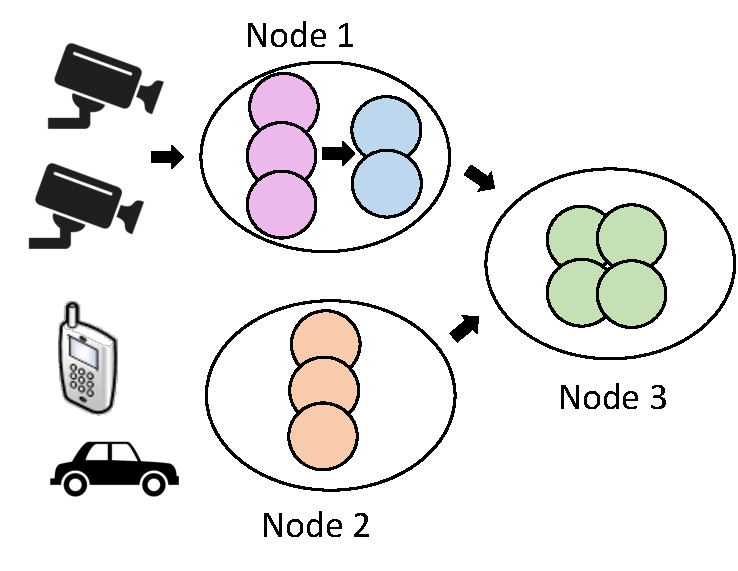
\includegraphics[width=0.8\linewidth]{chapters/videojam/images/dep_example.pdf}
%         \caption{The orchestration determines where to deploy replicas of each module.}
%         \label{fig:dep_example}
%     \end{subfigure}
%     \caption{The characteristics of live video analytics.\fb{I am not sure how needed this figure is or how to adapt it} \sj{The figure quality is quite poor as well.}}
%     \label{fig:video_analytics}
% \end{figure}

\begin{figure}[t]
    \centering
     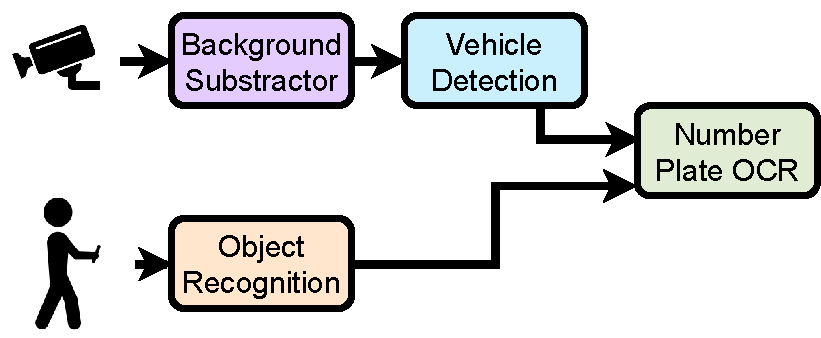
\includegraphics[width=0.75\linewidth]{chapters/videojam/images/video_analytics.pdf}
    \caption{The functions composing a vehicles' number plate detection application pipeline. Different sources require different processing functions.}
    \label{fig:video_analytics}
\end{figure}

% Paragraph on a high level description of video analytics and their applications
Live video analytics center around analyzing video camera streams in real-time, using algorithmic and computer vision techniques to extract valuable information. Incoming frames traverse a series of modules (or \textit{functions}) that perform different tasks, such as object detection, classification, and tracking. These functions are combined into a pipeline, conventionally represented by a directed acyclic graph, where the output of one function is the input of the next and the final output depends on the analytics application deployed.~\Cref{fig:video_analytics} shows an example of video analytics pipelines for a typical traffic control application: vehicles' number plate detection.

% Paragraph on the general structure of video analytics pipelines
Historically, video analytics research has focused its attention on the placement problem occurring at deployment time. Deploying a video analytics application involves taking an orchestration decision of where to place the instances of the application's pipeline. Placement decisions are taken based on the available resources in the compute infrastructure and the workload generated by available cameras. Early work on video analytics focused on how to efficiently transmit video traffic to centralized clouds for processing~\cite{ao2018sprocket,zhang2017live,fouladi2017encoding}. Yet, while centralized datacenters offer unbounded compute resources, transporting the increasing amounts of video streams to these locations can result in network bottlenecks, requiring either to preprocess video frames on premises~\cite{chen2015glimpse,hung2018videoedge} or to reduce the quality of the video transported~\cite{pakha2018reinventing}, potentially affecting the performance of deployed applications.

% Paragraph on the different choices we can take to make them function
To combat these challenges, recent work has focused on deploying video analytics pipelines at the edge of the network~\cite{zeng2020distream,jiang2018chameleon,zhang2019hetero}. These approaches aim to take advantage of compute resources deployed close to video cameras and bypass the transmission to remote locations. However, edge compute devices are often co-located with the existing network equipment and deploy limited computational resources. As a result, they can rapidly become overloaded by incoming video frames causing data loss and reduced accuracy. To address this challenge, different solutions have been proposed to distribute the workload across locations. For example, Distream~\cite{zeng2020distream} exploits the inherent load dynamics present in video flows to split the processing pipeline between two hierarchical locations, \ie, the camera and the edge compute machine. Chameleon~\cite{jiang2018chameleon} instead optimizes the pipelines configuration based on temporal and spatial predictions on the contents of camera sources. 

Yet, all these architectures assume that video flows are generated from fixed cameras (\eg, traffic cameras deployed at street corners) and that their workflows present predictable patterns allowing reconfiguration decisions to be taken at longer timescales, for example when traffic conditions change during the day due to commute patterns. However, mobile cameras have become pervasive in the last decade. Mobile devices, from smartphones to cars and drones all come equipped with high quality camera sensors. These cameras often have the unique advantage of being in the right place at the right time, offering the potential to enhance existing architectures and improve application performance. Unfortunately, video feeds generated by mobile cameras are fundamentally different from fixed camera ones, posing unique challenges into the path for their integration. 


\subsection{Challenges in Incorporating Mobile Cameras}

\begin{figure}
    \centering
    \begin{subfigure}[t]{0.47\linewidth}
        \centering
        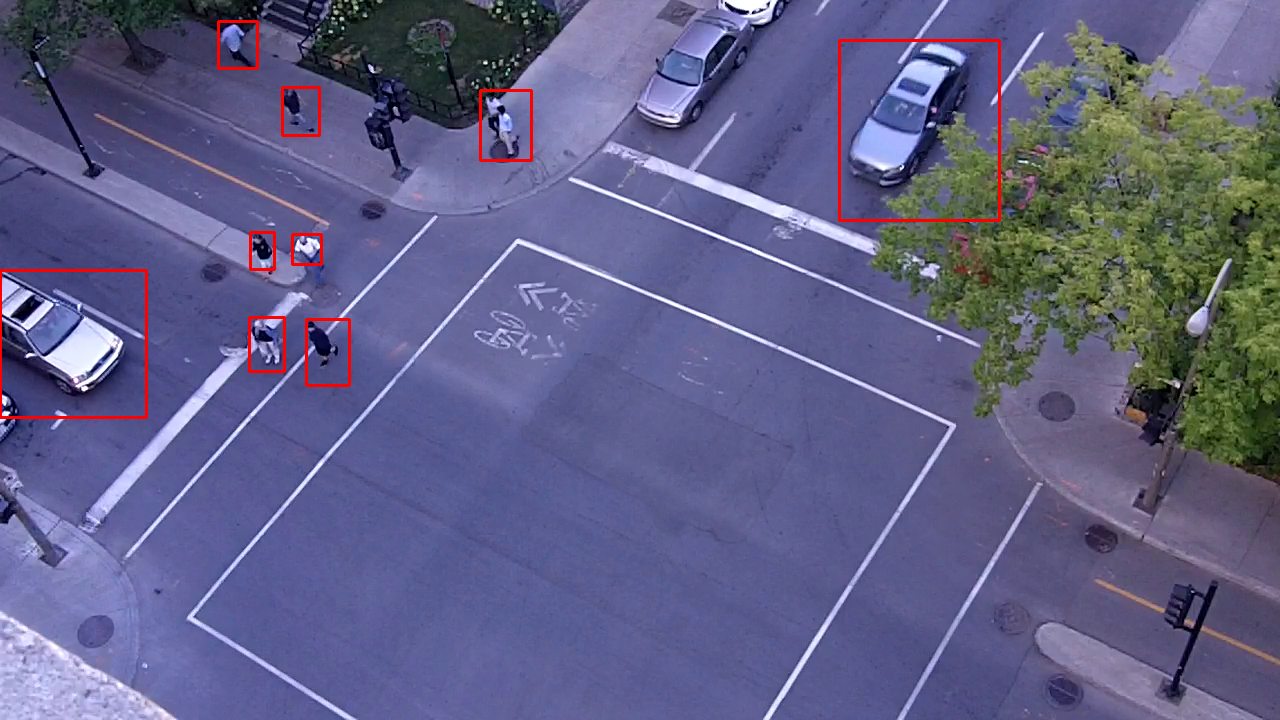
\includegraphics[width=\linewidth]{chapters/videojam/images/fixed_camera_bg_subtractor1003.png}
        \caption{Fixed camera with background subtractor.}
        \label{fig:fixed}
    \end{subfigure}
    \hfill
    \begin{subfigure}[t]{0.47\linewidth}
        \centering
        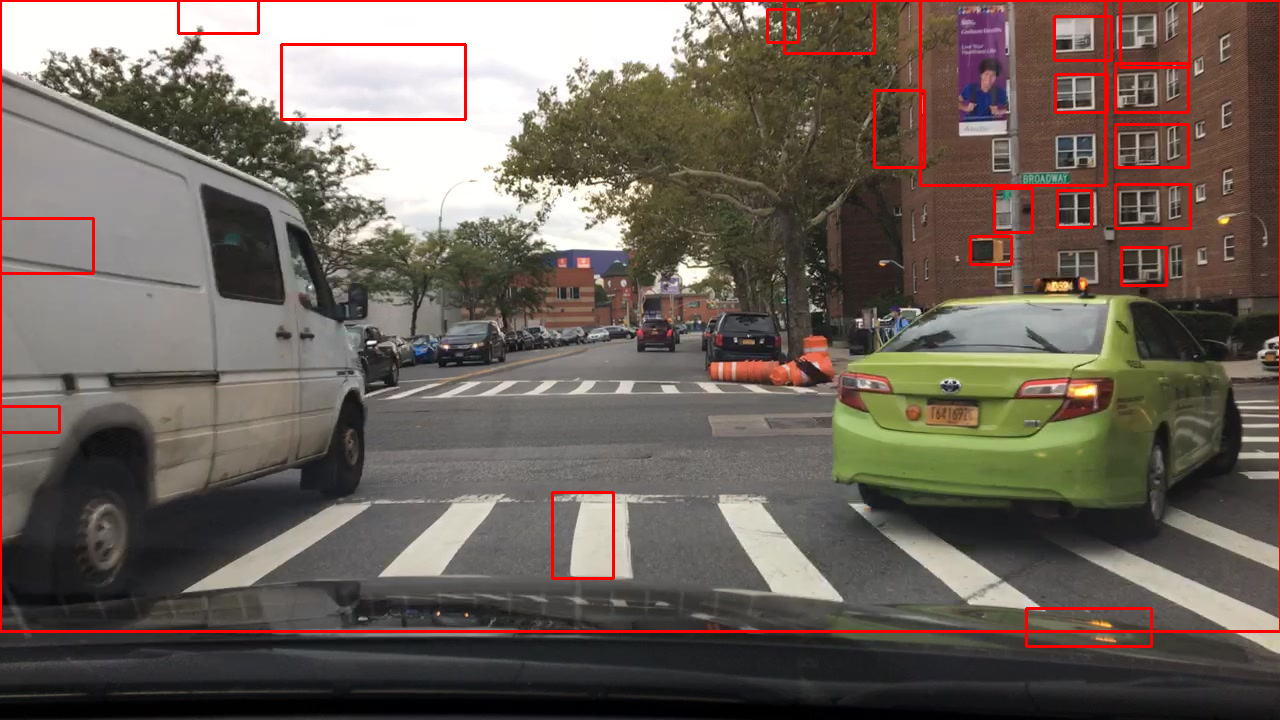
\includegraphics[width=\linewidth]{chapters/videojam/images/mobile_camera_bg_subtractor.png}
        \caption{Mobile camera with background subtractor.}
        \label{fig:mobile}
    \end{subfigure}
    \caption{A comparative example on the performance of background substractor functions on fixed and mobile cameras.}
    \label{fig:backgroung_subtractor}
\end{figure}


Mobile cameras bring the advantage of providing a unique perspective on the captured scenes. They can be in the right place at the right time, capturing scenes that would be otherwise invisible from fixed cameras. However, this benefit comes at the implicit cost of having to handle fundamentally different dynamics. Mobile cameras are constantly moving, capturing new scenes; they can appear and disappear from a deployment; and the scenes they capture can vary more rapidly than for fixed cameras. For these reasons, the differences between fixed and mobile cameras can greatly impact the deployment choices of a video analytics pipeline architecture that aims to process their video feeds. With the goal of designing a video analytics architecture that can handle both fixed and mobile cameras, we identify three core challenges that arise from the coexistence of these cameras in the same deployment.

%This discusses that while previous work uses traffic predict performance profiles, it is not enough to correctly balance the load in the presence of mobile cameras because they come and go.
\paragraph{Challenge \#1: Heterogeneous performance profiles.} 
The majority of existing video analytics solutions~\cite{jiang2018chameleon} assume the homogeneity in the performance of the processing components deployed. Distream~\cite{zeng2020distream} relaxes this assumption by considering the presence of heterogeneous processing devices and accounts for this disparity in implementing load balancing policies within its architecture. However, mobile cameras are inherently in constant movement, quickly capturing new scenes. This makes the processing pipelines that are effective for fixed cameras ineffective for mobile cameras.  

To exemplify the difference between fixed and mobile cameras, we consider a vehicles' number plate detection application. The goal of this application consists of detecting vehicles from a camera frame using a vehicle detection module and extract their number plate via an Optical Character Recognition (OCR) module. To lighten the load of the processing pipeline, the first step involves isolating objects in the frame to limit vehicle detection executions solely on cropped images~\cite{zeng2020distream}. This is typically done using a background subtractor module that compares the current frame with a background model and outputs a mask of the foreground objects~\cite{zeng2020distream}.~\Cref{fig:fixed} shows the output of a background subtractor module applied to a fixed camera frame. We observe that the background subtractor is able to isolate the moving objects in the frame while still objects (\eg, parked cars) are not detected as they are still in the frame. Unfortunately, while the application of a background subtractor is effective for fixed camera streams, the same pipeline becomes ineffective for mobile cameras. By nature, mobile cameras are constantly moving, capturing new scenes. As a consequence, when applied to a moving subject, the subtractor model is not capable of adapting to new scenes, causing erroneous detections or, in the worst case, detecting the entire frame as foreground (as shown in~\Cref{fig:mobile}).

% . shows
% the output of a background subtractor module applied to a mobile camera frame
% where the vehicles in the frame are not detected while other elements (\eg, the
% windows of the building) are. This makes it impossible to isolate the moving
% objects in the frame, forcing the deployment of more expensive object detection modules to process the entire frame. 

\begin{figure}
    \centering
    \begin{subfigure}[t]{0.47\linewidth}
        \centering
        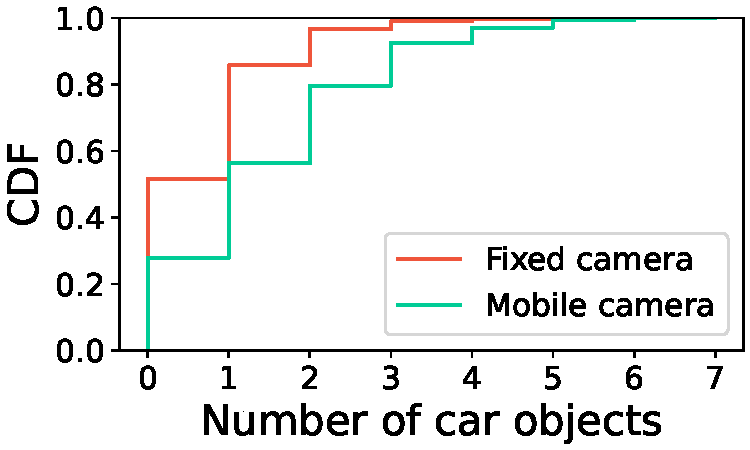
\includegraphics[width=\linewidth]{chapters/videojam/images/fixed_and_mobile_camera_output_filtered.pdf}
        \caption{Number of detected vehicles.}
    \end{subfigure}
    \hfill
    \begin{subfigure}[t]{0.47\linewidth}
        \centering
        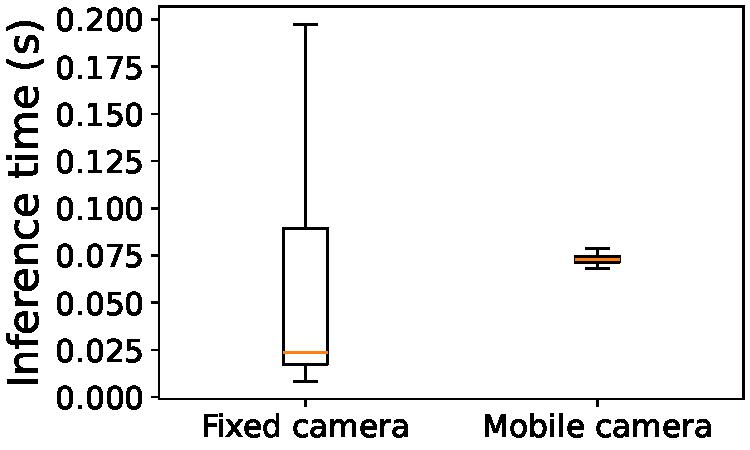
\includegraphics[width=\linewidth]{chapters/videojam/images/inference_times.pdf}
        \caption{Inference time.}
    \end{subfigure}
    \caption{Vehicle detection performance for fixed (background substractor + detection) vs mobile (YOLOv5) cameras.}
    \label{fig:mobile_v_fixed}
\end{figure}

To compensate for the degraded performance of the background substractor module, existing solutions tailored for mobile cameras~\cite{qiu2018kestrel,he2021real} replace the early stages of the pipeline with an object recognition module (\eg, YOLO~\cite{jocher2020yolov5}) that is capable of detecting and classifying objects in the frame in a single operation. However, this comes at a price, as detection models are more resource-intensive, especially for scenarios where no object is in the frame.~\Cref{fig:mobile_v_fixed} shows the performance difference between the two approaches on two selected videos, a fixed and mobile one. We observe that, while the number of detected vehicles is relatively similar across videos, the characteristics of the inference times for the two approaches highly varies depending on the processed frame. In fact, while YOLO achieves consistent results due to its single-pass nature, the performance of the combination of background subtractor and vehicle detection varies according to the number of vehicles present in the frame. Ultimately, this leads to the conclusion that the two approaches should not be treated as interchangeable and that the choice of the pipeline to deploy should be tailored to the video source type.

%This discusses the fact that while previous work aims to balance the load across clusters, it is not enough to balance the load, the presence of diverse pipelines requires different load balancing policies across difference locations.
\paragraph{Challenge \#2: Highly variable workloads.} 
Previous work has highlighted how video camera feeds differ in the amount of objects of interest they capture depending on their deployment location (\eg, a building entrance vs. an emergency exit) and the time of capture (\eg, at night vs during the day)~\cite{yildiz2013optimal,guo2021crossroi}. These differences generate variability in the workload that the video analytics pipeline needs to process and have been exploited to design more efficient processing pipelines~\cite{jiang2018chameleon,zeng2020distream}. Distream~\cite{zeng2020distream} proposed to exploit this variability to dynamically balance the workloads across processing clusters, taking advantage of periods of lower usage from some nodes in the architecture to support overloaded ones. Their solution achieves this through the use of two main design elements: (i) A cross-device workload balancer that takes the cross-camera workload correlations and the heterogeneous compute capabilities of smart cameras and edge clusters to optimize cross-camera workload balancing via an optimization problem; and (ii) a workload adaption controller which triggers the cross-camera workload balancer when cross-camera workload imbalance is detected. 

Unfortunately, this approach assumes that workloads have predictable profiles, either due to the cameras' relative locations, their time of capture~\cite{jiang2018chameleon}, or, more generally, by training a prediction model based on previous patterns~\cite{zeng2020distream}. However, the introduction of mobile cameras generates a new level of variability in the workload that is not easily predictable. First, mobile cameras constantly vary their point of observation and might capture different scenes at different instances in time. Second, the inherent moving nature of mobile cameras causes them to appear or disappear from the deployment, generating sudden changes in the workload that the video analytics pipeline needs to process. Overall, relying on long term prediction models to infer incoming load is not sufficient, or even potentially counter-productive, to correctly balance the load in the presence of mobile cameras.

\begin{figure}
    \centering
    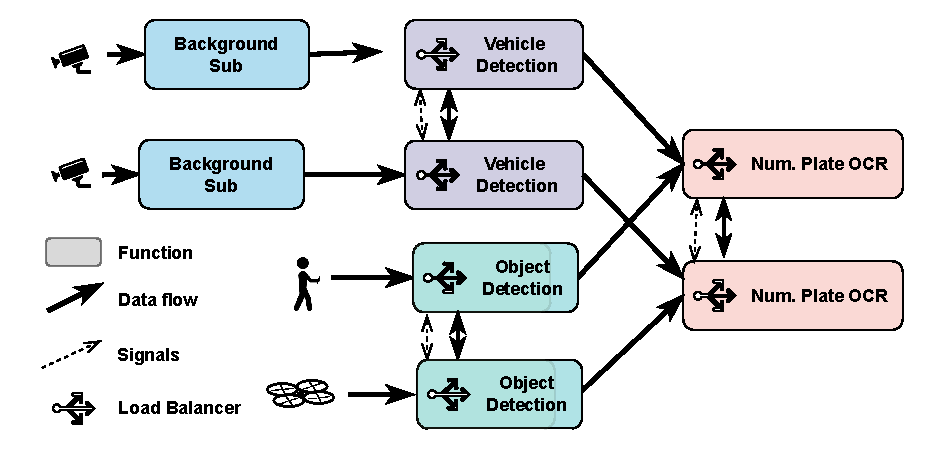
\includegraphics[width=\linewidth]{chapters/videojam/images/architecture.pdf}
    \caption{VideoJam architecture.}
    \label{fig:architecture}
\end{figure}

%This discusses how ultimately we can focus on the previous two, but if the configuration changes, we are screwed. We need an online approach. In particular, there can be a change in in number 
\paragraph{Challenge \#3: Varying configurations.} Early work in video analytics focused on the problem of optimizing the placement in the infrastructure of the functions that belong to the processing pipelines. The placement decisions behind this optimization are conventionally driven by the available resources in the compute infrastructure, \ie, the number of available servers or GPUs, and the workload generated by available cameras, \ie, the number of camera flows to process~\cite{ao2018sprocket,zhang2017live,fouladi2017encoding}. Due to the overhead incurred, changes in the deployment configuration, such as the addition or removal of processing components, occur a longer time scales due long term pattern shifts (\eg, day vs night scenes)~\cite{jiang2018chameleon,zeng2020distream}. However, the presence of mobile cameras introduces a new level of dynamism in the deployment that has yet to be accounted for. Mobile cameras can appear or disappear from the deployment, and the processing pipeline needs to be able to adapt to these changes without requiring a complete reboot of the processing pipelines. Reboots occur when new containers are instantiated or, depending on the load balancing solution, to change load balancing policies. The first point is particularly problematic, as starting up or transferring containers can lead to long delays, causing the loss of frames that could otherwise have been processed. This introduces the need for an online approach to load balancing that can adapt to changes in the deployment configuration, such as the addition or removal of processing components, without requiring any hard reboots and quickly adapting, in less than a few seconds, to the incurred changes.


To address the challenges identified, we present in the following section VideoJam, a live video analytics solution aimed at (i) supporting the coexistence of fixed and moving cameras within the same processing pipeline; (ii) combining horizontal distribution and function-based load balancing, powered by short-term predictions of incoming loads.

% \section{Related work}
\section{Related work}

%\sj{This section is also very long. And a lot of it has already been covered in the Background and Motivation section.}
% \fb{This section has to be completely re-written. Start by talking about video analytics in general and how they are a topic that has been tackled from different perspectives, from the data processing architecture~\cite{jain2020spatula,zhang2017live,jiang2018chameleon}, to the processing efficiency~\cite{fouladi2017encoding,chen2015glimpse,padmanabhan2021towards,padmanabhan2023gemel}, the accuracy of the vision models~\cite{bhardwaj2022ekya,xiao2021towards,lv2023detrs}, the methodology to query the data~\cite{hsieh2018focus,cangialosi2022privid,zhangvulcan}, and the privacy of the extracted data~\cite{cangialosi2022privid,poddar2020visor,wu2021pecam}. Then move to what is relevant to us, \ie, edge based video analytics~\cite{zhang2019hetero,hung2018videoedge,wang2018bandwidth,zeng2020distream}. Structure the discussion in paragraphs, each with its own header. For example, one paragraph can be about the different architectures that have been proposed for edge based video analytics, another about the different load balancing strategies, another about the different scheduling strategies, and so on.}
In recent years, several techniques have been developed to improve the performance of video analytics applications~\cite{ibrahim2021survey,xu2023edge,hu2023edge}. Such a topic has been tackled from different perspectives, including the design of different data processing architectures~\cite{jain2020spatula,zhang2017live,jiang2018chameleon}, the improvement of pipelines' processing~\cite{fouladi2017encoding,chen2015glimpse,padmanabhan2021towards,padmanabhan2023gemel} and the privacy of the extracted data~\cite{cangialosi2022privid,poddar2020visor,wu2021pecam}. 

\paragraph{Architecture scaling.} Different approaches have been proposed to efficiently manage the computational resources for video analytics~\cite{jain2020spatula,zhang2017live,jiang2018chameleon,201465videostorm}. Chameleon, presented in~\cite{jiang2018chameleon}, frequently reconfigures the placement of video analytics pipelines to reduce resource consumption with small loss in accuracy. Another example is Spatula~\cite{jain2020spatula}, which exploits the spatial and temporal correlations among different camera flows to reduce the network and computation costs. However, such solutions only consider video flows coming from fixed cameras.


\paragraph{Deployment strategies.} 
Other solutions mainly focused on the deployment strategies of video analytics applications~\cite{zeng2020distream,201465videostorm,10.1145/3477083.3480153}. Distream~\cite{zeng2020distream} is a distributed framework based capable of adapting to workload dynamics to achieve low-latency, high-throughput and scalable live video analytics. Pipelines are deployed on both the smart cameras and the edge, and are jointly partitioned so that part is computed on the smart cameras, while the rest is sent towards the edge, which has more computing power at its disposal. The deployment of application pipelines is adapted to the varying processing load, however there is a lack of adaptability required by the rate of mobile cameras.
%However, scalability is only taken into account by the number of smart cameras and there is no information on the scalability of the edge, which contains all the components that decide on the cross-workload policy and partitioning mechanism. When the link between the smart cameras and the edge is interrupted, or when the edge fails, the whole architecture is practically down, with no way of updating the workload imbalance between the cameras and the DAG partition. Meanwhile, i
The work in~\cite{10.1145/3477083.3480153} presents experimental results showing that smartly distributing and processing vision modules in parallel across available edge compute nodes, can ultimately lead to better resource utilization and improved performance. The same approach is also used by VideoStorm~\cite{201465videostorm} which places different video functions across multiple available workers to satisfy users' requests. We assume a deployment of pipelines in line with this latter work given the higher flexibility, higher scalability and the better use of resources of this approach. 

\paragraph{Load balancing strategies.} Once video analytics applications have been deployed on a distributed edge infrastructure, load balancing strategies play a fundamental role in guaranteeing requirements of accuracy and efficiency. As a result, The concept of implementing load balancing for video analytics applications has gained popularity, particularly with the emergence of edge video analytics and its associated limitations. Historically, load balancing was performed between edge nodes and central clouds (\eg, VideoStorm~\cite{201465videostorm}), but this method became impractical due to increased network traffic and potential network bottlenecks. Load balancing between edge locations has been the subject of several works, including Spatula~\cite{jain2020spatula}, Hetero-edge~\cite{zhang2019hetero}, and VideoEdge~\cite{hung2018videoedge} (albeit VideoEdge still relies on offloading to remote clouds). However, these works focused on the production of static configurations, where each processed video is directed to a predetermined path through the deployed processing functions. As any change of configuration impacts the deployed functions, configuration updates occur over longer timescales, making these approaches unsuitable for highly variable loads. More recently, Distream~\cite{zeng2020distream} recognized the need for rapidly adapting to varying loads within a video, proposing an adaptable load balancing solution that splits the load balancing decisions at the pipeline level. However, it assumes that workflows present predictable longer-term patterns, allowing reconfiguration decisions only to be taken at longer timescales, for example when traffic conditions change during the day due to commute patterns.


\paragraph{Workload prediction.} Workload predictions, based on machine learning models, have been proved to be effective in the design of load balancing policies%Some approaches use machine learning models for forecasting the future workload which they then use to perform load balancing
~\cite{10.1145/2611286.2611314,gedik2013elastic,kombi2017preventive,zeng2020distream}. In~\cite{yuan2021online}, authors used reinforcement learning for performing real-time estimation for dynamic assigning task to the optimal server. While the work in~\cite{kombi2017preventive}, focused on load forecasting by using linear regression model. However, reinforcement learning solution, even though effective, require a significant amount of resources and continuous online training to avoid concept-drift problems~\cite{zhang2020reinforcement}. Such a solution method is not suitable for the computational-constrained devices at the edge. In addition, the rapid changes in scenes captured by mobile cameras are more difficult to predict. Therefore, there is a need of lightweight forecasting models that can predict short-term trends, suitable for edge devices and fast enough for real-time prediction.

%\ff{For the aforementioned reasons, our approach will rely on both thresholds and lightweight machine learning model to react to and predict fluctuations in workload. Whereas the threshold is based on actual load, the machine learning model uses past workload to predict future. In this way, we leverage both the reactive and the preventive approach, so that we can predict the near future workload and be warned whenever this value no longer seems to correspond to the actual load above a certain threshold.}


% In~\cite{chen2021recent}, they developed a collaborative scheduling algorithm to leverage collaboration between the cloud center, edge servers, and edge devices based on the characteristics of computing tasks, optimization goals, and system state to effectively reduce the load on edge servers, improve resource utilization, and reduce the average completion time of computing tasks in a system. However, their approach differs from ours in that the load balancer itself is distributed across each edge and is not just a component that performs collaborative load balancing across edges. In addition, offloading tasks to an edge scheduler that then determines the appropriate edge for computation can result in increased bandwidth usage and even a round trip if the origin point happens to be the least loaded, resulting in wasted time and resources.

% Alternative offloading solutions focus on task placement by determining the cost of each task over the entire pipeline~\cite{10.1016/j.comnet.2021.108361,ahn2019novel}. These take subtask dependencies into account when making scheduling decisions. However, subtask dependencies in some applications cannot be known in advance as they depend on the outcome in the early stages of the pipeline. As a result, these approaches are not suitable for unpredicted workloads.

% In addition to the load balancing mechanism, the question of when offloading or load balancing is decided also plays an important role. We know that the workload at each level of the pipeline is likely to change over time, due to multiple factors. Knowing when to react to or prevent these changes is a major challenge. In fact, some studies are focusing more on developing methods to react quickly to workload changes~\cite{10.1145/2611286.2611314, gedik2013elastic}. For instance, if the workload increases beyond a certain threshold, load balancing is triggered.\\
% On the other hand, some use techniques to prevent overload problems by forecasting the evolution of the workload and thus take decisions for the future~\cite{10.1145/2611286.2611314, gedik2013elastic, kombi2017preventive,zeng2020distream}.

% \cite{kombi2017preventive} focuses on load forecasting to decide on load distribution in the future. However, the size of the monitoring window is not easy to figure out and the forecasting model. Indeed, most existing methods monitor system performance over one or more window intervals. However, one of the main problems encountered in video analytics is the variability of the load, which depends on the content of each frame over time \Cref{fig:workload_varations}. This variability can vary depending on the target area, target object images, time, etc.~\cite{zhang2018ffs}. Even if the frames are highly correlated, it is not easy to obtain the short-term load for a quick decision such as changing scheduling policy or model configuration. The monitoring interval plays an important since, if it's long, it can lead to poor prediction when the load changes rapidly in the space of a second across windows. On the other hand, a short window will waste resources, such as the CPU, if no change is observed during the time interval and the monitor continues to measure the same performance. This aspect must be taken into account when designing an efficient architecture on system where the workload doesn't have a specific pattern.



% Review existing load balancing techniques for distributed systems 

% Analyze their strengths and weaknesses in the context of video analytics applications

% Decentralized Load Balancing Framework
\section{VideoJam Architecture}\label{sec:architecture}

This section presents the general design of VideoJam, a self-balancing architecture for live video analytics. VideoJam is designed around three design guidelines:
\begin{enumerate}[leftmargin=*]
    \item \textbf{Per-function type-based load balancing.} To cope with the heterogeneous performance profiles and highly variable workloads, we design VideoJam to implement a decentralized set of load balancers on a per-function type basis.
    \item \textbf{Short-term load forecasting.} To enhance frames offloading across functions but avoid errors from unreliable long-term trends, we design VideoJam to solely rely on short-term forecasting of incoming workload trends.
    \item \textbf{Robustness to configuration changes.} Finally, to work independently from variations in configurations changes and camera arrivals
    and departures, we design VideoJam to solely rely on observed performance patterns (\eg, incoming rate) rather than any pre-compute knowledge of
    deployment configuration.
\end{enumerate}

In the rest of the section, we first present the global overview of the VideoJam architecture, then describe in details the components of the system.

\subsection{System Overview}

\begin{figure}
    \centering
    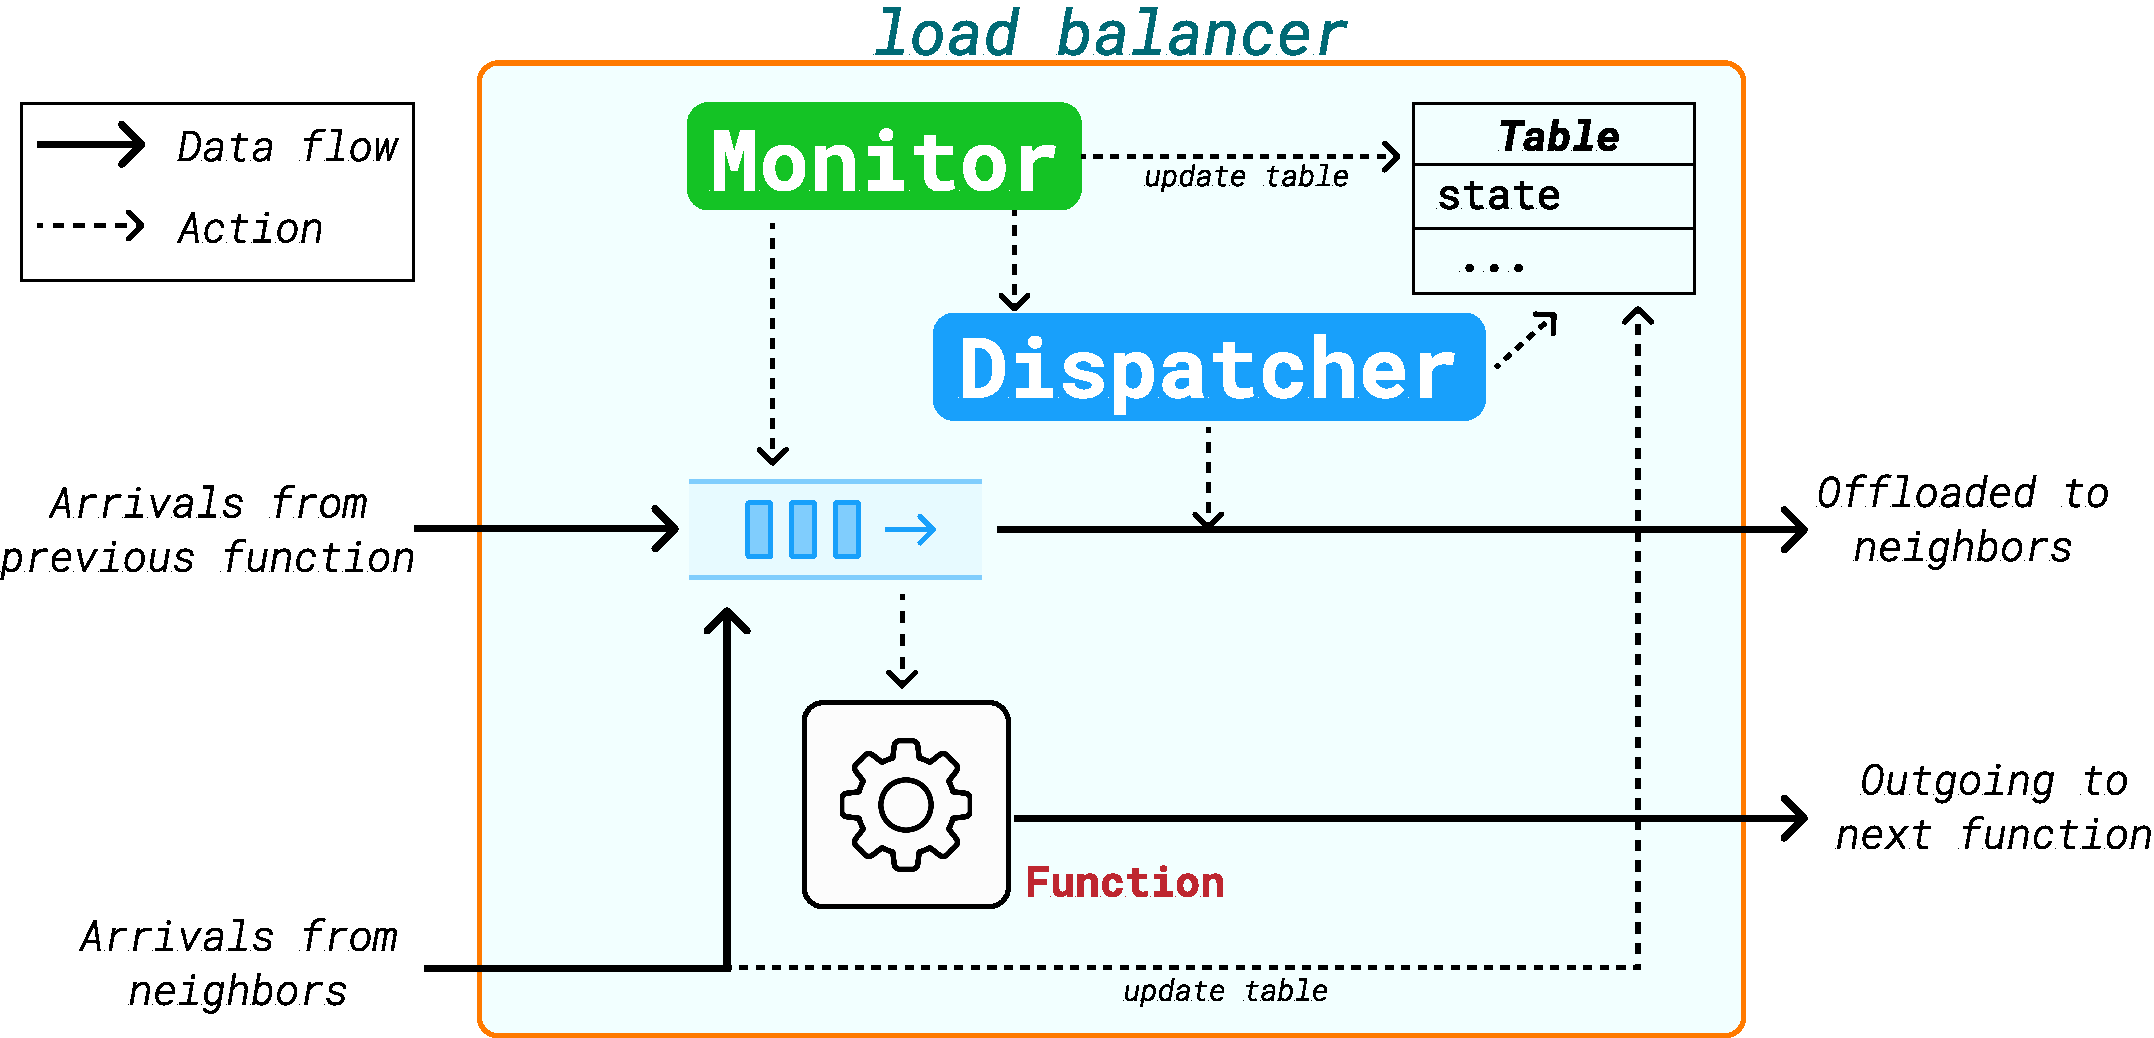
\includegraphics[width=\linewidth]{chapters/videojam/images/videojam_architecture.pdf}
    \caption{VideoJam's load balancer.}
    \label{fig:load_balancer}
\end{figure}

The core VideoJam's architecture leans on a set of load balancers, one associated with each and every replica the processing functions deployed among the set of available edge servers, as shown in~\Cref{fig:architecture}. In VideoJam, each load balancer (shown in~\Cref{fig:load_balancer}) communicates with the rest of load balancers installed on the functions of the same type (\eg, background subtractor, object recognition,~\etc), also called \textit{neighbors}. The load balancer wraps a function replica and mainly consists of two components: the \textit{Monitor} and the \textit{Dispatcher}. Through these two modules the load balancer takes decisions about incoming frames from the previous functions in the pipeline and from the neighbors to compute the (i) the output to the next function in the pipeline, and (ii) a load balancing policy, \ie, the amount of frames to be offloaded towards its neighbor. Such policy is calculated on the basis of a state table containing the information on the states of each neighbor, presented in rows. This information includes the estimates of load for the neighbors derived from predictions generated by a forecasting model. 

\subsection{Message Exchange}
In~VideoJam's system of load balancers, each component computes its state and load balancing policy based on local information, \ie, the incoming load from the previous function in the pipeline, and information collected from the neighbors acquired through a set of message interactions listed below. These mechanisms are designed to ensure that the load balancers converge to a common policy and compensate for potential errors in load forecasting.

\paragraph{Information Request.} Load balancers submit a request for neighbor state information when their local data is missing or obsolete. In this case, a load balancer sends, together with its table, an information request to its neighbor, asking for information about its status. Based on the response (described below), the receiver then updates its table according to the table received, substituting the rows containing obsolete information. 

\paragraph{State Update.} A state update is always sent by a load balancer in one of two scenarios: (i) at bootstrap to announce its presence to neighbors; (ii) after receiving an information request from one of its neighbors. State responses contain a summarization of the local system state, including current and forecasted loads, as well as expected incoming loads from neighbors. State updates are also sent when a prediction error is detected after receiving an offloaded workload from one of the neighbors. Such an error quantifies the difference between the expected load (according to the predictions) and the actual load received from the neighbor. 

\paragraph{Congestion Risk Signal.} A congestion risk signal is sent by a load balancer to one of its neighbors only when it detects, after updating its table and according to the last computed policy, that a given neighbor is transmitting offloaded traffic to itself, while this was not expected given previous exchanges, \ie, when the neighbor is not present in the list of neighbors from which it should receive offloaded video data.

\paragraph{Data Offloading.} Beyond the actual offloaded workload, the data transferred from a load balancer to one of its neighbors may also contain the sender's table. It is worth noting that a load balancer cannot receive workloads from the neighborhood while it is offloading to another neighbor. Hence, the receiver first checks whether it is offloading to one or more neighbors according to its computed policy. In this case, it recomputes the load balancing policy and checks whether, according to the new policy, it is supposed to receive some data. If not, it sends a congestion risk signal back to the sender. Otherwise, it receives the workload, computes the prediction error and sends a status update if the error is above a certain threshold. 

\subsection{System state computation}\label{sec:monitor}

In VideoJam, the system state is computed periodically and represents the current state of the load balancer based on the incoming load from the previous function in the pipeline, the processing rate, the queue size, and the offload rate to its neighbors. Here we formally describe the computation of the system state.

\paragraph{Operational Time Windows.} Each load balancer associated to function $c$, operates over a time windows $W^k_j$, which consists of $k \in \mathbb{N}^+$ consecutive time-slots and is defined as

\begin{equation*}
    W_{j} = W^k_{j} = \{w_i\}^k_{i=1},
\end{equation*}

where $w_i$ is the $i^{th}$ time-slot of the time window. All the time-slots within the time window have the same duration of $\Delta$ seconds. The next time window is denoted as $W_{j+1}$.

Each load balancer $S_{c,n}$ is characterized by its state, and keeps track of the states of all its neighbors (identified by $\mathcal{S}^*_{c}$) in a table. We further indicate with $S_{c}$ the set of all load balancers associated to function $c$ deployed among the edge nodes. 

\paragraph{State.} At each time window $W^k_{j} = \{w_i\}^k_{i=1}$, the state of load balancer $S_{c,n}$ is defined by (i) its processing rate $\mu_{c,n}$, (ii) the historical incoming load $\{\lambda^{c,n}_{w_i}\}_{w_i \in W^h_j}$ of $h \ge k$ previous time-slots, (iii) its current queue size $\varphi^{c,n}_{W_j}$, and (iv) the offload $\delta^c_n$, \ie, the total workload offloaded towards its neighbors. The table of each load balancer contains an estimation of all its neighbors' states. Such an estimation is based on the last information the load balancer has received from the neighborhood and it is updated every $r$ time windows. When this time expired, \ie, $r=0$, the load balancer sends an information request to the neighborhood. As shown in~\Cref{fig:load_balancer}, the interaction of the two main components, \ie, the Monitor and the Dispatcher, of each load balancer, determines the final offloading policy. We describe in detail how the dispatcher calculates the offloading policy in the next section.

The Monitor is in charge of monitoring the state and performance of the load balancer over time. More precisely, it supervises the incoming load from the prior function in the pipeline, and the processing rate. At each time-slot $w_i$ of a given time window, the monitor measures the amount of workload $\lambda^{c,n}_{w_i}$ coming from the previous function in the pipeline. At the end of each time window, the monitor updates the historical incoming load of the state of the load balancer by shifting its $h-k$ values to the left and replacing the last $k$ values with the load received in the window $W_{j}$. After such an update, the monitor triggers the Dispatcher for the computation of the load balancing policy.

\subsection{Load Balancer Algorithm}\label{subsec:dispatcher}
Here we describe in details the algorithm executed by each load balancer to compute its local offloading policy. The Dispatcher is in charge of computing the load balancing policy of VideoJam through the computation of the queue size and the prediction of future incoming workload for the load balancer. For a given function $c$, the policy is determined in such a way that the load is fairly distributed among all the load balancers in $\mathcal{S}_c$. In this manner, the load is processed at approximately the same time, as shown in~\cite{shah2007design}. Regarding the prediction of future incoming workload, given the limited capabilities of computational resources at the edge, state-of-the-art methods, such as Long Short-Term Memory (LSTM)~\cite{greff2016lstm}, result to be computationally intensive and, hence, prohibitive for the described scenario~\cite{lalapura2021recurrent}. Furthermore, when it comes to video analytics, learning the specific distribution of the load results to be a non-trivial task due to concept-drift problems~\cite{bhardwaj2022ekya},
%there is no specific distribution of load that can be learned,
especially when dealing with mobile cameras. For these reasons, the dispatcher relies on lightweight ML models to predict the incoming workload. In particular, we have developed a lightweight convolution-based neural network model based on a few convolution layers for predictions~\cite{KerasTCN}. This model presents fast inference time and high accuracy metrics. The complete pseudocode of the dispatcher is described in~\Cref{algo:dispatcher}.


\paragraph{Determine the Queue Size.} Within a given time window $W_{j}$, each load balancer determines the queue size $\varphi^{c,n}_{W_{j+1}}$, which is the load at the beginning of the next window $W_{j+1}$, by counting the amount of load currently waiting for processing (line 2 of~\Cref{algo:dispatcher}). The queue size of each neighbor $S_{c,m} \in \mathcal{S}_c^*$ is estimated
%For all $m$ in $\mathcal{S}^*_c$, the queue size is estimated 
by adding (i) the difference between the incoming load and the processing rate, and (ii) the total amount of workload exchanged with the neighborhood, to the previous expected load (lines 3--7 of~\Cref{algo:dispatcher}). More formally,
\begin{equation}
    \begin{split}
        \tilde{\varphi}^{c,m}_{W_{j+1}} = \tilde{\varphi}^{c,m}_{W_{j}} + \sum_{w_i \in W_{j}}(\lambda^{c,m}_{w_i} - \mu_{c,m}) + \delta^c_{m}, %\quad
        %\forall m \neq n, m \in \mathcal{N}, 
        %\forall w_i \in W_{k,j}}
    \end{split}
    \label{eqn:queue_size_estimation}
\end{equation}
where, $\delta^c_{m} = \sum_{p \in \mathcal{N}} \delta^c_{m \mid p}$, $\delta^c_{m \mid p}$ is the offload between $S_{c,m}$ and $S_{c,p}$, where $\delta^c_{m \mid p} < 0$ if data is offloaded from $S_{c,m}$ to $S_{c,p}$, and $\delta^c_{m \mid p} > 0$ if $S_{c,p}$ is sending data to $S_{c,m}$.

\paragraph{Predict Future Incoming Workload.} The load balancer forecasts its load and the incoming load of its neighbors for the next time window. For such predictions we rely on a convolution-based neural network model used to predict short-term workload~\cite{kombi2017preventive} (more details on the model are available in~\Cref{sec:implementation}). The input of the predictive model is the historical incoming load $W_h$ (\ie, $\{\lambda^{c,n}_{w_i}\}$ consisting of $h \ge k$ previous time-slots) for all load balancers. While the output is the incoming load for the next window $W_{j+1}$. So when the predicted workload deviates from the actual workload during the monitoring phase, the Monitor can detect it and react to make adjustments at any time.

\paragraph{Offloading Policy Computation.} 
Within a given time window $W_{j}$, each load balancer $S_{c,n}$ determines the offloading policy, \ie, $\delta_{n|m}^c$ for each $S_{c,m} \in \mathcal{S}_{c}$ for the next time-window $W_{j+1}$. Such a policy is computed through the following steps: 

(i)~First, the estimation of the global load, $\tilde{\phi}^{c,n}$, is computed according to 
\begin{equation}
    \tilde{\phi}_{c,n} = \tilde{\varphi}^{c,n}_{W_{j+1}} + \sum_{w_i \in W_{j+1}} \lambda^{c,n}_{w_i},
    \label{eqn:global_load_estimation}
\end{equation}
\ie, the estimated queue size at the beginning of the next time window plus the expected incoming load.  The queue size estimate is performed for all its neighbors in $\mathcal{S}_{c}^*$, whereas it can simply be obtained from the load balancer queue.

(ii)~Then, based on the estimation of the global load, each load balancer $S_{c,n}$ estimates the actual load that every load balancer in $\mathcal{S}_{c}$ should handle:
\begin{equation}
    \bar{\phi}_{c,n} = \frac{\sum_{n \in \mathcal{N}}\tilde{\phi}_{c,n} * \mu_{c,n}}{\sum_{n \in \mathcal{N}} \mu_{c,n}}, %\forall n \in \mathcal{N}
    \label{eqn:balanced_load_estimation}
\end{equation}
where $\tilde{\phi}_{c,n}$ is the global load that should be processed by $S_{c,n}$ with a process rate of $\mu_{c,n}$, and $\sum_{n \in \mathcal{N}} \mu_{c,n}$ is the total processing capacity of all the load balancers associated to function $c$.

(iii)~The load balancer computes the \textit{unbalanced} load for all the load balancers associated to function $c$ (line 12 in~\Cref{algo:dispatcher}) as 
\begin{equation}
    \theta_{c,n} = \bar{\phi}_{c} - \tilde{\phi}_{c,n}. %\forall n \in \mathcal{N}
    \label{eqn:unbalanced_load_estimation}
\end{equation}
Positive values for $\theta_{c,n}$ indicate that the function associated to the load balancer will be underutilized. In this case, it should receive workload from neighbors $S_{c,m}$ with negative values of $\theta_{c,m}$. Negative values for $\theta_{c,n}$, on the other hand, point out that the function will be overloaded requiring to offload some workload to the neighbors.

(iv)~Finally, the amount of workload to be offloaded towards each neighbor $S_{c,m}$, \ie, the offloading policy $\delta^c_{n \mid m}$, is finally computed based on $\theta_{c,n}$ as described from line 14 to 27 of~\Cref{algo:dispatcher}. Until all the $\theta$'s are set to $0$, the dispatcher takes the most loaded $S_{c,n}$ to balance to the least leaded $S_{c,m}$ in $S_c$. The load is transferred from $S_{c,n}$ to $S_{c,m}$ if there is enough room for the load, and the unbalanced load of $S_{c,n}$ is set to $0$. Otherwise, $S_{c,n}$ transfers to $S_{c,m}$ the maximum load that can be received $\theta_{c,m}$ and the unbalanced load of the receiver is set to $0$.

\begin{algorithm}[t]
\caption{Dispatcher algorithm procedure}
\label{algo:dispatcher}
\SetAlgoLined
\SetKwProg{Fn}{Function}{}{end} % Function name(args) [...] end
\Fn{dispatcher($\varphi$, $\lambda$, $\mu$, $\delta$, $\mathcal{S}_{c}$)}
{
\begin{small}
\tcc{1. Determine the queue size}
$\varphi^{c,n}_{W_{j+1}} = getQsize()$

\tcc{1. Estimation load for neighbors, \ie, $\mathcal{S}_c^*$}
\For{ $S_{c,m} \in \mathcal{S}_{c}^*$ } 
{
    $\tilde{\varphi}^{c,m}_{W_{j+1}} = \tilde{\varphi}^{c,m}_{W_{j}} + \sum_{w_i \in W_{j}}(\lambda^{c,m}_{w_i} - \mu_{c,m}) + \delta^c_{m}$\;
}
\For{ $S_{c,n} \in \mathcal{S}_{c}$ }
{
    \tcc{2. Forecast the future incoming load, \ie, $\lambda^{c,n}_{w_i}, w_i \in W_{j+1}$}
    $\lambda^{c,n}_{w_i} = model(\{\lambda^{c,n}_{w_i}\}_{w_i \in W^h})$\;

    \tcc{Estimation of global load}
    $\tilde{\phi}_{c,n} = \tilde{\varphi}^{c,n}_{W_{j+1}} + \sum_{w_i \in W_{j+1}} \lambda^{c,n}_{w_i}$\;
}


\tcc{Compute the unbalanced load}
\For{ $S_{c,n} \in \mathcal{S}_{c}$ }
{
    \tcc{balanced load $\bar{\phi}_{c,n}$}
    $\bar{\phi}_{c,n} = \frac{\sum_{n \in \mathcal{N}}\tilde{\phi}_{c,n} * \mu_{c,n}}{\sum_{n \in \mathcal{N}} \mu_{c,n}}$\;
    \tcc{unbalanced load}
    $\theta_{c,n} = \bar{\phi}_{c} - \tilde{\phi}_{c,n}$
}

\tcc{3. Compute the offloading policy}
\While{ $\text{any($\theta_{c,n} < 0$) and any($\theta_{c,n} > 0$)}$ }
{
    \tcc{the most overloaded}
    $n = argmin(\theta_{c})$\;
    \tcc{the less overloaded}
    $m = argmax(\theta_{c})$\;
    $q = \lvert \theta_{c,n} \lvert$\;
    \uIf{ $q < \theta_{c,m}$ }{
        \tcc{load from $S_{c,n}$ to $S_{c,m}$}
        $\delta^c_{n \mid m} = q$\;
        $\theta_{c,n} = 0$\;
        $\theta_{c,m} = \theta_{c,m} - q$\;
    }
    \Else{
        $\delta^c_{n \mid m} = \theta_{c,m}$\;
        $\theta_{c,n} = \theta_{c,n} + \theta_{c,m}$\;
        $\theta_{c,m} = 0$\;
    }
}
\end{small}
    }
\end{algorithm}


\section{Implementation and Deployment Configuration}
\label{sec:implementation}

In this section we present the details on how we implement~VideoJam, \ie, the set of parameters of the architecture and the video analytics components. Further, we present our evaluation setup, including the evaluation metrics, the datasets we have select for evaluating the system, and the baselines we compare VideoJam with.

\subsection{Prototype Implementation}

We implement VideoJam with about 400 lines of Python 3 code, using the asyncio~\cite{asyncio} library to handle I/O operations of incoming frames and objects to process, and OpenCV v4.5.3 with CUDA v11.2.2 support for various vision models. With its simple design,~VideoJam offers flexibility in incorporating any existing project, since only the communication component and the actual function (\eg, a Deep Neural Network model), are needed to be adapted to the existing one. The library is designed to easily support a variety of existing video analytics applications. We integrate the system in a docker image can be pulled from a public docker hub or built from the Dockerfile available in our public GitHub repository~\footnote{The VideoJam implementation code is freely available at \href{https://github.com/ENSL-NS/VideoJam.git}{https://github.com/ENSL-NS/VideoJam.git}}. To evaluate the design effectiveness, we implement the functions of a typical traffic control application: vehicles' number plate detection.


\paragraph{Video Analytics Components.} We implement the vehicles' number plate detection pipeline by integrating the following video analytics functions: video source and decoder, background subtractor and vehicle detection (for fixed camera sources), YOLO object detection (for mobile sources), and number/license plate recognition.

\begin{figure}
	\centering
	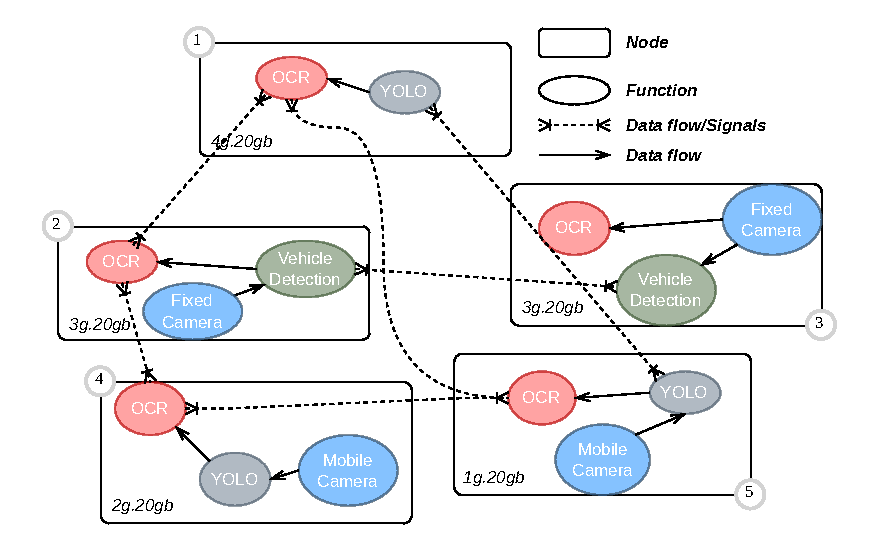
\includegraphics[width=\linewidth]{chapters/videojam/images/videojam_example_of_deployment.pdf}
	\caption{An example of heterogeneous deployment of VideoJam. Note that not all links between functions are represented to reduce image complexity.}
	\label{fig:example_deployment}
\end{figure}

The decoder represents the entry point of the pipeline and takes as input an encoded stream (for the evaluation in this paper we use pre-recorded videos, yet the system supports live streams as well). The decoded video frames are then passed on to the next function for further processing.

For fixed cameras, frames are transmitted to the background subtractor. The background subtractor is a function that generates a foreground mask using a static camera. This mask is then used on the current image to subtract the static scene, \ie, the background, while each moving scene is detected and classified as an object of interest. Extracted objects are then passed to the vehicle detection function, which embeds a machine learning model trained to detect vehicles within an image~\cite{vehicle_detection}. Detected vehicles are passed along to the next function, while other objects are discarded.

For detecting vehicles in mobile sources, we integrate a YOLOv5 model~\cite{jocher2020yolov5}. YOLOv5 is the fifth version of the YOLO (You Only Look Once) object detection model. It performs detection and classification, and returns a box for each object in the image taken in input, along with their classes with a high degree of accuracy. This is computationally intensive and is generally used on GPUs to achieve fast and accurate results in real-time. There are many pre-trained check-points available, as well as input size pixel images. For our purposes, we use YOLOv5s with a high (640) and low (416) input pixels size. 

Finally, detected vehicles are passed to an object character recognition (OCR) function that used to detect license plates on cars. Numerous frameworks have been developed for this task. In our implementation we integrate Tesseract~\cite{ocr}, an open source OCR engine that combines traditional image processing techniques with modern machine learning methods to accurately recognize and convert text from images into a digital format.

We use these functions to create a heterogeneous application with two different pipelines. The first takes as input fixed video camera feeds passed along to the background subtractor, which forwards the data to the vehicle detector for classification before the final function, the license plate detection. The second pipeline takes data from a moving camera and processes them using YOLO, then passes the result to the license plate detection. This last function is shared by both pipelines for reuse and optimization. With such a deployment, a situation of workload imbalance can arise at any time, and forecasting becomes more challenging. The complete application used for deployment is presented in \Cref{fig:example_deployment}. All functions (except sources and background subtractor) of the same kind run load balancing and implement the~VideoJam monitor and dispatcher. We have avoided drawing all the lines between the pairs (as specified in the caption) to avoid increasing the complexity of the figure.

\paragraph{System configuration and model tuning.} We configure the VideoJam load-balancing system using the parameters summarized in~\Cref{tab:configuration}. Regarding the predictive model, we opt for an architecture that minimizes inference time while guaranteeing acceptable performance. We choose a neural network (NN) with a single dense layer of 512 units trained over 100 epochs. The model takes in input a window of size $h$ and can predict a window of size $k$ (see~\Cref{tab:configuration} for the values of these parameters). We also tried out different architectures, such as a convolutional neural networks (CNN), and LSTMs. However, such models result to be difficult to use since (i) CNN requires a significant amount of time for the inference, although it has high levels of accuracy; (ii) in our case, LSTM presents poor performance in terms of both accuracy and inference time given its specific use on time series (different from our case).

\begin{table}
	\centering
	\begin{tabular}{p{1.5cm}p{6.5cm}}
    \toprule
	\textbf{Parameter} & \textbf{Value and description}                                                          \\
	\midrule
	\textbf{$\Delta$}  & 1 second (the monitoring duration)                                                      \\
	\textbf{$k$}       & 10, represents a monitoring window of $10*\Delta=10$ seconds                            \\
	\textbf{$h$}       & 50, the history for short-term forecasting                                              \\
	\textit{model}     & short-term forecasting: DNN for Vehicle detection and Number plate OCR, none for YOLOv5 \\
	\bottomrule
	\end{tabular}
	\caption{VideoJam configuration~\label{tab:configuration}}
\end{table}

\subsection{Evaluation Setup}\label{sec:setup}

\paragraph{Baselines.} We evaluate VideoJam compared against three different baselines: (i)~a video analytics pipeline that does not implement any load balancing, (ii)~one that implements Weighted Round Robin (WRR), and (iii)~Distream~\cite{zeng2020distream}, a state-of-the-art solution. In WRR, neighbors determine their processing rates based on an initial estimation, share this information with their neighbors, and collectively assign weights based on their capacity to create a load-balancing policy. They then apply this policy to distribute incoming workload to their local queues or to neighbors, with offloaded work being placed directly in a neighbor's local queue. For Distream, we start with the version available at the project repository\footnote{https://github.com/AIoT-MLSys-Lab/Distream/tree/main}. We then transform the Golang code into Python for integration into our deployment framework. Finally, we also adapt the code to support batch processing, mentioned in the article but not implemented in the open source version. The final code is also available on our public GitHub. Note that Distream does not support heterogeneous pipelines, thus we solely integrate the pipeline with YOLO into its architecture.

\paragraph{Deployment Infrastructure.} We conduct experiments deploying multiple docker containers on a server machine equipped with Nvidia A100 GPUs (full specifications are shown in~\Cref{tab:grid5000}). For functions necessitating access to GPU resources, we leverage the MIG (Multi-Instance GPU) that Nvidia GPU offers to split the available GPUs into multiple instances. We emulate a heterogeneous edge infrastructure by splitting the GPU into six nodes with heterogeneous compute cores (\ie, \textit{4g.20gb}, $2\times$~\textit{3g.20gb}, \textit{2g.10gb} and $2\times$~\textit{1g.5gb})~\cite{nvidiamig}. Given the lack of enough CPU cores we leave all containers to concurrently use all available CPUs. While this reduces the realism in terms of CPU isolation, the implemented functions mostly rely on the GPU for heavier computations, thus not introducing unwanted bottlenecks to the setup. Finally, regarding network connectivity between containers, we emulate a realistic network configuration to the extent possible. For this reason, we not only limited the links between nodes to 1gbps, but also configured these links to have realistic latencies and bursts. For information, we used the following \textit{tc} command: \textit{rate 1gbit burst 16kbit latency 10ms}.

\begin{table}
	\centering
	\begin{tabular}{p{1cm}p{7cm}}
    \toprule
	\textbf{Model}  & Dell PowerEdge R7525                           			\\
	\textbf{CPU}    & AMD EPYC 7452 (Zen 2), 2 CPUs/node, 32 cores/CPU  	\\
	\textbf{Memory} & 128 GB																							\\
	\textbf{GPU}    & 2 x Nvidia A100-PCIE-40GB, Compute capability: 8.0	\\
	\bottomrule
	\end{tabular}
	\caption{Server configuration used for experiments.}
	\label{tab:grid5000}
\end{table}

\paragraph{Evaluation metrics.} We evaluate the performance of VideoJam and the other baselines using three metrics: (i) the response time, (ii) the loss rate, and (iii) the total bandwidth utilization. The response time for a frame refers to the time elapsed from its introduction into the system (\ie, from the source)
to its complete processing by the last function in the pipeline. It can also be measured at the level of a specific pipeline function. For example, the response time for a frame measured at the vehicle detection level corresponds to the time elapsed between its entry into the pipeline and its exit from this function. A low response time is an indicator of the system's ability to quickly extract the
information generated by the application. The percentage of losses corresponds to the number of objects lost over the total number of objects to be processed.
In general, each function has a queue with a maximum number of items that can be held in it. When the incoming load exceeds a function's capacity, it begins to accumulate load in its queue. When the queue is full, any new incoming objects arrive they are dropped. Since we do not focus on function selection, losses
become the main indicator of accuracy reduction. Finally, total bandwidth utilization corresponds to the total amount of data transmitted during load balancing between functions. This is an important measure, as it enables us to measure the impact of the different approaches used on network resources.

\paragraph{Datasets.}
We use public real-world videos from YouTube for both fixed and mobile cameras. We selected a custom dataset of videos from YouTube for three reasons: (i) Existing mobile video datasets did not meet our requirements. For example, the BDD100k dataset~\footnote{http://bdd-data.berkeley.edu/}, widely used for analytics tasks, contains a good collection of traffic datasets from an on-board camera on cars in different weather conditions. However, the dataset contains only short sequences of videos lasting less than a minute or using under-sampled images. (ii) Using YouTube videos is a common standard in the state-of-the-art~\cite{zeng2020distream,zhang2022batch,lai2021top,wang2020surveiledge,elgamal2020sieve}. (iii) The selected dataset meets the diversity of requirements for the evaluation in this paper. The videos we selected include 11 videos from dashboard cameras mounted on cars traveling through various cities (\eg, Los Angeles~\footnote{https://www.youtube.com/watch?v=Cw0d-nqSNE8}), and nine fixed cameras mounted on street corners in the same cities~\footnote{https://www.youtube.com/watch?v=wqctLW0Hb\_0}. These recordings come in a variety of conditions, including normal to heavy traffic, as well as empty and crowded locations. As a result, the number of vehicles (\eg, cars, trucks) in the frames of these videos are variables, with minimum, maximum, mean, and median respectively of 0, 15, 3, and 3 per frame. Further, these videos are longer than the ones described in the previous dataset, and they span between 5 and 80 minutes (see~\Cref{tab:dataset}).

\begin{table}
	\centering
	\begin{tabular}{p{1.9cm}p{1.9cm}p{1.7cm}p{1.7cm}}
	\toprule
	\textbf{Type of camera} & \textbf{Duration (min)} & \textbf{Resolution} & \textbf{Total videos} \\
	\midrule
	Mobile        & 11-80                                                                                                     & 720p                & 9                      \\
	Fixed         & 5-60                                                                                                      & 720p                & 11                     \\
	\bottomrule
	\addlinespace        
	\end{tabular}
	\caption{Video cameras used for experiments.}
	\label{tab:dataset}
\end{table}

% Experimental Evaluation
\section{Evaluation}\label{sec:evaluation}

We evaluate VideoJam in different scenarios and against the three baselines previously described. First, we compare it against Distream~\cite{zeng2020distream} to demonstrate the benefits of localized load balancing at function level, rather than a centralized approach for global load balancing. Next, we evaluate the system under different levels of loads to measure the performance of VideoJam as the workload increases. In addition, we test VideoJam's ability to adapt to system configuration changes or failures, by subjecting it to critical situations such as the failure of a function or the failure of a node. Finally, we test the system's ability to deal with mobile cameras leaving and joining the architecture, demonstrating VideoJam's ability to adapt to forecasting errors caused by sudden changes of video content.

\subsection{Comparison with Distream}
%In this experiment we compare VideoJam against a state-of-the-art video analytics architecture, Distream~\cite{zeng2020distream}. 
Distream's load balancing architecture is based on two main key concepts: the cross-camera workload and the partition point. The cross-camera workload determines the workload balance among cameras (also called ``Ends'') only. The partition point defines which functions of each pipeline are processed by Ends, while other functions are then executed on the server (called ``Edge''). The choice of offload proportion is handled in one of two different ways by the Ends: either a \textit{full-stochastic} (FS) or \textit{semi-stochastic} (SS) partitioning. In full-stochastic partitioning, the Ends generate a random partitioning proportion based on a Bernoulli random variable with probability set proportionally to the compute power of the Edge and End nodes. At every step of the pipeline, Ends draw a value from this variable and determine whether to process the function locally or offload it to the Edge. In semi-stochastic, the random value is drawn only at the partition point. In this case, the partition point is calculated as the point in the pipeline that evenly splits it proportionally to the compute power of the two components. 

\paragraph{VideoJam outperforms baselines in heterogeneous deployments.} We compare VideoJam and other baselines in dealing with mixed traffic of mobile and fixed video cameras. To carry out this experiment, we deploy Distream using five GPU-equipped nodes (as described in~\Cref{sec:implementation}). We deploy one instance of YOLO and one instance of OCR on each node, as required by Distream. We use the same five nodes for VideoJam, but we partition nodes hosting the pipeline for fixed and mobile cameras. In particular, we deploy two vehicle detection instances, three YOLOs, and five OCRs. We also deploy two other baselines, WRR and a VideoJam version that solely employs YOLOs for detection, and using the same configuration as VideoJam. Finally, we use four video sources, two mobile cameras and two fixed ones, draw randomly from the dataset presented in~\Cref{sec:implementation} and set to 20 frames per second. 

~\Cref{fig:distream_vs_videojam_heterogeneous} shows that VideoJam outperforms all other solutions, both in terms of response time, with 2.91$\times$ and 1.77$\times$ less response time compared to Distream's solutions, and reduces objects loss by 19\% and 4\%, respectively. This highlights the advantages of using a localized load balancing technique like VideoJam, and the limitation of approaches like Distream or a simplistic WRR. Further, the figure highlights that the use of mixed pipelines for different sources of traffic improves response time.  Indeed, the use of dedicated pipelines for fixed and mobile cameras, \ie, background substractor vs YOLO as explained~\Cref{sec:background_motivation}, improves classification performance incurring less load depending on the number of objects in each frame. Consequently, if the amount of objects in the video scene is low, no action, \ie, inference, will be taken, whereas detection techniques such as YOLO will take action even if no objects are present in the frames. This is supported by the performance improvement observed when comparing the two approaches on VideoJam (\ie, the one using vehicle detection over the one using only YOLOs). Furthermore, the results show that VideoJam has a response time 1.11$\times$
lower than VideoJam with YOLO only.

\begin{figure}
	\begin{minipage}[t]{.52\linewidth}
		\centering
		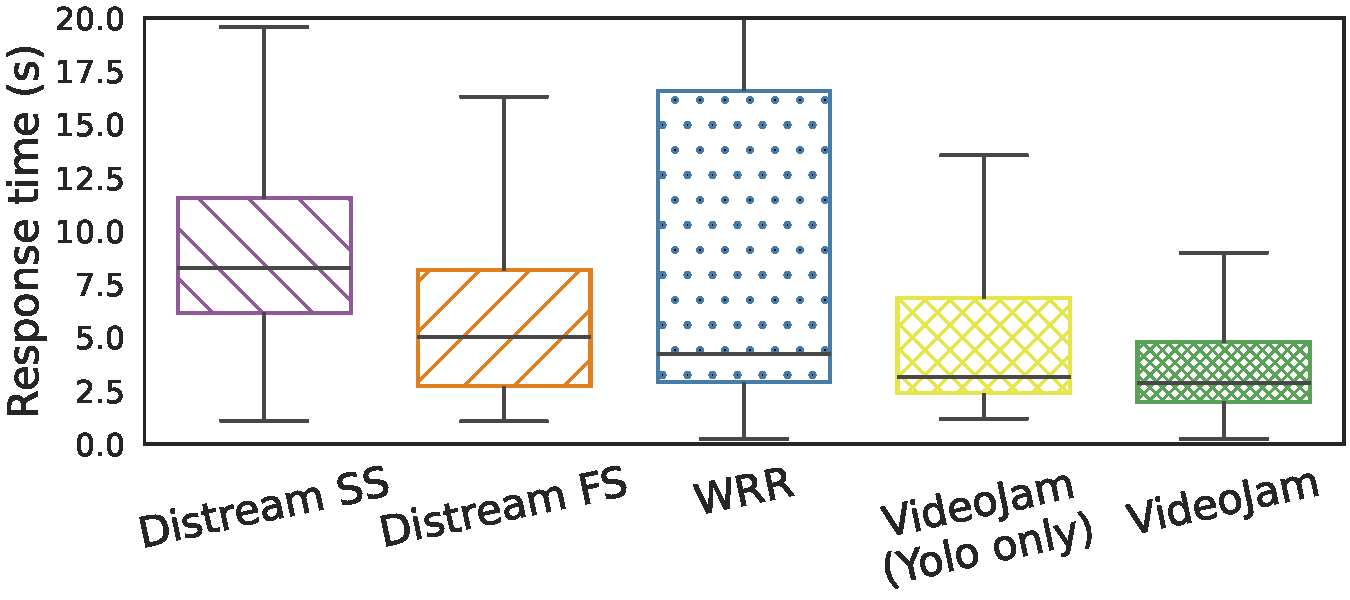
\includegraphics[width=\linewidth]{chapters/videojam/images/distream_vs_videojam/heterogeneous/response_time.pdf}
		\subcaption{Response time.}
	\end{minipage}
	\hfill
	\begin{minipage}[t]{.46\linewidth}
		\centering
		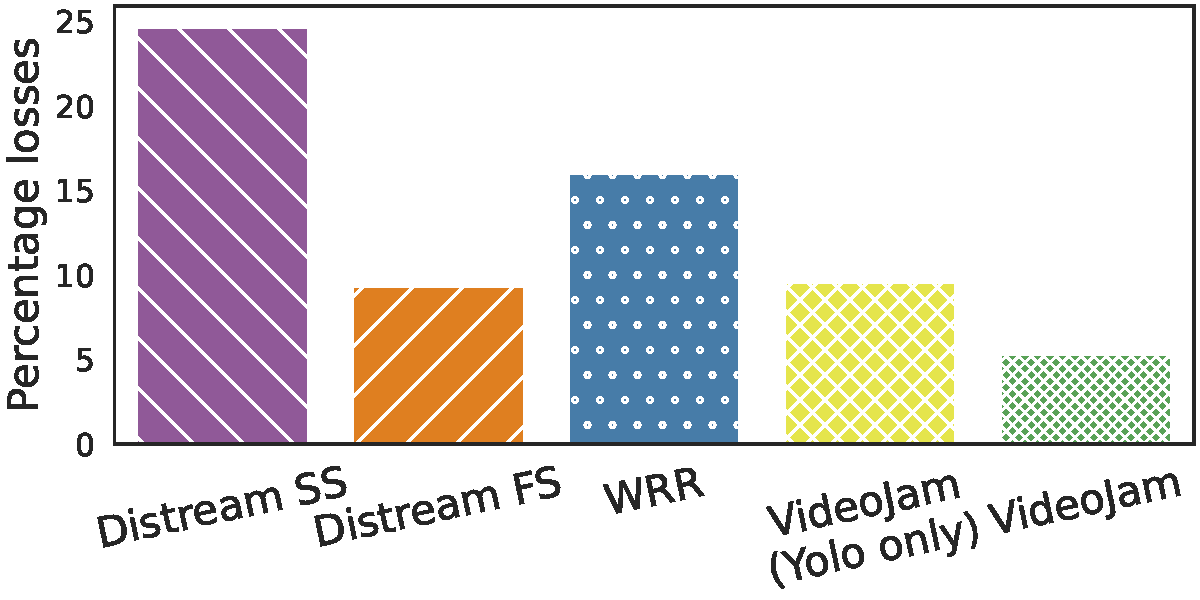
\includegraphics[width=\linewidth]{chapters/videojam/images/distream_vs_videojam/heterogeneous/percentage_losses.pdf}
		\subcaption{Percentage losses.}
	\end{minipage}
	\caption{Evaluation on a heterogeneous architecture shows a response time up to 2.91$\times$ lower than comparative approaches, and with fewer losses.}
	\label{fig:distream_vs_videojam_heterogeneous}
	\vspace{-3mm}
\end{figure}

\paragraph{VideoJam outperforms Distream in mobile only scenarios.} In the previous experiment we have shown that VideoJam outperforms baselines when processing mixed types of video traffic. We now explore whether our solution can still outperform Distream when solely processing video traffic generated by mobile cameras. We do so to evaluate VideoJam's load balancing technique, understanding whether the advantages presented previously are to be solely attributed to the use of different pipelines for different types of traffic or to the load balancing as well. In this experiment, we use the same experimental setup as in the previous experiment, the only difference being that we use YOLOs throughout the deployment for all baselines, and we use four mobile cameras.

~\Cref{fig:distream_vs_videojam} shows the performance of WRR, Distream, and VideoJam. We can observe that the semi-stochastic version of Distream incurs the worst performance in terms of both response time and loss: about 2.02$\times$ and 3.68$\times$, respectively, compared to VideoJam. Indeed, given the design of Distream, it is difficult to define the load balancing policy when considering the pipeline as a whole. In fact, two different functions (\eg, YOLO and OCR) on different nodes may become overloaded as traffic loads vary in time. This makes it very difficult to define an optimal load balancing policy for load distribution. Furthermore, in our observation, the considerable loss observed is due to the fact that a large portion of the video traffic remains continuously blocked in the Edge, which is unable to empty it quickly enough.

\begin{figure}
	\begin{minipage}[t]{.52\linewidth}
		\centering
		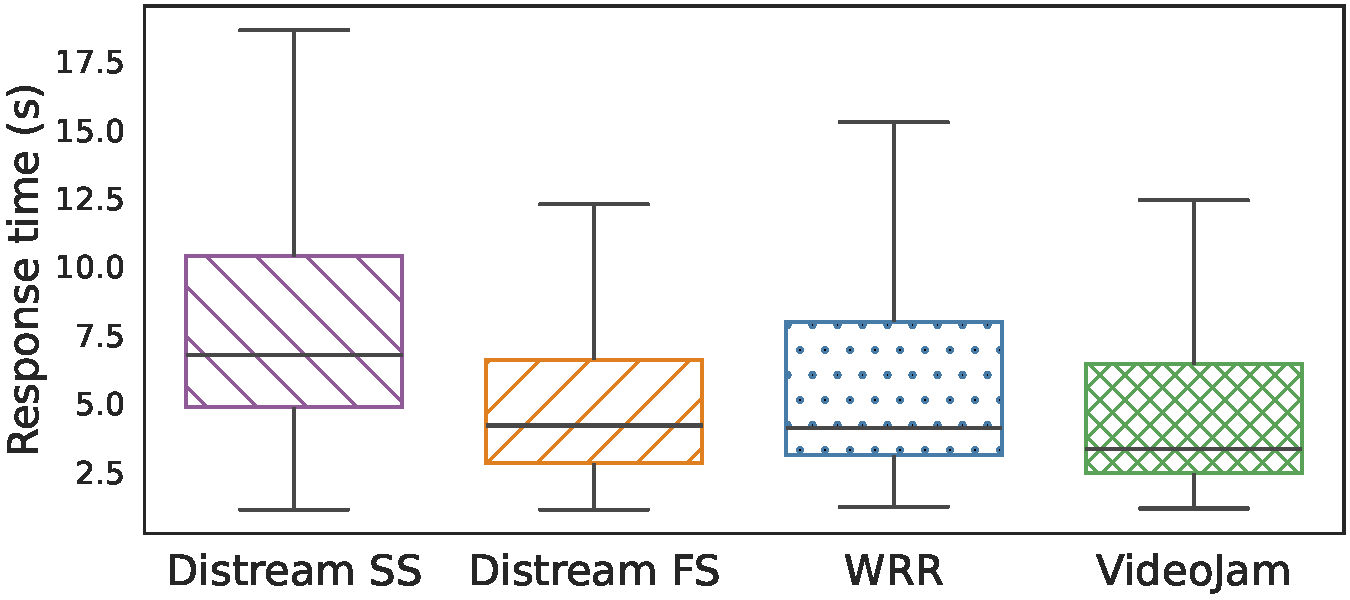
\includegraphics[width=\linewidth]{chapters/videojam/images/distream_vs_videojam/response_time.pdf}
		\subcaption{Response time.}
	\end{minipage}
	\hfill
	\begin{minipage}[t]{.46\linewidth}
		\centering
		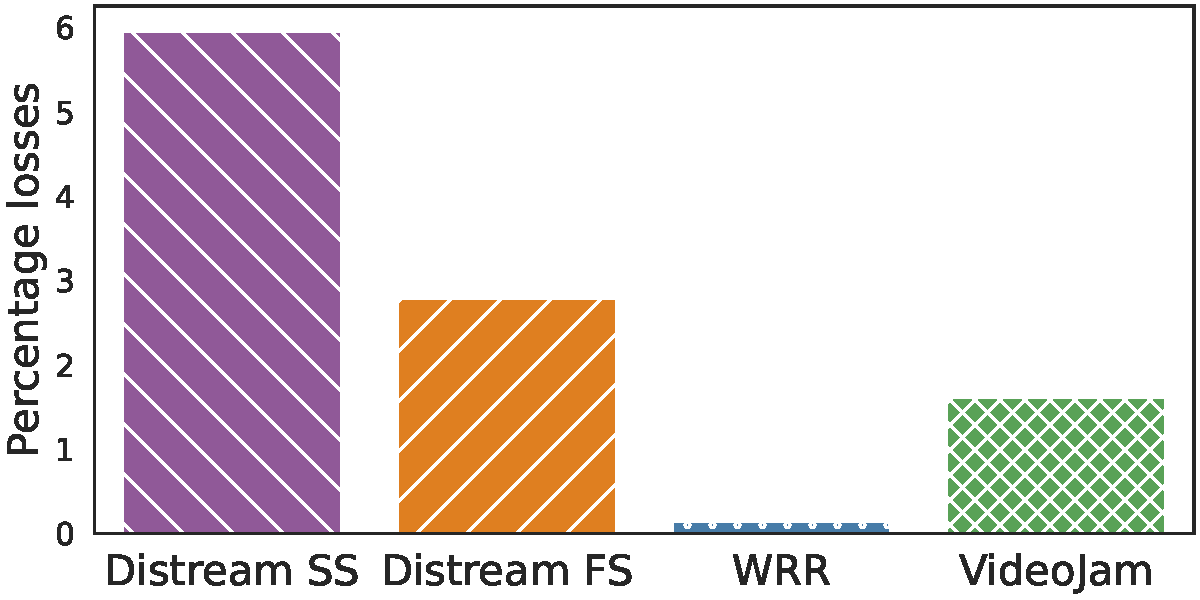
\includegraphics[width=\linewidth]{chapters/videojam/images/distream_vs_videojam/percentage_losses.pdf}
		\subcaption{Percentage losses.}
	\end{minipage}  
	\vspace{-1mm}
	\caption{Evaluation on mobile cameras shows that VideoJam's response time is 1.25$\times$ shorter than Distream's.}
	\vspace{-3mm}
	\label{fig:distream_vs_videojam}
\end{figure}

Nevertheless, we observe similar response time results between the full-stochastic approach and~VideoJam. The reason for this lies behind the simple offload policy implemented in this approach: as the pipeline consists of only two functions, the partition is only necessary at either YOLO or OCR, often leaving the Edge in charge of the full processing. Yet, this simplicity can incur increased loss, when these nodes become overloaded (about 3\% loss). We also observe that WRR experiences a lower percentage of loss compared to VideoJam. This is due to WRR's simpler load-balancing policy, which in some cases can be beneficial to loss, when frames spend more time being transmitted between nodes, slowing down the volume of traffic reaching the OCRs. In fact, we observe that WRR tends to balance load more aggressively across all available instances, thus increasing network usage (more details on this later in this section). Consequently, these frames are not queued fast enough to fill the ORC queues, explaining the small loss for WRR. This also explains the WRR's lower performance in terms of response time (1.22$\times$ lower response time than WRR). Ultimately, this shows that in certain instances, there might be a tradeoff to explore between response time and information loss. We leave this exploration for future work.



\paragraph{VideoJam better handles node failures.} The aim of this experiment is to determine the impact of node failure on the performance of Distream, WRR, and VideoJam. To do this, we simulate two types of failure: the first is an End failure, the second an Edge failure.

~\Cref{fig:distream_vs_videojam_onfailure} summarizes the performance of each solution. We can observe a significant loss for Distream (about 15\% of the total traffic). The reason for this large loss is that after the Edge has failed, the last policy calculated by the Edge, \ie, the partitioning point, is still executed by the Ends and is not updated during the Edge's absence. So when the Edge comes back, the computation it is supposed to be dealing with since the last partition point update suddenly arrives, saturating the Edge in the process and causing several losses. Also, Distream's low response time is due to the fact that fewer frames are waiting in the queue to be processed after a large proportion of them have been lost.

Furthermore, we see the ability of VideoJam to be robust to failures and to react a recovery. Indeed, when a node failure occurs, VideoJam adapts the load balancing policy calculation to the available resources. When the failed node returns, the policy is recomputed and all the workload already accumulated is redistributed. This explains the low losses of around 2\% which are 6$\times$ lower than Distream's ones. WRR, on the other hand, does not present the same ability of robustness to failures, even though its policy is updated every time the system is stressed. And since its policy does not take into account the workload of the instances, the load previously accumulated during the downtime is not redistributed.

\begin{figure}
	\begin{minipage}[t]{.52\linewidth}
		\centering
		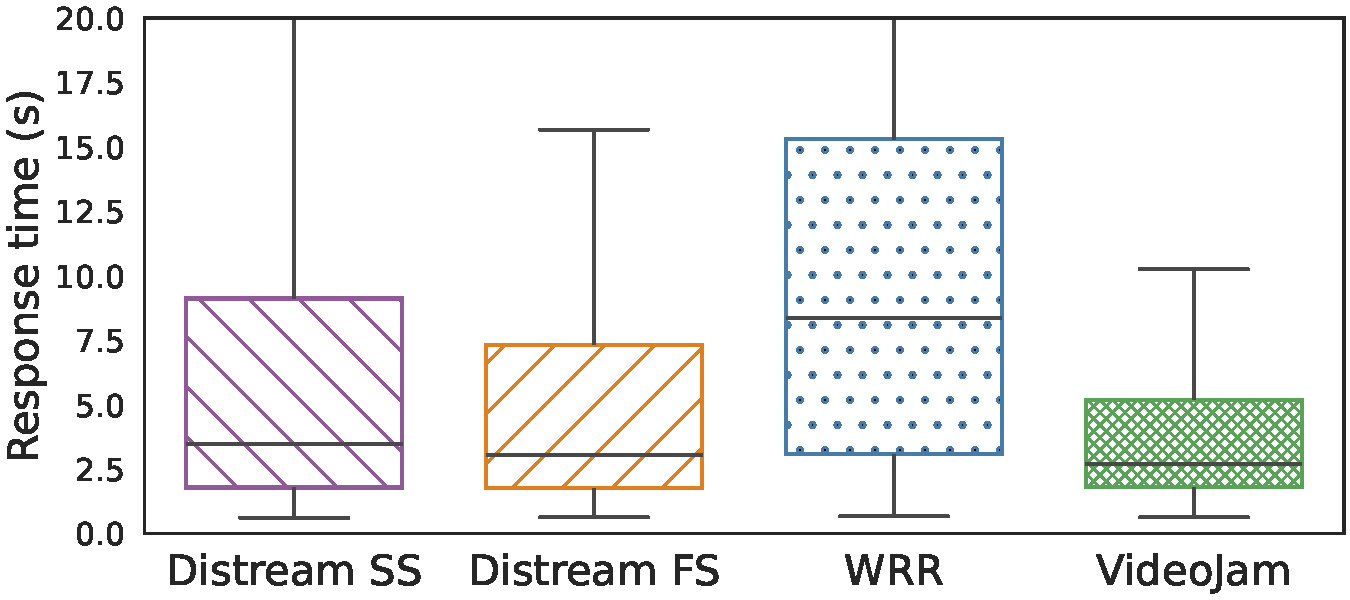
\includegraphics[width=\linewidth]{chapters/videojam/images/distream_vs_videojam/onfailure/response_time.pdf}
		\subcaption{Response time.}
	\end{minipage}
	\hfill
	\begin{minipage}[t]{.46\linewidth}
		\centering
		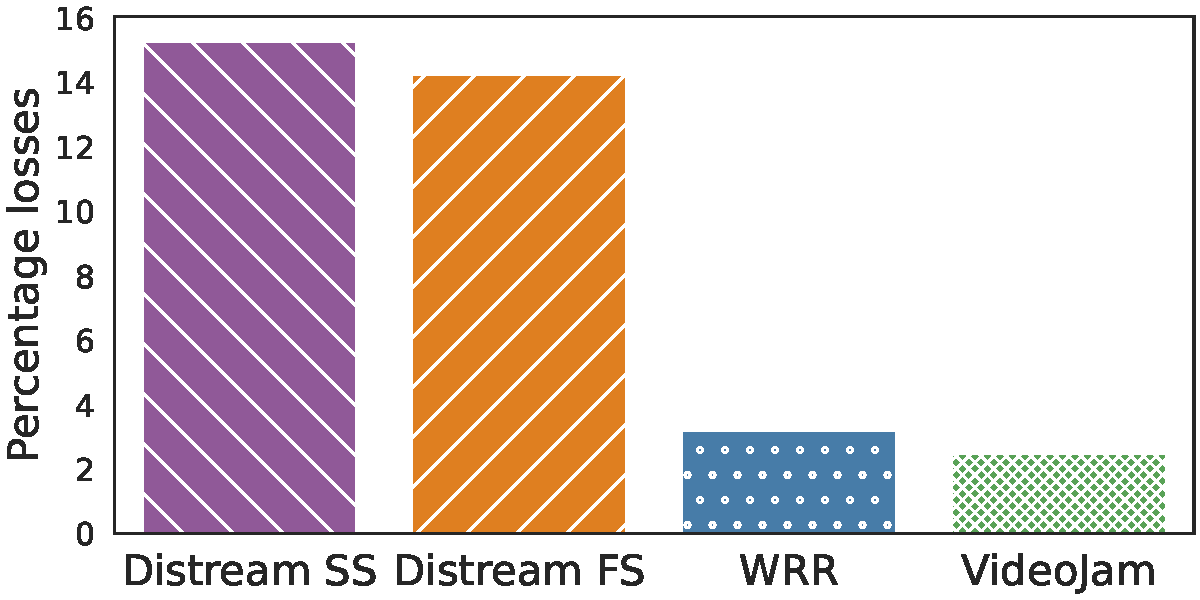
\includegraphics[width=\linewidth]{chapters/videojam/images/distream_vs_videojam/onfailure/percentage_losses.pdf}
		\subcaption{Percentage losses.}
	\end{minipage}
	\vspace{-1mm}
	\caption{Evaluation of Distream and VideoJam in the event of node failure, with the latter recording fewer losses while maintaining better response time.}
	\vspace{-3mm}
	\label{fig:distream_vs_videojam_onfailure}
\end{figure}



\subsection{Load Balancing Ablation Study}

In this section, we evaluate the effectiveness of VideoJam's load balancing algorithm with respect to two alternative baselines, no load balancing and WRR.

\begin{figure*}[htb]
	\centering
	\begin{minipage}[t]{.3\linewidth}
		\centering
		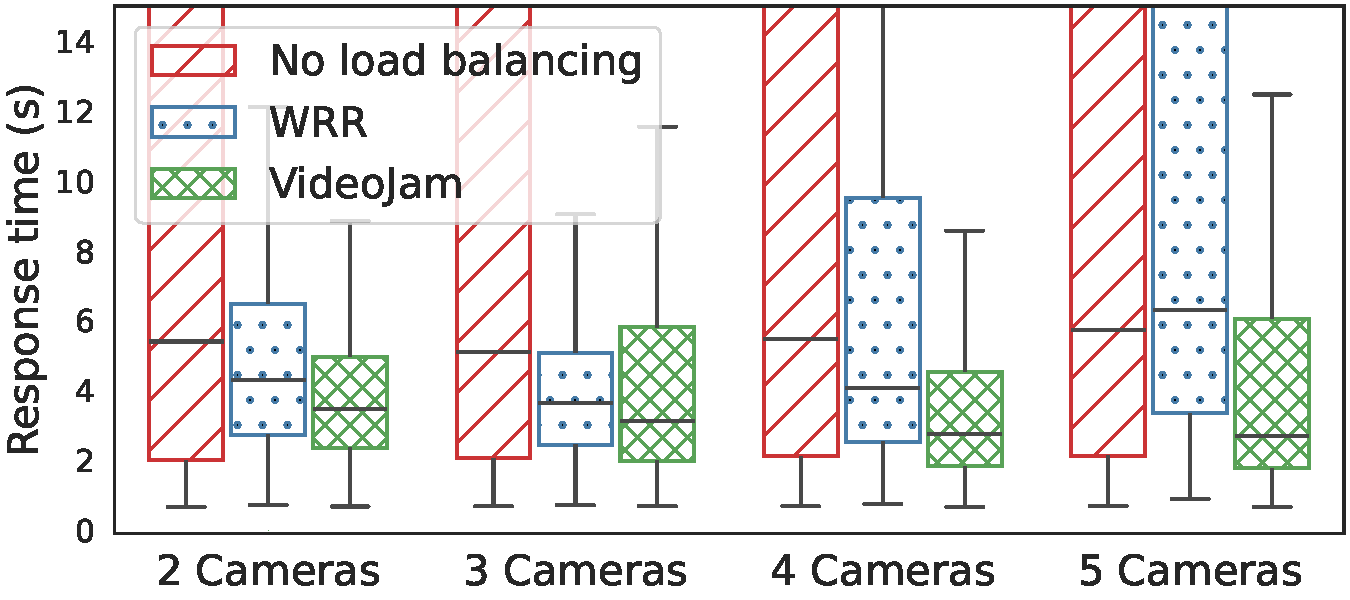
\includegraphics[width=\linewidth]{chapters/videojam/images/agains_weighted_roundrobin/response_time.pdf}
		\subcaption{Response time of the system.}
	\end{minipage}
	\hfill
	\begin{minipage}[t]{.3\linewidth}
		\centering
		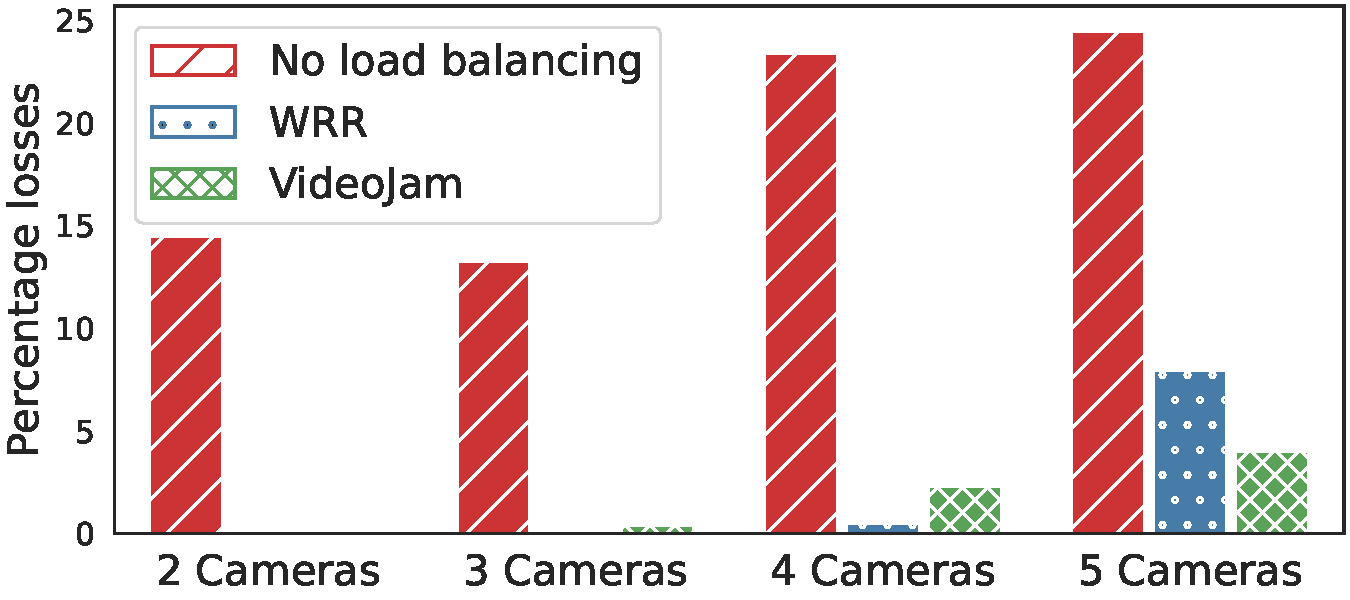
\includegraphics[width=\linewidth]{chapters/videojam/images/agains_weighted_roundrobin/percentage_losses.pdf}
		\subcaption{Percentage of frame lost.}
	\end{minipage}
	\hfill
	\begin{minipage}[t]{.3\linewidth}
		\centering
		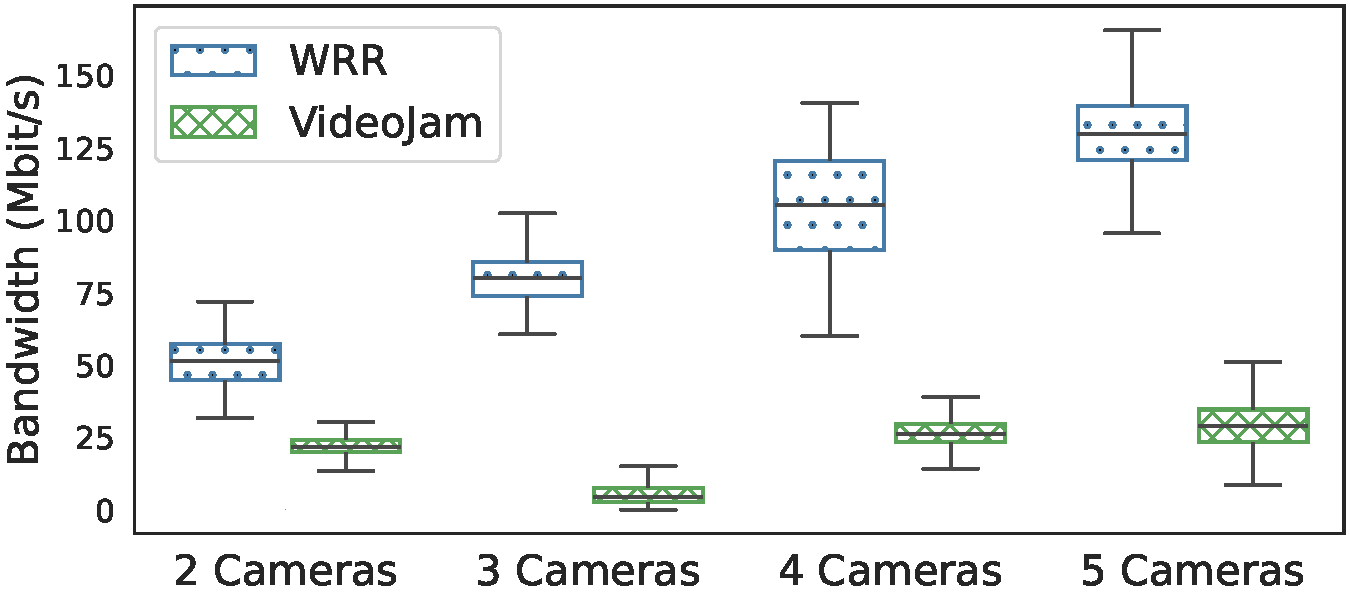
\includegraphics[width=\linewidth]{chapters/videojam/images/agains_weighted_roundrobin/bandwidth.pdf}
		\subcaption{Bandwidth used for offloading to neighbors.}
		\label{fig:against_wrr_bandwidth}
	\end{minipage}
	\vspace{-1mm}
	\caption{Evaluation on several configurations shows the need for a load-balancing technique and the effectiveness of VideoJam in achieving lower response times with less bandwidth usage.}
	\vspace{-3mm}
	\label{fig:against_wrr}
\end{figure*}

\begin{figure}[htb]
	\centering
	\begin{minipage}[t]{.66\linewidth}
		\centering
		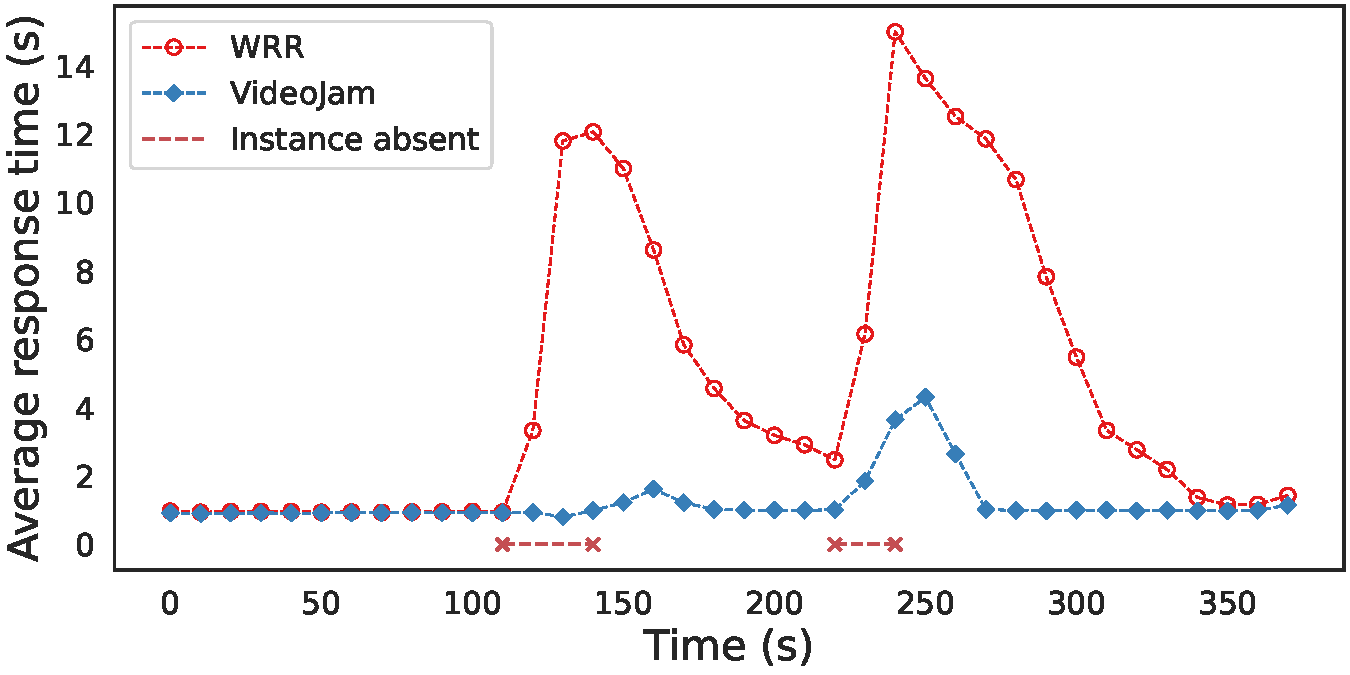
\includegraphics[width=\linewidth]{chapters/videojam/images/adaptability/average_response_time_timeseries.pdf}
		\subcaption{Averages for frames exiting YOLO.}\label{fig:adaptability_avg_response_time}
	\end{minipage}
	% \hfill
	\begin{minipage}[t]{.32\linewidth}
		\centering
		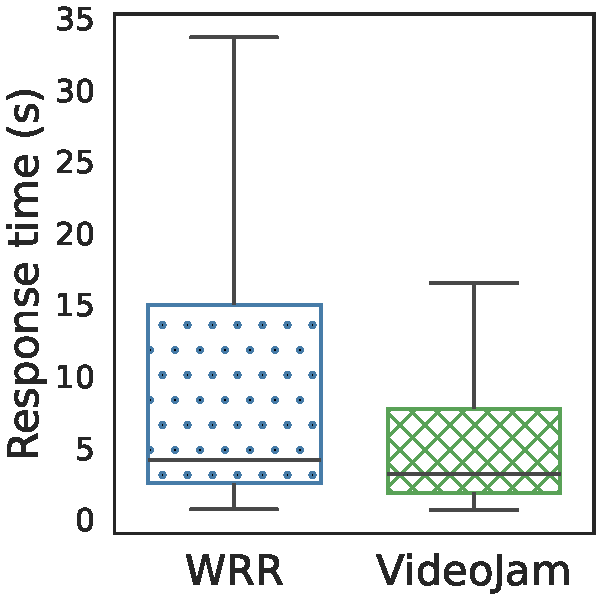
\includegraphics[width=\linewidth]{chapters/videojam/images/adaptability/response_time.pdf}
		\subcaption{Response time.}\label{fig:adaptability_response_time}
	\end{minipage}
	\vspace{-1mm}
	\caption{Evaluation under node failure conditions: WRR's poor performance and VideoJam's adaptability under failures.}
	\vspace{-3mm}
	\label{fig:adaptability}
\end{figure}


\paragraph{VideoJam Under Different Workloads.} To evaluate the sensitivity of VideoJam to the level of workload, we subject it to different workloads, increasing the number of source cameras given a fixed function placement (deployment). In this scenario, we use six GPU-equipped nodes, and we set the number of YOLO and OCR instances to three and five respectively, while we increase the number of mobile cameras from two to five with a rate of 15 frames per second. 

~\Cref{fig:against_wrr} shows the system response time, the percentage of lost frames, and the bandwidth used during the offloading. VideoJam generally shows better performance with respect to the other compared solutions. The poor performance of no-balancing strategy highlights the need of load balancing solutions in this context. WRR reasonably shows longer response times as the load increases since such solution struggles in presence of network congestion. This is also highlighted by the increase in the bandwidth utilization showed in~\Cref{fig:against_wrr_bandwidth}. VideoJam, on the other hand, even in the event of congestion, only offloads the difference between instances to prevent two instances from sending load to each other, which explains the low bandwidth used. Furthermore, given the efficient collaboration among neighbors, VideoJam maintains stable performance as the workload increases.

In summary, this experiment has shown that VideoJam balances the workload without compromising performance, while minimizing system response time. In addition, while WRR statically balances incoming workload to neighbors, VideoJam adapts to the current situation by computing the most appropriate policy, and prevents bandwidth wastage due to bidirectional load migration.



\paragraph{VideoJam's Adaptation to Functions Placement.}
We evaluate the impact of different placement strategies (configurations) on VideoJam, particularly in the case of real-time variations. Note that there is a fundamental difference between workload variations and configuration changes or function placement strategies. Whereas in the previous experiment, we studied workload variation, which applies to the number of objects to be processed in each video stream, in this experiment we will study the case of configuration changes, which applies to the number of streams and processing modules available in the system.

Many studies have been carried out to find a better solution for placing components or functions to maximize the use of hardware resources while maintaining good precision~\cite{201465videostorm,hung2018videoedge}. As VideoJam is agnostic of the placement, we aim to evaluate if performance remains stable across different configurations. To do this, we start with four sources (15fps), three low-resolution YOLOs and five OCRs. First, we deliberately remove a YOLO function before redeploying it, but this time with a higher resolution, but with a higher inference time (lower throughput). This corresponds to a configuration change that can occur when placement techniques are used. In a second step, we kill all components (YOLO and OCR) on another node before restarting them after about 15 seconds. This simulates a node failure that can occur at any time when dealing with edges.

The system response time and the average response time of frames, as they leave the YOLO component, are shown in~\Cref{fig:adaptability_response_time} and~\Cref{fig:adaptability_avg_response_time} respectively. Initially, YOLOs maintain a consistently low response time, as they efficiently handle the incoming workload that is below their capabilities. At $\sim$100s (\Cref{fig:adaptability_avg_response_time}), a YOLO instance fails, with the source previously connected to it now sending its stream to another instance. This results in a sudden increase in the load that is badly distributed between instances for WRR. In contrast, in with VideoJam, instances remain capable of handling all the load generated by the sources. When the function is reintroduced into the system with a different configuration (higher resolution), WRR shows a gradual and slow decrease in response time, as it is unable to redistribute the loads already allocated to instances. 

\begin{figure}[t!]
	\centering
	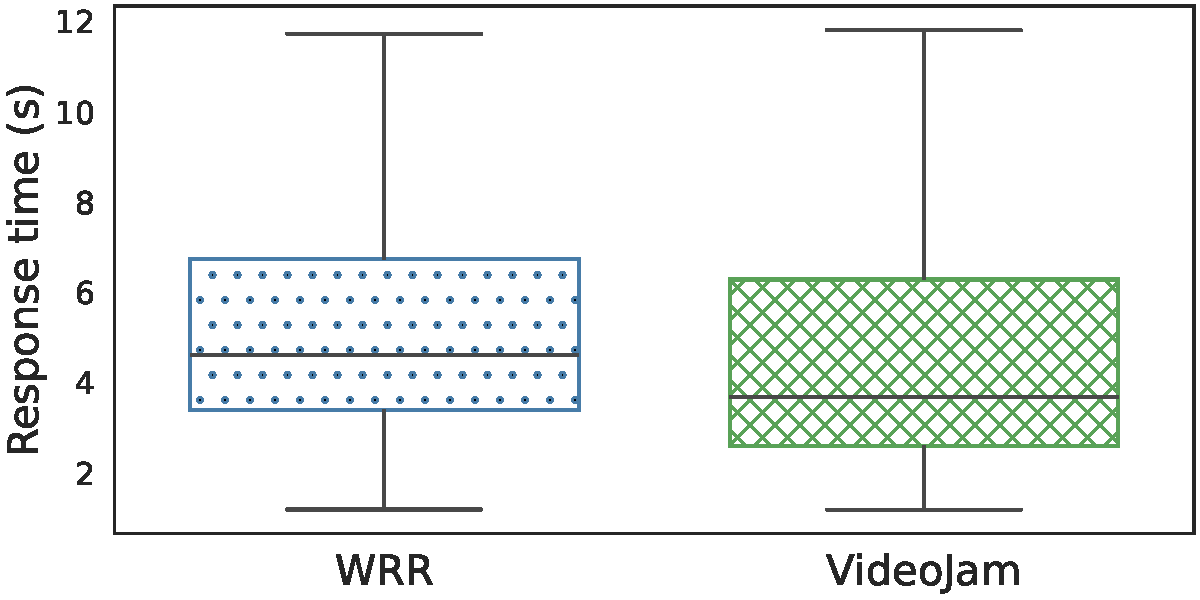
\includegraphics[width=.6\linewidth]{chapters/videojam/images/impact_of_mobility/response_time.pdf}
	\caption{Little effect of source mobility and abrupt flow changes on VideoJam performance.}
	\label{fig:impact_mobility}
\end{figure}

A similar behavior is observed at $\sim$220s, where a YOLO and an OCR deployed in the same node are killed due to node failure. Here again, the response time increases for WRR and VideoJam. In this particular case, the remaining YOLOs (one high-resolution and one low-resolution) are unable to handle the incoming workload, resulting in an increase in response time. In contrast, VideoJam excludes the outgoing instance from the load-balancing policy until it returns, or new functions are added, allowing previously accumulated overload to be efficiently redistributed between instances.


\paragraph{Impact of Mobility.} One of the key features of mobile cameras is their ability to be in the right place to retrieve useful information. We aim to emulate mobile cameras, such as dash cams mounted on cars, entering and leaving the system. We emulate this scenario in our experiment as follows: at first, we have a camera streaming mobile content (\ie, a dash cam content as described in~\Cref{sec:setup}, in the paragraph related to the datasets); after a fixed amount of time, the camera leaves the system, emulating the car leaving the area currently being processed. Finally, a new video starts streaming, emulating a new car entering the system. For the experiment, we used three moving cameras (20fps) which send their streams to four YOLOs, which in turn send them to five OCR instances. At a given time, one camera stops sending its stream to the next function for a short period of $\sim$15 seconds. This represents a camera leaving the system and has a direct impact on the load, as the incoming workload correlation is broken. We observe the system response time in~\Cref{fig:impact_mobility}. When a source stops sending its data stream to the next function, the latter sees its incoming load drop drastically and then fails~VideoJam's prediction. Even though WRR is agnostic to these events as it continues to distribute frames independently of sources, VideoJam's load balancing compensates for eventual forecasting errors, maintaining 1.25$\times$ better response time. 

% Conclusion and Future Work
\section{Conclusion}\label{sec:conclusion}

We present VideoJam, a new approach designed to meet the challenges of video analytics applications that integrate heterogeneous camera sources, \ie, both fixed and mobile. VideoJam responds to scenarios incurring high load variability (such as mobile cameras) by integrating short term load prediction and performing load balancing at function level. Further, the system adapts to varying deployment configurations, not requiring any hard reboots to compensate for them. Thanks to its design, VideoJam reduces response times by 2.91$\times$ lower response time, while reducing video data loss by more than 4.64$\times$  and generating lower bandwidth overheads.

In future work, we plan to tackle the need of accounting of additional constraints in the analytics pipeline. Currently, VideoJam does not consider inter-function link bandwidths to determine load balancing policies. In heterogeneous network environments, where link speeds differ, this omission can have an impact on overall system efficiency. In addition, while VideoJam works independently of the existing deployment configuration (\eg, number of replicas for each function), it does not compensate for scenarios where the load exceeds the existing processing capabilities (\eg, too many video sources to process). Furthermore, it could be interesting to treat neighborhood cases with functions that are not necessarily identical, but rather functions with identical or similar objectives but slightly different implementation (\eg, YOLOv5 and SSD~\cite{liu2016ssd} are similar).~VideoJam, by default, can handle this heterogeneity, although they are treated as identical functions with different performances. However, these functions have many more differences, for example in terms of accuracy, size, inference time, \etc, and therefore raise more challenges.\\
Future work will address these limitations, with the aim of improving resource utilization and exploring more adaptive deployment strategies.

\setchapterpreamble[u]{\margintoc}
\chapter{\roomie{}: Efficient Model Cohabitation in Edge Computing Model Serving}
\label{ch:roomie}

\section{Introduction}\label{sec:intro}

Machine learning (ML) inference serving has become a foundational task for a variety of domains, with organizations  increasingly deploying ML models that applications spanning from computer vision to natural language processing~\cite{}. Unfortunately, the growing demand for ML inference requests is now outpacing hardware availability, creating a critical resource gap that forces organizations to maximize utilization of existing computational infrastructure. To process the incoming data streams in real-time while working within these constraints, scalable model serving architectures have been proposed to support a multitude of applications across video analytics, language understanding, recommendation systems, anomaly detection, and more~\cite{ahmad2024proteus,olston2017tensorflowserving,shubha2024usher,francisco2021infaas,mendoza2021interference}. The increasing data volume demands of state-of-the-art models, coupled with tight \acrlong{slo}s (\acrshort{slo}s) (\eg, latency), has made efficient resource utilization a core challenge across all deployment scenarios.

To address these resource constraints, recent work has explored deploying ML inference pipelines across diverse computational environments, ranging from cloud-grade server clusters to resource-constrained edge devices~\cite{mendoza2021interference,hu2021scrooge,ahmad2024proteus,shubha2024usher,cui2021Abacus,2017clipper}. For instance, cloud platforms like AWS SageMaker or Google Cloud AI offer scalable compute and storage, enabling high-throughput inference for applications such as real-time fraud detection or large-scale recommendation systems. However, these deployments often suffer from network latency and raise data privacy concerns, especially in domains like healthcare or finance where sensitive data must remain local. Conversely, edge deployments—such as running inference on NVIDIA Jetson modules embedded in traffic cameras or smart manufacturing sensors—can reduce latency and mitigate privacy risks by processing data near its source. Yet, these edge devices typically have limited compute and memory, as they are co-located with existing infrastructure like routers or \acrshort{iot} gateways. Regardless of the deployment environment, efficiently managing available resources requires intelligent distribution of inference requests across the infrastructure~\cite{olston2017tensorflowserving,francisco2021infaas}. Unfortunately, existing ML inference serving frameworks, such as TensorFlow Serving or TorchServe, often assume homogeneous, resource-rich environments and overlook the constraints of edge settings, leading to suboptimal hardware utilization and degraded performance.

While significant research has addressed orchestrating model placement and query distribution~\cite{2017clipper,olston2017tensorflowserving,gujarati2020servingdnnslikeclockwork}, these approaches yield limited benefits when the performance profiles of deployed models are imprecisely characterized or when models operate concurrently. This is particularly problematic in resource-constrained environments where multiple models must share limited hardware and can significantly interfere with each other's execution. Recent work such as Usher~\cite{shubha2024usher} attempted to address this gap by analyzing models at the kernel level to better understand performance under interference conditions. However, their approach fails to account for the complex execution patterns of models on \acrshort{gpu} architectures, resulting in inaccurate performance predictions (as discussed in detail in Section~\ref{sec:motivation}). This limitation becomes especially critical in resource-constrained deployment scenarios, where even minor performance estimation errors can dramatically impact overall system efficiency, potentially rendering carefully orchestrated deployments infeasible. A more nuanced understanding of model execution characteristics is therefore essential to enable truly efficient inference serving across all computational environments.

In this paper, we present~\roomie{}, a model serving orchestration architecture that maximizes system performance in scenarios where colocation is necessary across resource-constrained environments.~\roomie{}'s key contribution is its kernel-aware interference profiling that captures the sequential nature of \acrshort{gpu} kernel execution patterns when multiple models share hardware resources. By understanding how specific kernel sequences from different models interact,~\roomie{} builds accurate interference profiles that predict performance degradation under various colocation scenarios. This fine-grained approach enables~\roomie{} to make better informed placement decisions, identifying which models can efficiently coexist on the same hardware and which combinations should be avoided to maintain performance across both goodput and latency.

Our experimental evaluation demonstrates~\roomie{}'s effectiveness across a diverse set of inference models and deployment scenarios. In cloud deployments,~\roomie{} achieves up to 17× lower latency and sustains over 97\% processing rate, outperforming state-of-the-art solutions~\cite{shubha2024usher,francisco2021infaas} through interference-aware colocation and resilience to saturation. On edge devices, it maintains up to 9× lower response times and 1.5× higher throughput, effectively navigating resource constraints. These improvements come from~\roomie{}'s smart scheduling, which stays close to the best possible setup even under high concurrency. By precisely characterizing interference patterns and adapting to system dynamics,~\roomie{} enables scalable, high-efficiency inference serving across modern \acrshort{gpu} platforms.

\section{Motivation and Challenges}\label{sec:motivation}


In this section, we will discuss the importance of taking model interference into account when inference serving, as demonstrated by the suboptimal performance of existing approaches.

\begin{figure}
	\centering
	\begin{subfigure}[t]{0.45\textwidth}
		\centering
		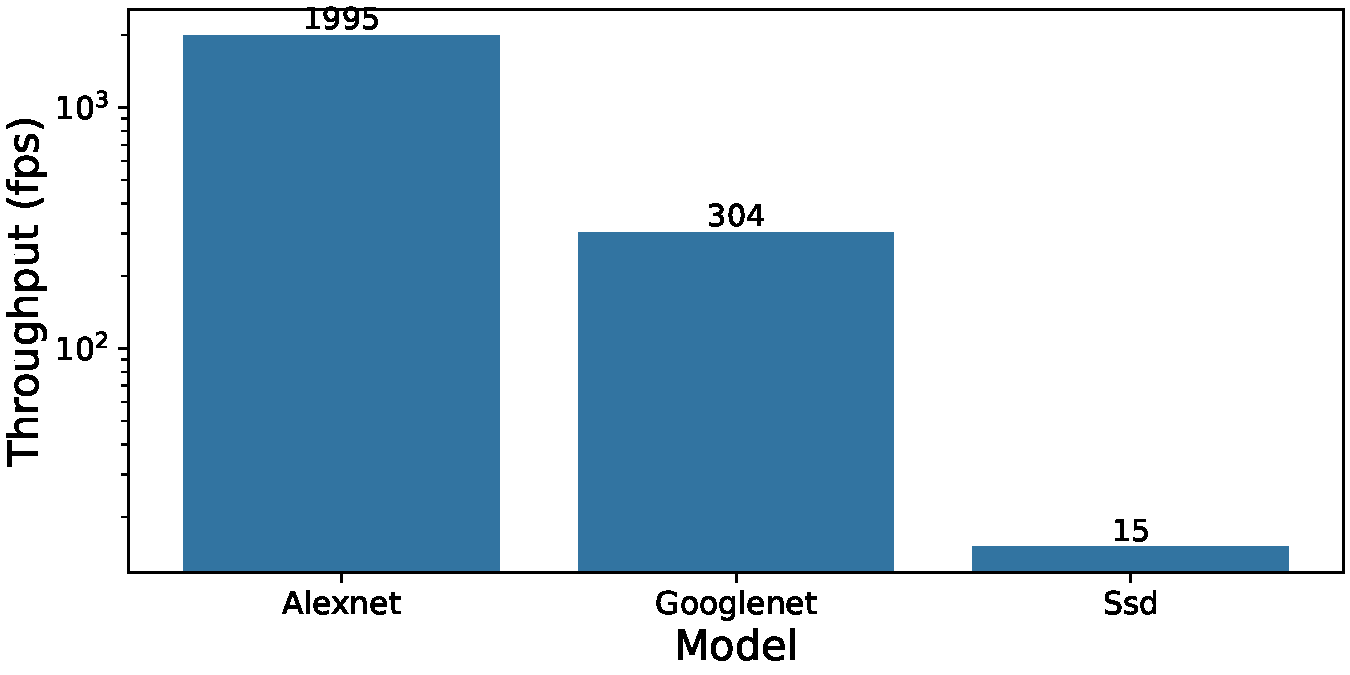
\includegraphics[width=\textwidth]{chapters/roomie/images/Throughput_models_in_isolation.pdf}
		\caption{Throughput when the model operates in isolation, without any interference.}
		\label{fig:isolation}
	\end{subfigure}
	\hfill
	\begin{subfigure}[t]{0.45\textwidth}
		\centering
		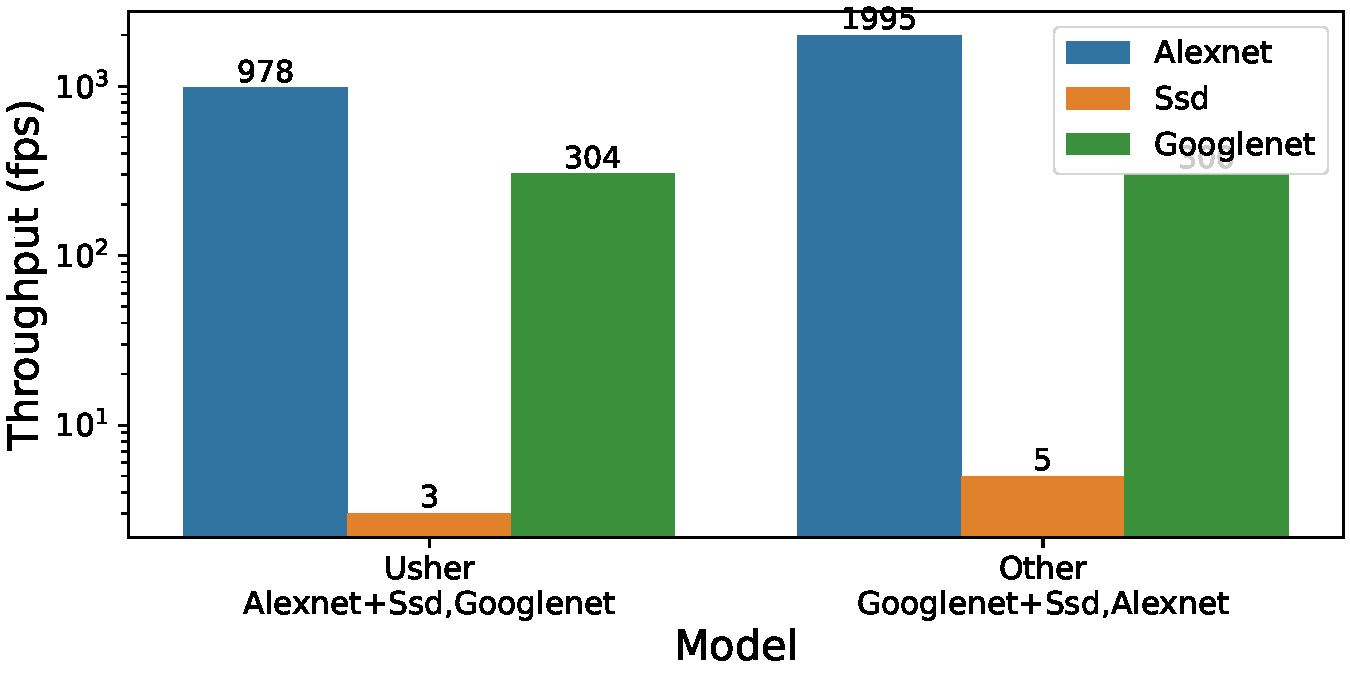
\includegraphics[width=\textwidth]{chapters/roomie/images/Throughput_models_in_combinaison.pdf}
		\caption{An alternative to co-locating three models on two GPUs, offering a better compromise than Usher~\cite{shubha2024usher}.}
		\label{fig:colocation}
	\end{subfigure}
	\label{fig:three graphs}
\end{figure}

\subsection{Limitations of Existing Inference Serving Strategies}

The deployment of machine learning models for inference serving has become increasingly critical across domains such as computer vision, natural language processing, and recommendation systems. As demand for real-time inference grows, organizations are compelled to maximize the utilization of existing computational infrastructure, particularly in resource-constrained environments. While scalable serving architectures have been proposed to meet service level objectives (SLOs), such as latency and throughput, many existing systems rely on simplistic heuristics for model placement and colocation. These approaches typically reference offline profiling data or prioritize devices with the most available memory, overlooking the nuanced performance degradation that arises when multiple models share GPU resources.

The assumption that memory availability is a reliable proxy for inference performance is mistaken. During inference, models consume significantly less memory compared to training, as intermediate states and gradients are not retained. Consequently, memory-centric placement decisions fail to account for the dynamic interference between concurrently executing models. Systems such as Usher attempt to address this by analyzing low-level GPU kernels to estimate resource demands. However, their methodology does not capture the complex interactions between kernels from different models, leading to suboptimal colocation choices.

We conducted an experimental study to evaluate the performance of three inference models: AlexNet, GoogLeNet, and SSD, on two Jetson Xavier devices. The performance of each deep neural network (DNN) when operating in isolation is illustrated in~\Cref{fig:isolation}. Our primary objective was to identify the optimal co-location configuration among all possible combinations. Our findings revealed that Usher's proposed approach of co-locating AlexNet with SSD is not necessarily the most effective option. In fact, an alternative configuration, GoogLeNet paired with SSD—demonstrates a superior balance in performance (refer to Figure colocation).

We have determined that Usher's misjudgment stems from the method used to assess model compatibility. Merely classifying models based on their computing or memory capacity does not provide a comprehensive understanding of their performance. A more nuanced approach that considers the resource demands of each model over time is essential for accurate evaluation.


\subsection{The Importance of Kernel-Level Analysis}

Deep neural networks (DNNs) perform inference by executing a sequence of GPU kernels, each responsible for specific low-level computations and defined by distinct resource requirements such as shared memory, register usage, and execution time. These kernels, rather than the high-level model architecture, constitute the true computational footprint on the GPU. Profiling tools such as Nsight Systems~\cite{nsight_systems} and Torch Profiler~\cite{torch_profiler} enable fine-grained observation of kernel behavior, revealing patterns of resource occupancy and execution timing that are often obscured at the model level. Empirical analysis shows that individual kernels frequently leave portions of the GPU underutilized, suggesting that with careful orchestration, multiple models can be deployed simultaneously to improve overall throughput.

However, when models are executed concurrently on the same GPU, their kernels may overlap in time and compete for limited hardware resources. Although this parallelism can enhance utilization, it also introduces a critical challenge: interference. This occurs when the combined resource demands of overlapping kernels exceed the GPU's capacity, forcing the hardware to serialize execution or delay kernel launches. For instance, if two kernels simultaneously require more shared memory or registers than the GPU can allocate, contention arises, leading to extended execution times and degraded performance. The severity of interference is shaped not only by the type of resources consumed but also by the duration and temporal alignment of kernel execution. Without precise modeling of these interactions, colocation decisions risk undermining system efficiency rather than enhancing it.

Effective colocation requires more than simply identifying underutilized resources; it demands a precise understanding of how kernels from different models interact during concurrent execution. The configuration of each kernel (its use of shared memory, registers, and other architectural resources) determines its potential for interference with others. Predicting these interferences cannot be based solely on aggregated model statistics or layer-level abstractions, as these overlook the fine-grained execution dynamics that govern actual performance. Instead, kernel-level analysis must consider both static resource requirements and temporal execution behavior to assess how overlapping workloads compete for limited GPU capacity. By modeling these interactions, it becomes possible to identify model pairs that minimize conflicts and make informed colocation decisions that preserve throughput and latency under constrained conditions.

\subsection{Challenges in Modeling and Predicting Interference}

% \begin{figure}
% 	\centering
% 	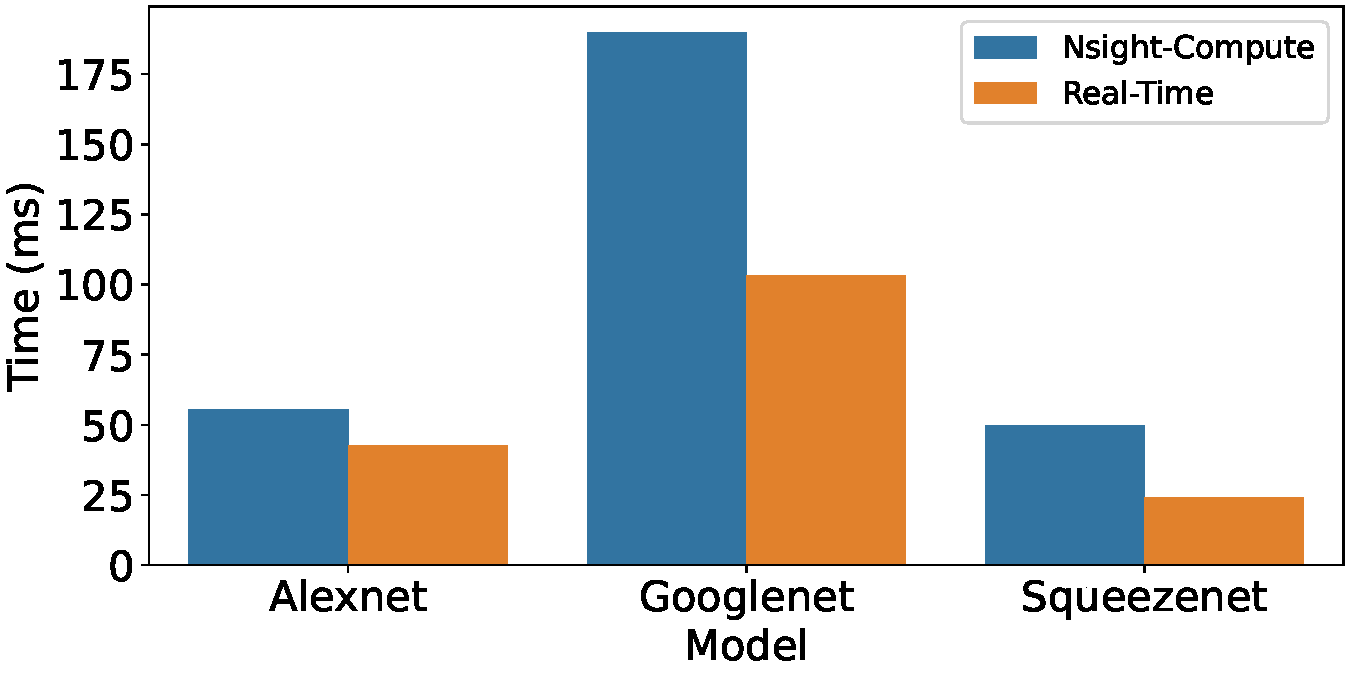
\includegraphics[width=\textwidth]{chapters/roomie/images/duration_gap.pdf}
% 	\caption{Throughput when the model operates in isolation, without any interference.}
% 	\label{fig:duration_gap}
% \end{figure}

Determining the best colocation strategy for deep neural networks (DNNs) sharing a GPU requires a nuanced understanding of how their kernels interact during inference. The goal is to identify model pairings that maximize throughput and minimize latency by avoiding harmful interference. Achieving this demands accurate performance modeling at the kernel level, where resource contention and execution overlap directly impact runtime behavior. However, building such models introduces several practical and computational challenges that must be addressed to ensure scalability and reliability.

\paragraph{Profiling overhead and trace collection.}
% Profiling is essential for capturing the fine-grained execution characteristics of DNN kernels, including resource usage and execution time. These metrics form the backbone of any interference-aware colocation strategy. Yet, collecting accurate traces is inherently time-consuming and introduces overhead that can distort the very measurements it seeks to record. Profiling tools rely on instrumentation and callbacks that add latency to kernel execution, often resulting in total recorded durations that exceed the actual inference time. This discrepancy complicates performance estimation and can mislead scheduling decisions if left uncorrected. Despite these limitations, profiling remains indispensable, as predicting kernel behavior analytically is highly challenging due to the variability in runtime configurations and hardware-specific optimizations. Fortunately, the process can be made tractable by profiling models in isolation. Since the number of GPU architectures in deployment is relatively small, and many models follow standardized execution patterns, it is feasible to build a reusable profiling database that supports accurate interference modeling without incurring prohibitive cost.
% Profiling is crucial for capturing the detailed execution characteristics of Deep Neural Network (DNN) kernels, particularly regarding resource usage and execution time, which are essential for interference-aware colocation strategies. However, the process of collecting accurate execution traces is time-consuming and introduces overhead that can distort measurements, often resulting in recorded durations that exceed actual inference times. This discrepancy complicates performance estimation and may mislead scheduling decisions if uncorrected. Despite these limitations, profiling is indispensable, as predicting kernel behavior analytically is challenging due to variability in runtime configurations and hardware-specific optimizations. Profiling models in isolation can alleviate some of these issues, and given the relatively small number of GPU architectures in use and the standardized execution patterns of many models, it is feasible to create a reusable profiling database that supports accurate interference modeling without incurring prohibitive costs.
Profiling is essential for capturing the fine-grained execution characteristics of DNN kernels, including resource occupancy and duration. These metrics form the backbone of any interference-aware colocation strategy. Yet, collecting accurate traces is inherently time-consuming and introduces overhead that can distort the very measurements it seeks to record. Profiling tools rely on instrumentation and callbacks that add latency to kernel execution, often resulting in total recorded durations that exceed the actual inference time.
In practice, we observed that the ratio between profiled kernel durations and actual inference time can vary considerably, sometimes exceeding the true runtime by a wide margin, highlighting how profiling overhead may distort performance measurements and must be carefully considered.
% This discrepancy complicates performance estimation and can mislead scheduling decisions. Figure~\ref{fig:duration_gap} illustrates this phenomenon, showing the gap between the measured inference time and the aggregate kernel durations.
Despite these limitations, profiling remains indispensable, as predicting kernel behavior analytically is highly challenging due to the variability in runtime configurations and hardware-specific optimizations. What's more, cuDNN~\cite{cudnn} provides highly tuned implementations for standard routines such as convolution, attention, matrix multiplication, pooling, and normalization. For the same operator type, it may execute different kernels depending on the GPU architecture and available resources, with varying configurations in register usage, shared memory, and execution strategy. While this process is time-consuming, it remains feasible due to the limited number of GPU variants and the ability to profile models only in isolation.

\paragraph{Combinatorial Complexity of Kernel Overlap Scenarios.}
% Another significant challenge lies in modeling the overlapping execution of kernels across multiple DNN models. While the analytical framework developed earlier enables estimation of interference effects, applying it exhaustively is computationally prohibitive. Real-world deployments do not guarantee synchronized kernel execution; instead, each model may begin inference from any point in its kernel sequence. Evaluating all possible alignments requires constructing a full Cartesian product of starting indices, resulting in exponential growth in the number of scenarios as the number of models increases. This combinatorial explosion makes real-time evaluation impractical.
A key challenge in optimizing deep neural network colocation lies in defining and identifying the interference itself. Interference is not a static property: it arises dynamically when the kernels of different models overlap during execution and compete for shared GPU resources. To determine which kernels are likely to interfere, it is necessary to analyze not only their resource requirements, but also their temporal alignment and execution context. This is particularly difficult because interference depends on both the type and timing of resource usage, which can vary across deployments and hardware configurations.\\
This challenge is compounded by the vast number of possible overlapping scenarios. In realistic service environments, models do not begin inference in a synchronized manner; each can start at any point in its kernel sequence, leading to a vast space of potential execution alignments. Taking into account all combinations of starting positions across multiple models leads to exponential growth in the number of scenarios as the number of models increases. This combinatorial explosion makes exhaustive evaluation impractical for real-time decision-making. The challenge lies in estimating the impact of interference without simulating all possible alignments, while maintaining sufficient fidelity to guide effective colocation strategies.

To support efficient colocation of deep neural networks on shared GPUs, we introduce~\roomie, a kernel-level profiling and interference estimation strategy that balances precision with scalability. By analyzing execution traces in isolation and simulating representative overlap scenarios,~\roomie{} enables informed deployment decisions without incurring prohibitive computational cost.



% Modeling kernel interference presents several challenges. First, the diversity of GPU architectures and model types necessitates extensive offline profiling to capture performance characteristics across deployment scenarios. While this process is time-consuming, it remains feasible due to the limited number of GPU variants and the ability to profile models in isolation. Second, predicting interference requires identifying which kernels will overlap in execution and assessing the impact on their runtime. This involves analyzing resource contention at a granular level, including shared memory and register usage, and determining whether the combined demand exceeds the GPU's capacity.

% Furthermore, the execution order of kernels and their serialization within CUDA streams influence the degree of interference. Kernels with complementary resource profiles may coexist with minimal performance degradation, while those with overlapping demands can significantly delay each other's execution. Existing approaches that rely solely on layer-level information or aggregate model statistics fail to capture these subtleties. Therefore, a more refined methodology is required—one that profiles kernels individually, models their interactions, and predicts the resulting performance impact under colocation. Addressing these challenges is essential for enabling efficient inference serving in environments where computational resources are limited and colocation is unavoidable.

\section{Related Work}\label{sec:related}

With the proliferation of deep learning-based applications offered as online services, managing and scheduling large-scale inference workloads in GPU data centers has become increasingly critical. Unlike resource-intensive training workloads, inference tasks have distinct characteristics that require specialized scheduling solutions. The objectives of inference scheduling (accuracy, latency, and cost-effectiveness) are closely linked. Accuracy efficiency involves selecting the most suitable model for each query and allocating resources intelligently. Latency efficiency requires meeting response time constraints, even in the face of irregular or fluctuating loads. Cost efficiency aims to minimize financial expenditure, particularly in public cloud environments. These objectives are often contradictory, requiring flexible and comprehensive planning systems capable of balancing trade-offs between different performance dimensions.

\paragraph{Inference Serving Systems.}
Several systems have been proposed to address the challenges of inference scheduling. Clipper~\cite{2017Clipper} supports multiple ML frameworks and simplifies model deployment for real-time applications, but does not account for resource interference. TensorFlow-Serving~\cite{olston2017tensorflow} adapts to traffic changes by scaling replicas, yet similarly overlooks interference among colocated models. Clockwork~\cite{gujarati2020servingDNNlikeclockwork} offers predictable performance by executing one inference at a time with full GPU capacity, but this design underutilizes GPU resources due to limited concurrency. Proteus~\cite{ahmad2024proteus} introduces adaptive batching and dynamic model variant selection to optimize throughput and accuracy. However, its restriction of one model variant per device limits co-location and parallel execution, leaving GPU resources underexploited.

\paragraph{Multi-Tenant DNN Inference on Shared GPUs.}
To improve resource utilization, recent work has explored concurrent execution of multiple models on shared GPUs. INFaaS~\cite{francisco2021infaas} enables model-less serving by dynamically selecting variants based on query load and performance constraints. It co-locates variants and scales workers reactively, but struggles with profiling complexity and lacks proactive interference prediction. Colti~\cite{mobin2023colti} enhances throughput by colocating models for training and inference. Yu et al.~\cite{yu2021automated} exploit operator-level independence to schedule concurrent execution across streams, reducing latency. REEF~\cite{han2022microsecond} supports kernel preemption and priority-based sharing to maintain predictable performance. Miriam~\cite{zhao2023miriam} introduces elastic kernels for real-time prioritization, enabling flexible scheduling across tasks with varying criticality. While these systems optimize post-deployment execution, they often neglect initial placement strategies that could preemptively mitigate interference.

\paragraph{Interference-Aware Inference Serving.}
Recent studies have focused on proactive scheduling by modeling and predicting interference between concurrently running models. Mendoza et al.~\cite{mendoza2021interference} propose a latency degradation model based on global buffer and PCIe utilization, but the coarse granularity limits predictive accuracy. Scrooge~\cite{hu2021scrooge} profiles concurrency thresholds for identical DNNs to determine optimal co-location, yet its approach is infeasible for heterogeneous model combinations due to profiling overhead. Abacus~\cite{cui2021Abacus} schedules operators from multiple models jointly to maintain QoS, but its hardware-agnostic duration model and reactive execution lead to underutilization and increased latency. iGnifer~\cite{xu2023iGniter} adopts a low-level perspective, using GPU metrics such as L2 cache usage and core launch counts to characterize interference. However, coarse indicators like power consumption prove less predictive. Usher~\cite{shubha2024usher} refines interference modeling by analyzing kernel occupancy and DRAM usage, distinguishing between compute- and memory-intensive workloads. Both Usher and iGnifer rely on NVIDIA's Multi-Process Service (MPS)~\cite{nvidiaMPS575} for spatial sharing, which limits their applicability in edge environments such as NVIDIA Jetson, where MPS is unsupported.

\section{Kernel Interference-Aware Scheduling}\label{sec:kernel_interference_aware_scheduling}
This section explains the main concept behind~\roomie. First, we introduce the idea of interference and describe a method for estimating it. Next, we present an algorithm that efficiently calculates the interference among various models. Finally, we detail a placement algorithm that utilizes the interference estimation from the first procedure to efficiently allocate new incoming models to the available GPUs.

\subsection{Kernel Interference Estimation}

% When a new request arrives, you must perform two actions: choose a variant and select the resource in which to deploy it. Several strategies can be used to choose a variant. You can choose the fastest variant for a time-constrained application, or the most accurate but potentially slower variant. This information is often obtained by profiling the model off-line.

%Kernel-level interference takes into account the interference that the kernels of several models deployed on the same GPU resource may have with each other. 
%When a model is running for inference on an NVIDIA GPU, it launches a sequence of kernels for each of its layers. A kernel represents a single operation executed by many threads in parallel. Each kernel is launched with a configuration that defines the size of the kernel grid, the division of the grid into blocks and the GPU resources required (\eg, registers per thread, shared memory per block) to execute the kernel. A grid is an array of thread blocks. % and a block represent a 1D, 2D or 3D array of threads. \ff{Not clear, what is a grid? We should be more detailed here and add more references.} 
%Threads within a block can share memory and synchronize their execution. Choosing an efficient launch configuration maximizes device utilization. A group of 32 threads within a cooperative thread arrays (CTAs) or blocks is called warps. A streaming multiprocessor (SM) handles execution of a kernel as groups warps. Blocks are the basic units of execution on the GPU and are scheduled to run on the multiprocessors of the GPU. Each block is given a certain amount of shared memory and a maximum number of threads it can contain, which is hardware-dependent.

%The execution resource demands of individual threads ultimately constrain the maximum number of threads that can be active (running) simultaneously. There are multiple hardware limitations such as the maximum number of threads per block, the maximum registers per thread, maximum registers per block, just to name some. While exceeding some of these limitations will prevent the kernel from executing like the maximum registers per thread, others prevent the kernel from using all resources that will be in its disposable. When a kernel is limited by the number of warps that can be active at the same time in a SM this is characterized as limited by warps. A kernel is limited by registers when the number of registers per thread exceed total registers available per multiprocessor. A kernel is memory limited when the amount of shared memory available per multiprocessor limits the number of blocks that can be active at the same time. 
%Many other limitations might also prevent a kernel from full using GPU resources such as memory bandwidth of the GPU necessary for transferring data GPU memory and the multiprocessors. Therefore, the occupancy is the ratio of the number of active warps per multiprocessor to the maximum number of possible active warps. The theoretical occupancy can be calculated offline and represents the upper limit of occupancy imposed by the kernel launch configuration and the capabilities of the CUDA device~\cite{lim2017autotuninggpukernelsstatic}. On the other hand, the achieved occupancy is measured during kernel execution and represent actual occupancy of the GPU.

% With that knowledge, when two kernels are executed at the same time, warp schedulers responsible for scheduling warps can schedule different warps from different kernels to run in parallel when the hardware resource allows it.

% Then kernel level interference would be the effectiveness of leveraging the insight of kernel execution and exploiting that to determine how multiple kernels might interference one other. In fact, when kernels have different limitations that can eventually lead the possible of running multiple of them at the same time. However, when kernels from different models at a specific time are requested for execution, there will be interference if on prevent another from reaching it previously preditermined occupancy. In other words, si un kernel avait au départ une certaine occupancy et que ce dernier doit partager les resources disponibles avec un autre kernel et que celui-ci reduit some nombre de block as explained previously, then this kernel will be considered in interference. And the performance drop can be computed according to the new occupancy.
% Understanding how kernels execute is crucial for recognizing how they can interfere with one another. Interference happens when one kernel prevents another from reaching its intended performance level while both are scheduled to run simultaneously. In simpler terms, interference occurs when the demand for resources from multiple kernels at the same time exceeds the total resources that the GPU can provide. If a kernel is designed to operate at a certain capacity but must share resources with another kernel, it may end up with fewer resources available for its tasks. In this case, we say the kernel is experiencing interference. This interference can lead to lower performance, which can be measured by determining the new kernel achievement, i.e., occupancy. And this new achievement can be used to determine the new execution time of the kernel, as it may take longer to complete its tasks with fewer resources. We will demonstrate that accurately estimating this interference at the kernel level is essential for effectively managing the allocation of new models on GPUs, as it allows for better resource distribution and improved overall performance.

Understanding how kernels execute is crucial for recognizing how they can interfere with one another. Interference happens when one kernel prevents another from reaching its intended performance level while both are scheduled to run simultaneously. In simpler terms, interference occurs when the demand for resources from multiple kernels at the same time exceeds the total resources that the GPU can provide. If a kernel is designed to operate at a certain capacity but must share resources with another kernel, it may end up with fewer resources available for its tasks. In this case, we say the kernel is experiencing interference.
This interference can lead to lower performance, which can be measured by determining the kernel's new achievement, specifically its occupancy. This new occupancy can then be used to estimate the kernel's execution time, as it may take longer to complete its tasks with fewer resources. We will demonstrate that accurately estimating this interference at the kernel level is essential for effectively managing the allocation of new models on GPUs, as this helps to improve overall performance.

%would be the effectiveness of exploiting knowledge of kernel execution to determine how multiple kernels can interfere with each other and how to measure the degree of interference. 

\paragraph{Model kernels.}

When a model runs inference on an NVIDIA GPU, each layer is executed by launching one or multiple kernels, a computational routine that runs in parallel across many threads. These threads are grouped into warps, typically sets of 32 threads that execute instructions in lockstep. Warps ($W$) themselves are organized into blocks ($b$), which serve as the basic scheduling units on the GPU. Blocks are assigned to streaming multiprocessors (SMs), the core computational engines that execute instructions and manage local resources such as registers and shared memory. The efficiency of each kernel depends on how it uses GPU resources, such as registers allocated per thread and shared memory available during execution. While the full execution model involves additional structural details, we focus here on threads, warps, blocks, and resource usage to highlight the core mechanisms relevant to performance. For a comprehensive description of the CUDA execution model, refer to the official documentation~\cite{nvidia2025cuda}.

From this understanding of kernel execution, we can determine its theoretical occupancy, which reflects how many warps are active relative to the hardware's capacity by the following equation :

\begin{equation}\label{eq:occupancy}
	o = \frac{W_b \times b}{W}
\end{equation}
,where $W_b$ is the number of warps per block, $b$ is the number of blocks assigned to an SM, and $W$ is the maximum number of warps the SM can support.

This value provides an overview of the number of active tasks in relation to the hardware's capacity to execute them simultaneously. It is called theoretical utilization because it represents the optimal scenario in terms of the GPU's potential workload. However, it does not guarantee that the kernel will operate efficiently. For a thorough understanding of how it is calculated, please refer to the source in~\cite{lim2017autotuninggpukernelsstatic}.

\paragraph{Kernel Interference.} We characterize a GPU by its capacity $\Phi$, which encompasses hardware limits such as the maximum number of warps, the size of the register file, and the amount of shared memory available per streaming multiprocessor (SM). These resources constrain the execution of a kernel, e.g., the maximum number of warps, the size of the register file, or the shared memory per multiprocessor~\cite{lim2017autotuninggpukernelsstatic}. For a set of kernels $K$ launched to run on the same GPU, interference occurs when the total resource demand exceeds the device's capacity. More formally,

\begin{equation}\label{eq:occurrence}
	\sum_{k \in K} \varphi_k > \Phi
\end{equation}
,where $\varphi_k$ (e.g., warps, registers, and shared memory) denotes the resource usage of kernel $k$, and $K$ is the set of active kernels.

\paragraph{Interference Modeling via Theoretical Occupancy Adjustment.} The main challenge lies in estimating the interference each kernel experiences when executed alongside others. This depends on how the theoretical occupancy is recalculated relative to the capacity of the GPU resources $\Phi$. Since GPU resources are shared among concurrent kernels, they can be redistributed in different ways, and each allocation yields a different occupancy outcome. Various strategies are possible: equal distribution, first-come-first-served, or allocation based on priorities. Each of these affects the amount of resources allocated to the kernel and its performance. Given that the available resources constrain the maximum number of blocks a kernel can launch, we can compute a new maximum blocks $\tilde{b}_k$ for each kernel $k$, based on the redistribution of the GPU resources $\Phi$. For details on this calculation, refer to~\cite{lim2017autotuninggpukernelsstatic}, or consult the implementation provided in our open-source code.

With the new block limit $\tilde{b}_k$, we can derive the new occupancy $\tilde{o}_k$ using the same formulation as in~\Cref{eq:occupancy}. This allows us to estimate the new execution time of the kernel under interference:

\begin{equation*}
	\tilde{d}_k = d_k \times \frac{o_k}{\tilde{o}_k}
\end{equation*}
, where $d_k$ is the execution time of kernel $k$ when running in isolation. Worth mentioned that, if $o_k = \tilde{o}_k$, then no interference occurs, and $\tilde{d}_k = d_k$.

% Interference ends once the first kernel completes its execution. Assuming at most two kernels are interfering, we define the interference period as the time required for the first kernel $k^*$ to finish, $\Delta = \min \left\{ \bar{d}_k \right\}_{\forall k \in K}$.

% \begin{equation*}
% 	\bar{d}^{'}_k = \left(\bar{d}_k - \Delta \right) \times \frac{\tilde{o}_k}{o_k}
% \end{equation*}

Interference ends once the first kernel completes its execution. Assuming at most two kernels are interfering, the remaining kernel continues alone without interference. We define the interference period as the time required for the first kernel to finish, $\Delta = \min \left\{ \tilde{d}_k \right\}_{\forall k \in K}$.
For the remaining kernel, its total duration is composed of two phases: the initial interference period $\Delta$, during which it runs with reduced occupancy $\tilde{o}_k$, and the remaining portion of its execution, which proceeds at full occupancy $o_k$. To account for the change in execution speed, we adjust the remaining time accordingly. Specifically, the portion $\tilde{d}_k - \Delta$, originally computed under reduced occupancy, is scaled by $\frac{\tilde{o}_k}{o_k}$ to reflect the normal execution once interference ends. Formally expressed:

\begin{equation}
	\tilde{d}_k =
	\begin{cases}
		\tilde{d}_k & \text{if } \tilde{d}_k \leq \Delta \\
		\Delta + \left( \tilde{d}_k - \Delta \right) \times \frac{\tilde{o}_k}{o_k} & \text{otherwise}
	\end{cases}
\end{equation}

% \begin{equation}
% 	\tilde{d}_k=
% 	\begin{cases}
% 		k_{i\omega}/k_{p\omega}=2\pi\times 10 \\
% 		\left\lvert\frac{k_{p\omega}s+k_{i\omega}}{s}\cdot\frac{1}{Ts+1}\right\rvert_{S=\mathrm{j}\cdot2\pi}=1
% 	\end{cases}\,.
% \end{equation}

This unified notation allows us to express the adjusted duration for all kernels, whether they complete during the interference window or continue beyond it.

\paragraph{Performance Drop.} Now that we have established a method for estimating interference among simultaneously executing kernels, we can generalize this approach to the inference phase of multiple DNNs. Each DNN launches a sequence of kernels, and we begin by aligning the first kernel of each DNN to form an initial set of concurrently executing kernels. This set is evaluated using the interference model described above. Once the first kernel in the set completes, it is replaced by the next kernel from the same DNN, and the process continues iteratively until all models have completed their execution, that is, until all final kernels have been processed.

For a model with an original inference time $T$ and a total of $q$ kernels, the new inference time under interference is given by:
\begin{equation*}
	\tilde{T} = \sum_{i=1}^{q} \tilde{d}_{k_i}
\end{equation*}

The performance drop experienced by model $m$ due to interference is quantified by the relative increase in inference time. This is computed as:
\begin{equation}\label{eq:performance_drop}
	\mu = \frac{\sum_{i=1}^{q} (\tilde{d}_{k_i} - d_{k_i})}{\sum_{i=1}^{q} d_{k_i}} = \frac{\tilde{T} - T}{T}
\end{equation}

This formulation captures the cumulative slowdown introduced by resource contention across all kernels in the model's execution pipeline.

% Performance Drop. Now that we have an idea of how we can determine interference between multiple simultaneous kernels, we can generalize this to all kernels that simultaneous DNNs launch during the inference of multiple DNNs. We could first align the kernels of each DNN and form a first set of kernels that would run simultaneously and follow the above formulation. Then, the first kernel to finish in this set would be replaced by the next kernel of the DNN to which it belongs. We continue in this manner until all models are completed, i.e., until all the last kernels are reached. After that, a model with an initial inference time $T$ and a total of $q$ kernels would have a new inference time:

% \begin{equation*}
% 	\tilde{T} = \sum^{q}_{i=1} \tilde{d}_{k_i}
% \end{equation*}

% Finally, the performance drop caused by the interferences on a given model, is given by the increase of the inference time, \ie, the sum of kernels' new durations after interference. The performance drop of the model $m$ is determined as:
% \begin{equation}\label{eq:perfDrop}
% 	\mu = \frac{\sum^{q}_{i=1} (\tilde{d}_{k_i} - d_{k_i})}{\sum^{q}_{i=1} d_{k_i}} = \frac{\tilde{T} - T}{T}.
% \end{equation}



% =========



% To estimate the interference within a group of models deployed on a GPU, we need to determine the interference between the kernels of the different models. Given the set of kernels $K_t$ at a particular time $t$ launched by each model on a GPU, the interference will consist in re-distributing the GPU resources $\Phi$ among all the different kernels in $K_t$. We represent with $\bar{\varphi}_k$ the maximum resource allocable to kernel $k \in K_t$ after the re-distribution according to one of the strategies described before.


% We denote by $M$ the set of models deployed on the GPU. Each model $m \in M$ launches a set of kernels $K_m$ for inference. Each kernel $k \in K_m$ is characterized by its duration $d_k$ (in terms of $ms$ or $ns$), its theoretical occupancy $occ_k \in \left[ 0,\, 1\right]$, and required resources $\varphi_k$ (that can be in terms of warps, registers, and shared memory). The theoretical occupancy $occ_k$ represents the highest level of GPU resource utilization that kernel $k$ can achieve during execution. It is calculated as the ratio of active warps per streaming multiprocessor (SM) to the maximum number of warps that the SM can support. Additionally, it reflects the maximum number of thread blocks that can run concurrently, which is constrained by the availability of wraps, registers, or shared memory~\cite{lim2017autotuninggpukernelsstatic}~\footnote{In our code is also available the implementation of the calculation of the theoretical GPU occupancy}. For a given kernel $k$, we represent with $b_k$ its maximum number of allocable blocks.

% The inference time for model $m$ deployed the GPU is defined as:
% \begin{equation}\label{eq:infTime}
% 	T_m= \sum_{k\in K_m} d_k
% \end{equation}
% Each model launches at most one kernel at time $t$, and we represent all kernels launched at that time by each model on the same GPU as $K_t$.

% We define the \textit{occurrence of interference} among kernels in $K_t$ when the sum of the requested resources exceeds the limits of the GPU device. More formally,
% \begin{equation}\label{eq:occurrence}
% 	\sum_{k \in K_t} \varphi_k > \Phi.
% \end{equation}

% In the event of interference, available resources are shared, leading to an increase in the execution time of kernels launched on the GPU. For the re-distribution of GPU resources to kernels in $K_t$, different strategies can be considered. For example, GPU resources can be equally distributed to all kernels in $K_t$, or each kernel can receive a potion of GPU resource proportionally to its demand. Alternatively, priorities strategies can be applied, such as First-Come First Served (FCFS), where resources are assigned to the kernel with the highest priority.

% \paragraph{Interference estimation} To estimate the interference within a group of models deployed on a GPU, we need to determine the interference between the kernels of the different models. Given the set of kernels $K_t$ at a particular time $t$ launched by each model on a GPU, the interference will consist in re-distributing the GPU resources $\Phi$ among all the different kernels in $K_t$. We represent with $\bar{\varphi}_k$ the maximum resource allocable to kernel $k \in K_t$ after the re-distribution according to one of the strategies described before.

% Starting from $\bar{\varphi}_k$, we can then determine the new maximum number of blocks denoted as $\bar{b_k}$ for each kernel $k$ in $K_t$ as defined in equation (1) of~\cite{lim2017autotuninggpukernelsstatic}.
% Given $\bar{b_k}$, we can finally determine the new GPU occupancy for $k$:
% \begin{equation}
% 	\bar{occ}_k = \frac{\mathbf{W}_{b_k} \times \bar{b}_k}{\mathbf{W}},
% \end{equation}
% where $\mathbf{W}$ represents the maximum number of active warps per multiprocessors, and $\mathbf{W}_{b_k}$ defines the number of warps that can be activated by the kernel during its execution.
% With this we can determine the interference time, which we consider to be the time needed for the first $k^*$ kernel to complete its execution. This time is called $\Delta$ and is defined as the minimum from all kernel execution times.
% \begin{equation}
% 	\Delta = \min \left\{ d_k \times \frac{occ_k}{\bar{occ}_k} \right\}_{\forall k \in K_t}.
% \end{equation}
% Finally, we can determine the additional time or remaining time to compute for each kernel, noted $d'$, as such:
% \begin{equation}
% 	d_k' = d_k - \Delta \times \left(1 - \frac{\bar{occ}_k}{occ_k} \right) ,\, \forall k \in K_t.
% \end{equation}

% Thus, the total duration for each kernel, given the interference, is
% \begin{equation}
% 	D_k = d_k' + \Delta.
% \end{equation}

% \paragraph{Performance Drop}
% Once a model $m$ has executed all its kernels, it concludes a full round and the new inference time is given by:
% \begin{equation}
% 	\bar{T_m} = \sum_{k \in K_m} D_k
% \end{equation}

% Finally, the performance drop caused by the interference, is given by the increase of the inference time, \ie, the sum of kernels' new durations after interference. The performance drop of the model $m$ is determined as:
% \begin{equation}\label{eq:perfDrop}
% 	\mu_m = \frac{\sum_{k\in K_m}(D_k-d_k)}{\sum_{k\in K_m}d_k} = \frac{\bar{T}_m - T_m}{T_m}.
% \end{equation}

% \subsection{Greedy Algorithm for Model interference}

\subsection{Greedy Algorithm for Estimating Model Interference}

The analytical framework developed above provides a way to estimate performance degradation due to kernel interference across multiple deep neural networks (DNNs) sharing a GPU. However, applying this model exhaustively, by evaluating all possible combinations of kernel alignments across models, is computationally infeasible. For instance, while our previous formulation assumed that all models begin execution with their first kernel simultaneously, a more general scenario would allow each DNN to start from any of its $i$-th kernels (where $1 \leq i \leq q$). Enumerating all such combinations would require constructing a full Cartesian product of starting indices, which leads to exponential growth in the search space. For $N$ concurrent DNNs, this results in a combinatorial explosion, making real-time evaluation impractical.

To address this, we propose a heuristic algorithm that approximates the interference impact efficiently. The pseudocode is presented in Algorithm~\cref{algo:kernel_interference_algorithm}. The key idea is to reduce the search space by:

1. Limiting the number of starting points per model to a subset of $n$ evenly spaced indices from the full set of $q$ kernels.
2. Focusing on \textit{pairwise interference} rather than evaluating all $N$-way combinations.

For each model pair $(m_i, m_j)$, we define a reduced set of starting indices $S_i$ and $S_j$, and construct the set of concurrent execution scenarios as:

\begin{equation*}
	\mathcal{C}_{i,j} = S_i \times S_j, \quad \text{where } S_i = \{0, n, 2n, \dots, (p_i - 1)n\}
\end{equation*}

Each scenario corresponds to a pair of starting indices $(s_i, s_j)$, which determine the positions in the kernel sequences where concurrent execution begins (line 8 in~\Cref{algo:kernel_interference_algorithm}). These serve as the basis for simulating localized interference effects between the two models.

This greedy, pairwise strategy dramatically reduces computational overhead while preserving the fidelity needed to estimate performance degradation due to kernel interference.

\paragraph{Interference Simulation.} For each pair $(m_i, m_j)$, $i \neq j$, and each starting index pair $c_{i,j}=(s_i, s_j)$, we simulate kernel-by-kernel execution. We approximate the occurrence of interference with the following new condition:
\begin{equation}
	\varphi_{k_i} + \varphi_{k_j} > \Phi
\end{equation}
In such cases, the delay added to $k_{s_i}$ (i.e., the kernel identified by the starting point $s_i$) is:

$$
	\delta_{k_{s_i}} = d_{k_{s_i}} \cdot \frac{occ_{k_{s_i}}}{occ_{k_{s_i}} + occ_{k_{s_j}}}
$$

The total delay (additional time) for a given starting pair is:

$$
	\Delta^{c_{i,j}} = \sum_{ s_i \leq t \leq q_i} \delta_{k_t}
$$

We can define the representative additional duration as the median:

$$
	\Delta_{i,j} = \text{median}\left(\left\{ \Delta^{c_{i,j}} \right\}_{\forall c_{i,j} \in \mathcal{C}_{i,j}}\right)
$$

To account for the amount of time two models interact during execution, we introduce a scaling factor that reflects their relative kernel sequence lengths:

$$
	\gamma_{i,j} = \max\left(\frac{q_i}{q_j}, 1\right)
$$

\paragraph{Determine the new duration} The new duration after interference of model $m_i$ is:

$$
	\tilde{T_{m_i}} = T_{m_i} + \sum_{\substack{j=1 \\ j \neq i}}^{N} \gamma_{i,j} \cdot \Delta_{i,j}
$$

Finally, the performance drop can be determined as defined in~\Cref{eq:performance_drop}.



% Pair-interference and Starting Combinations.


% Identifying the group of models (and hence, kernels) causing that interference is not trivial. To identify such a group, we would need to explore all possible combinations of kernels for all deployed models and verify whether the interference originates from that specific combination. This exploration is not feasible given the combinatorial explosion of the solution space. For this reason, we propose an efficient heuristic that estimates the inference among the kernels of the models deployed on the GPU. The heuristic simulates a set of possible starting points for the interference and limits the solution space to all pairs of starting points of the kernel sequences of every pair of models. In this way, we prove that considering even just an approximation of interference improves the placement of new arriving models that should be deployed on the GPU.

% To simulate concurrent execution scenarios, each model's kernel sequence is partitioned into fixed-size segments. This allows us to define multiple hypothetical starting points from which interference may begin.
% By generating all combinations of such starting indices across models, we construct a grid of scenarios that reflect different temporal alignments of kernels. These combinations serve as proxies for real-world scheduling offsets, enabling us to explore how interference might evolve depending on when models enter the execution pipeline. More formally, to simulate interference, each kernel sequence is partitioned into segments of size $n$, i.e., $p_i = \left\lfloor \frac{q_i}{n} \right\rfloor$ (line 2 in Algorithm~\cref{algo:kernel_interference_algorithm}). In this way for $n>1$, the combination space is always reduced. Furthermore, rather than constructing the full Cartesian product of starting indices among all models, we adopt a pairwise strategy. For each model pair $(m_i,m_j)$, we generate combinations from their respective sets of starting indices:
% \begin{equation}
% 	\mathcal{C}_{i,j} = S_i \times S_j, \quad \text{where } S_i = \{0, n, 2n, \dots, (p_i - 1)n\}
% \end{equation}
% This approach significantly reduces computational overhead while preserving the ability to capture localized interference effects between models.

% Each scenario is defined by a pair of starting indices $(s_i, s_j)$, selected from the sets $S_i$ and $S_j$ (line 8 in~\Cref{algo:kernel_interference_algorithm}). These indices specify the positions in each kernel sequence where concurrent execution begins, forming the basis for simulating interference between the two models.

% \paragraph{Interference Simulation.} For each pair $(m_i, m_j)$, $i \neq j$, and each starting index pair $c_{i,j}=(s_i, s_j)$, we simulate kernel-by-kernel execution. We approximate the occurrence of interference with the following new condition:
% \begin{equation}
% 	occ_{k_i} + occ_{k_j} > 1.
% \end{equation}
% In such cases, the delay added to $k_{s_i}$ (i.e., the kernel identified by the starting point $s_i$) is:

% $$
% 	\delta_{k_{s_i}} = d_{k_{s_i}} \cdot \frac{occ_{k_{s_i}}}{occ_{k_{s_i}} + occ_{k_{s_j}}}
% $$

% The total delay (additional time) for a given starting pair is:

% $$
% 	\Delta^{c_{i,j}} = \sum_{ s_i \leq t \leq q_i} \delta_{k_t}
% $$

% We can define the representative additional duration as the median:

% $$
% 	\Delta_{i,j} = \text{median}\left(\left\{ \Delta^{c_{i,j}} \right\}_{\forall c_{i,j} \in \mathcal{C}_{i,j}}\right)
% $$

% To account for the amount of time two models interact during execution, we introduce a scaling factor that reflects their relative kernel sequence lengths:

% $$
% 	\gamma_{i,j} = \max\left(\frac{q_i}{q_j}, 1\right)
% $$

% \paragraph{Determine the new duration} The new duration after interference of model $m_i$ is:

% $$
% 	\bar{T_{m_i}} = T_{m_i} + \sum_{\substack{j=1 \\ j \neq i}}^{N} \gamma_{i,j} \cdot \Delta_{i,j}
% $$

% Finally, the performance drop can be determined as defined in~\Cref{eq:perfDrop}.

%%%%%%%%%%%%%%%%%%%%%%%%%%%%%%%%

% \subsection{Greedy Algorithm for Model interference and Model Placement}

% Executing the model interference as described above takes times and increases with respect to the number of models to interfere. We have developed a heuristic version to replace our interference algorithm. As an example, we consider a sequence of kernel durations, denoted $d = (d_{k_1}, d_{k_2}, \ldots, d_{k_q}) \in \mathbb{R}^q$, corresponding to a total of $q$ kernels associated with a specific model $m$. The interference mask would be a sliding window mask applied to that vector, where the window size $w$ varies from $\frac{q}{2}$ to $q$. This denotes the window size, corresponding to the number of kernels scheduled for execution that overlap or eventually interfere with those of another model. The masking operation is applied symmetrically from both the beginning and the end of the vector, thereby capturing interference with the first and last $w$ kernels of the model, respectively.

% Let's define the forward mask (beginning) $X^{(f)}_w \in \mathbb{R}^q$ and $w \in \left[ \left\lfloor \frac{q}{2} \right\rfloor ,\, q \right]$ as:

% \begin{equation*}
% 	X^{(f)}_w[i] =
% 	\begin{cases}
% 		0       & \text{if}~i < q-w \\
% 		d_{k_i} & \text{otherwise}
% 	\end{cases}
% 	~\text{for}~i=0,\,1,\,\dots,\,q-1
% \end{equation*}

% This creates for each window of size $w$, zeroing out elements after which represent kernels that will not interfere.

% For the backward mask $X^{(b)}_w \in \mathbb{R}^q$, and $w \in \left[ q - 1 ,\, \left\lfloor \frac{q}{2} \right\rfloor - 1 \right]$ it would be:

% \begin{equation*}
% 	X^{(b)}_w[i] =
% 	\begin{cases}
% 		0       & \text{if}~i > w  \\
% 		d_{k_i} & \text{otherwise}
% 	\end{cases}
% 	~\text{for}~i=0,1,\dots,q-1
% \end{equation*}

% This creates a window of size $w$, zeroing out elements before which are considered terminated before interference.

% Finally, the full interference mask $X$, combining all forward and backward masks:

% \begin{equation}
% 	X =
% 	\begin{bmatrix}
% 		X^{(f)}_{\left\lfloor \frac{q}{2} \right\rfloor}     \\
% 		X^{(f)}_{\left\lfloor \frac{q}{2} \right\rfloor + 1} \\
% 		\vdots                                               \\
% 		X^{(f)}_{q}                                          \\
% 		X^{(b)}_{q - 1}                                      \\
% 		X^{(b)}_{q - 2}                                      \\
% 		\vdots                                               \\
% 		X^{(b)}_{\left\lfloor \frac{q}{2} \right\rfloor - 1}
% 	\end{bmatrix}
% \end{equation}

% Each row of the matrix, \ie, $X_w$, is a masked version of $d$, with zeros outside the sliding window.

% Besides the interference mask, we also define a binary probability matrix $P$ with the same size as the matrix interference. That probability stands for each kernel the probability it interferes with full resource utilization, i.e., preventing any other kernel from running with another kernel. This also means that its duration will be added to the other model inference duration.\\
% By performing an element-wise product of the two matrix $X$ and $P$ we then got the on each row the additional duration that would be added to the initial duration of any other model it interferes with. We can then use the median of each row


\begin{algorithm}[t]
	\caption{Greedy Estimation of Model Interference}
	\label{algo:kernel_interference_algorithm}
	\SetAlgoLined
	\SetKwProg{Fn}{Function}{}{end} % Function name(args) [...] end
	\Fn{performance\_drop($M$)}
	{
		\begin{small}
			Generate starting index $S_i$ for each model as Cartesian product of starting indices across all models.

			Initialize performance drop $\mu \gets []$

			\ForEach{model $m_i \in M$}{
				Initialize $\tilde{T_{m_i}} \gets \sum d_k$

				\ForEach{model $m_j$ where $j \neq i$}{
					Initialize delay set $\mathcal{D}_{i,j} \gets []$

					\ForEach{pair $(s_i, s_j) \in S_i \times S_j$}{
						$k_i \gets s_i$, $k_j \gets s_j$, $\delta \gets 0$

						\While{$k_i < q_i$ and $k_j < q_j$}{
							\If{$\varphi_{k_i} + \varphi_{k_j} > \Phi$}{
								Compute additional duration: $\delta \gets \delta + d_{i,k_i} \cdot \frac{occ_{i,k_i}}{occ_{i,k_i} + occ_{j,k_j}}$
							}
							Increment $k_i$, $k_j$
						}
						Append $\delta$ to $\mathcal{D}_{i,j}$
					}
					Compute overlap factor $\gamma_{i,j} \gets \max\left(\frac{q_i}{q_j}, 1\right)$

					Update $\tilde{T_{m_i}} \gets \tilde{T_{m_i}} + \gamma_{i,j} \cdot \text{median}(\mathcal{D}_{i,j})$
				}
				Finally, the performance drop.

				$\mu_{m_i} \gets \frac{\tilde{T}_m - T_m}{\tilde{T}_m}$

				Append $\mu_{m_i}$ to $\mu$
			}
			\Return{$\mu$}
		\end{small}
	}
\end{algorithm}


\subsection{Placement Algorithm}

The performance drop resulting from GPU resource sharing can be exploited to efficiently place new arriving models after deployment query for a new model variant or in case of upscaling meet the workload demand.
%With the biggest part now completed which is a way to determine performance drop of model that will be sharing the same GPU resource. By leveraging from that, we can determine the best colocation strategy when it comes to perform a placement whether when a new query arrives and requires a deployment of a new variant or when upscaling is needed to meet query workload demand. 
When a new model arrives, the objective is to place it in a GPU $g$ so that the average performance drop, denoted by $\bar{\mu}^g$, of all running models and the incoming model is minimal. \Cref{algo:model_placement} describes the proposed procedure to place a new model that needs to be deployed. When a new model $m_{arr}$ arrives, \Cref{algo:kernel_interference_algorithm} is applied sequentially to each GPU $g$ (line 4). The algorithm monitors the average performance drop across all deployed models to ensure it does not exceed an acceptable value, $\lambda$, which serves as a tunable parameter. The value of this parameter is chosen to ensure that the arriving model will not cause a significant performance drop in the already running models. Among all the candidate GPUs that satisfy the constraint $\bar{\mu}^g < \lambda$ (lines 7--9), the one that offers the lowest average performance drop is selected as the final deployment target. It is worth noting that this algorithm can be easily adapted to other objectives, e.g., selecting the GPU that offers the highest throughput or lowest latency. If no suitable GPU is identified, the deployment is deferred.

%the highest throughput (or shortest latency, etc.), while maintaining an acceptable performance degradation for model $m_{arr}$, is selected as the optimal deployment target. If no suitable GPU is identified, deployment is deferred.\ff{This does not seem to reflect what is written in the pseudocode. From the last two lines of \Cref{algo:model_placement} it seems that it always selects the GPU with the minimum average performance drop.}

%the algorithm (1) determines which one offers the highest throughput relative to the calculated performance drop, $\mu_{m_{arr}}$, (2) or selects the one that offers the lowest average performance drop. If such a GPU is found, it is returned as the best choice for deployment with minimal performance drop; otherwise, the deployment (or scaling) fails. \ff{This does not seem to reflect what is written in the pseudocode. From the last two lines of \Cref{algo:model_placement} it seems that it always selects the GPU with the minimum average performance drop.}

%Among the candidate GPUs that satisfy the constraint $\mu < \lambda$, the one that offers the highest throughput (or shortest latency, etc.), while maintaining an acceptable performance degradation for model $m_{arr}$, is selected as the optimal deployment target. If no suitable GPU is identified, deployment is deferred.

%This heuristic is faster and takes into account the diversity of GPUs, as models perform differently depending on the GPU hardware used, which influences interference.
\begin{algorithm}[t]
	\caption{Model Placement Algorithm}
	\label{algo:model_placement}
	\SetAlgoLined
	\SetKwProg{Fn}{Function}{}{end} % Function name(args) [...] end
	\Fn{schedule($m_{arr}, G, \lambda$)}
	{
		\begin{small}
			Initialize $p \gets []$ be sequence of performance drops of new model $m_{arr}$.

			Initialize performance drop $\mathcal{P} \gets []$
			% Initialize $s \in \mathbb{R}^p$ be sequence of performance drops of new model $m_{arr}$.

			\ForEach{ GPU $g$ }{
			$M^g \gets M^g \cup \{m_{arr}\}$

			$\mathbf{\mu}^g \gets performance\_drop($M$)$

			\tcc{Ensure no variant has a performance drop beyond $\lambda$.}

			\If{ $\bar{\mu^g} < \lambda$ }{
			Append $\mu^g_{m_{arr}}$ to $p$

			Append $\mathbf{\mu}^g$ to $\mathcal{P}$
			}
			}

			%1. Peak highest throughput.

			%$g* \gets \max \left\{ thr_{m_{arr}} - thr_{m_{arr}} * \mu^{g}_{m_{arr}} \right\}_{\forall \mu^g_{m_{arr}} \in p}$

			Peak lowest average performance drop.

			$g* \gets \min \left\{ \bar{\mu}^g \right\}_{\forall \mathbf{\mu}^g \in \mathcal{P}}$

			\Return{$g^*$}
		\end{small}
	}
\end{algorithm}



% With the biggest part now completed which is a way to determine performance drop of model that will be sharing the same GPU resource. By leveraging from that, we can deter- mine the best colocation strategy when it comes to perform a placement whether when a new query arrives and requires a deployment of a new variant or when upscaling is needed to meet query workload demand. When a new model arrives, the aim is to place it in a GPU device $g$ so that the average of the performance drops, denoted by 𝜇, of all running and the incoming model is minimal. The Algorithm 2 give a glimpse about the placement algorithm employs when a new model requires to be deployed. When a want to deploy a new model $m_{arr}$ we perform the interference algorithm (algorithm 1) sequentially on each GPU $g$ ∈ 𝐺. We use average performance drop of all models and make sure that it is not greater than an accepted value 𝜆 as a tunable parameter. This value is chosen to ensure that the arrival model won't cause important performance drop on the already running models. For the GPUs candidates, we then determine the one that gives the highest throughput with respected to computed performance drop, 𝜇, of the arriving model $m_{arr}$. If a such a GPU is found with it return as the best choice for deployment with little performance drop, otherwise nothing is return.

%When a new model arrives, the objective is to assign it to a GPU device $g$ in such a way as to minimize the average performance degradation, denoted $\mu$, across all models. The~\Cref{algo:model_placement} describes the placement procedure used when deploying a new model. More specifically, when deploying a new model $m_{arr}$, the interference evaluation algorithm (\Cref{algo:kernel_interference_algorithm}) is executed sequentially on each GPU $g \in G$. The resulting average performance degradation is then compared to a predefined threshold $\lambda$, which serves as a tunable parameter to ensure that the introduction of model $m_{arr}$ does not significantly alter the performance of existing models.

%Among the candidate GPUs that satisfy the constraint $\mu < \lambda$, the one that offers the highest throughput (or shortest latency, etc.), while maintaining an acceptable performance degradation for model $m_{arr}$, is selected as the optimal deployment target. If no suitable GPU is identified, deployment is deferred.

\section{Evaluation}

\subsection{Experimental Setup}
\label{sec:setup}


\paragraph{Baselines.} We evaluate \roomie{} against two different state-of-the-art baselines: INFaaS and Usher. INFaaS performs accuracy scaling by scaling variants within the same worker to meet demand. Usher, on the other hand, groups compute-heavy models with memory-heavy models within a group. We have used different models from two family groups, namely classification and detection, to evaluate our solution and baselines. We consider that each incoming query is intended for a single inference model.

\paragraph{Deployment Infrastructure.} We conducted our experiments using two distinct deployment types: a cluster of Jetson Nanos and a cluster of larger \acrshort{gpu}s. The first consisted of $3\times$ machines equipped with $4\times$ Nvidia \textit{A100-SXM4-40GB (40 GiB)}. The second consisted of $12\times$ Nvidia Jetson AGX Xavier \acrshort{gpu}s. Each \acrshort{gpu} is assigned to a docker to form a server, making a total of 12 servers for each deployment. We also used $2\times$ HPE Proliant DL360 Gen10+ the client requesting the model and a controller responsible for serving requests to workers. The full specifications are presented in \Cref{tab:serve_config}.

\begin{table}
	\centering
	\begin{tabular}{p{2cm}p{3cm}p{3cm}}
		\toprule
		\textbf{Model}            & \textbf{CPU}                                & \textbf{\acrshort{gpu}}                                                 \\
		\toprule

		Nvidia Jetson AGX Xavier  & 1 CPU/node, 8 cores/CPU                     & Nvidia AGX Xavier, CC~\footnote{CC: Compute capability}: 7.2 \\

		\midrule

		HPE Proliant DL360 Gen10+ & x86\_64, 2.40GHz, 2 CPUs/node, 16 cores/CPU &                                                              \\

		\midrule

		Apollo 6500 Gen10+        & x86\_64, 1 CPU/node, 32 cores/CPU           & $4\times$ Nvidia A100-SXM4-40GB (40 GiB), CC: 8.0            \\

		\midrule

		DL360 Gen10+              & x86\_64, 2.60GHz, 2 CPUs/node, 32 cores/CPU &                                                              \\

		\bottomrule
	\end{tabular}
	\caption{Server configuration used for experiments.}
	\label{tab:serve_config}
\end{table}

\paragraph{Datasets.} We evaluated our system and baseline methods using both synthetic and real-world workloads. For the real workload, we adopt the Twitter trace 2020 dataset~\cite{twitterStreamTrace2020}, as it is particularly suitable for modeling inference services, as tweets are commonly subjected to~\acrfull{dnn} processing before publication~\cite{francisco2021infaas,ahmad2024proteus}. Since the trace is aggregated at a coarse temporal granularity of one second, we apply a Poisson process to model intra-second arrival times and use a Zipf distribution to distribute queries among models, in line with established methodology~\cite{francisco2021infaas,ahmad2024proteus}.
For synthetic workloads, we generated average request rates per second using a Gaussian process and applied the same Zipf-based model allocation. To ensure our evaluation captures a broad spectrum of inference behavior, we selected a diverse and representative set of~\acrshort{dnn} models. These include both high-performance classification architectures and widely adopted object detection frameworks, enabling us to rigorously assess system behavior under varied computational and latency profiles. The full list of models is summarized in~\Cref{tab:dnn-models}, reflecting the breadth and relevance of our evaluation design.

\begin{table}[h]
	\centering \caption{Categorization of \acrlong{dnn} Models Used in Evaluation} \label{tab:dnn-models}
	\begin{tabular}{p{4cm}p{6cm}}
		\hline
		\textbf{Category} & \textbf{Models}
		\\ \hline
		Classification Models &
		\texttt{vgg19},
		\texttt{alexnet},
		\texttt{maxvit\_t},
		\texttt{resnet152},
		\texttt{googlenet},
		\texttt{densenet201},
		\texttt{squeezenet1\_1},
		\texttt{mobilenet\_v3\_large},
		\texttt{shufflenet\_v2\_x2\_0},
		\texttt{inception\_v3},
		\texttt{wide\_resnet101\_2},
		\texttt{resnext101\_32x8d},
		\texttt{efficientnet\_v2\_l},
		\texttt{convnext\_large}
		\\ \hline
		Object Detection Models &
		\texttt{ssd300\_vgg16},
		\texttt{fcos\_resnet50\_fpn},
		\texttt{retinanet\_resnet50\_fpn\_v2},
		\texttt{fasterrcnn\_resnet50\_fpn\_v2},
		\texttt{ssdlite320\_mobilenet\_v3\_large}
		\\ \hline 
	\end{tabular}
\end{table}

\paragraph{Evaluation Metrics.} To evaluate the effectiveness of each \acrshort{dnn} deployment strategy, the assessment focused on four key performance indicators. Response time measured how quickly the models delivered results, which is a critical indicator of real-time performance. The processing rate indicated the percentage of requests successfully processed, highlighting the reliability of the system for different workloads. Throughput measured the number of requests processed in a given time frame, providing insight into overall capacity and scalability. Finally, \acrshort{gpu} utilization monitored the degree of hardware resource usage during model execution.


\subsection{Performance Evaluation of Cloud-Based \acrshort{gpu} Cluster Solutions}

To assess the effectiveness of our proposed deployment strategy, we conducted a comprehensive evaluation using a cloud-based \acrshort{gpu} cluster comprising 12$\times$ \acrshort{gpu}s and all~\acrshort{dnn} models detailed in~\Cref{tab:dnn-models}. The experiments were performed using two distinct datasets: real-world Twitter data and synthetically generated data. These synthetic workloads were constructed to mimic real-world traffic patterns while allowing precise manipulation of query rates. This enabled a more granular analysis of system behavior under stress. These datasets were used to simulate varying workload intensities, beginning with low traffic levels that all models could handle and gradually increasing until system saturation was observed.

\paragraph{Evaluation on Twitter dataset.}

\begin{figure}[h!]
	\centering
	\begin{subfigure}[b]{0.45\textwidth}
		\centering
		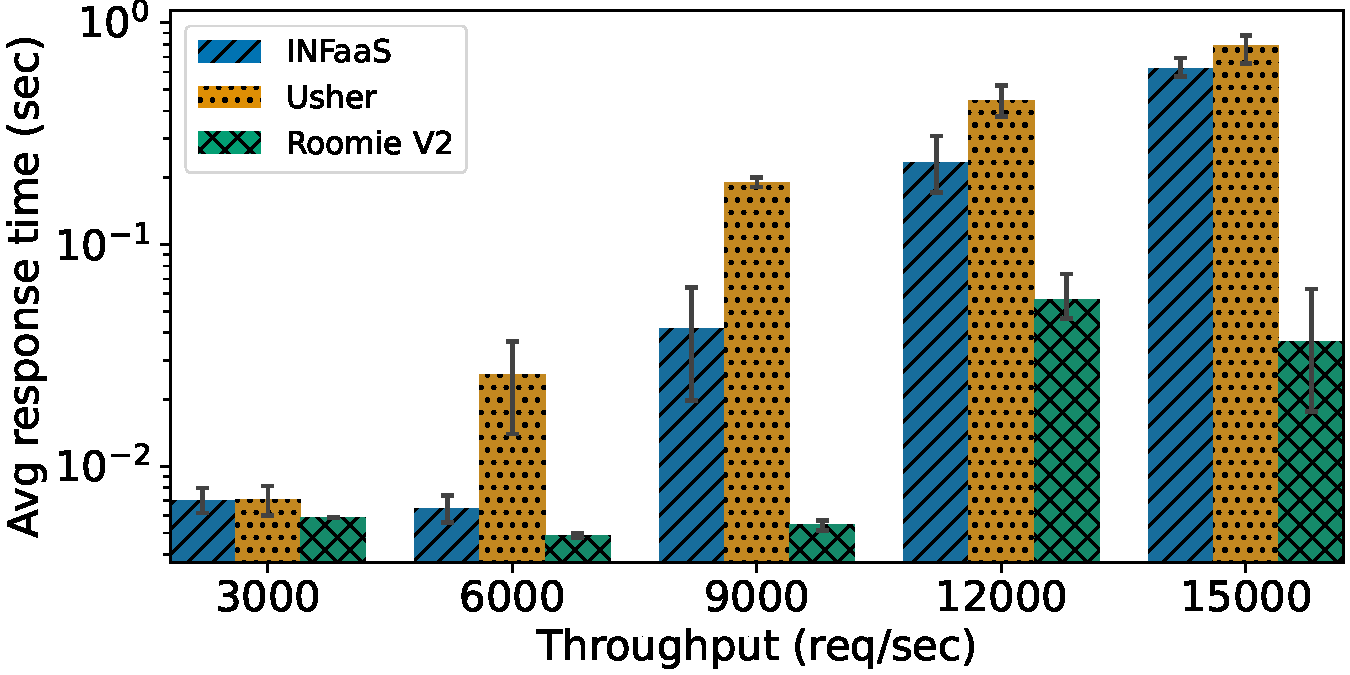
\includegraphics[width=\textwidth]{chapters/roomie/images/NvidiaA100/twitter-all-models/response_time.pdf}
		\subcaption{Response time.}
	\end{subfigure}
	\hfill
	\begin{subfigure}[b]{0.45\textwidth}
		\centering
		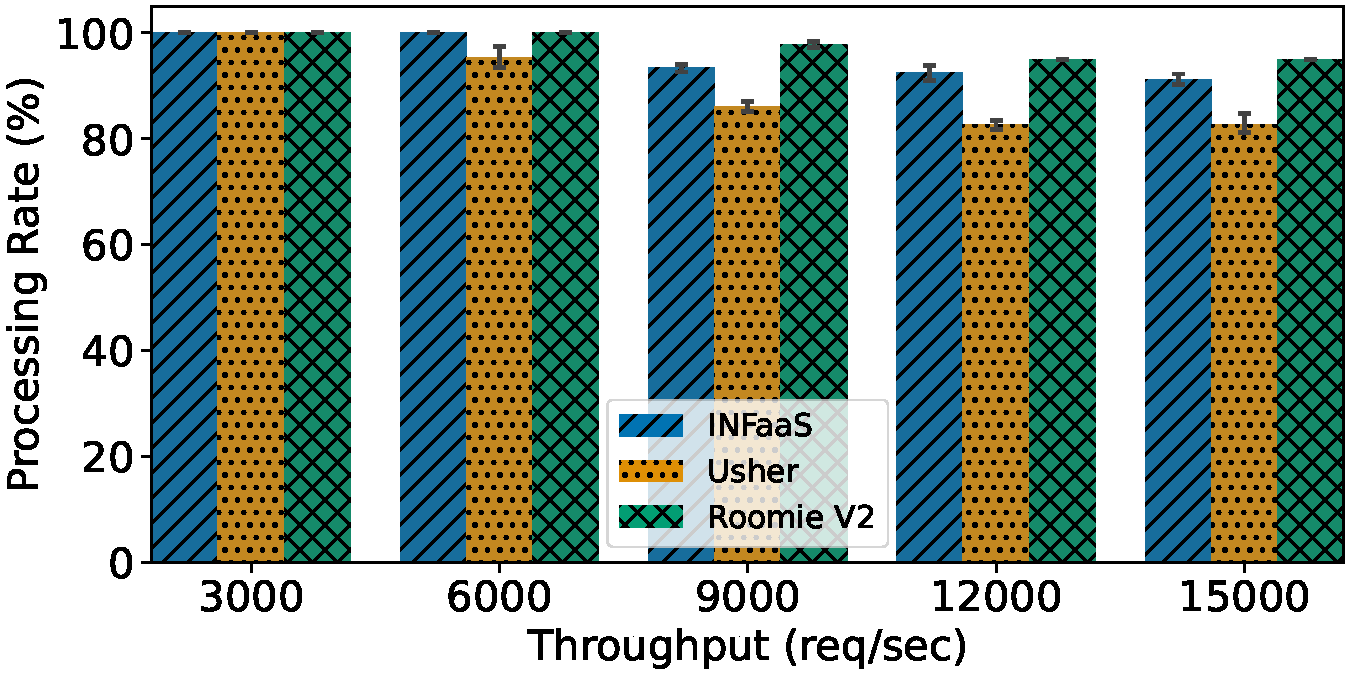
\includegraphics[width=\textwidth]{chapters/roomie/images/NvidiaA100/twitter-all-models/normalized.pdf}
		\subcaption{Processing rate.}
	\end{subfigure}
	
	\vspace{0.5cm} % Space between the rows
	
	\begin{subfigure}[b]{0.45\textwidth}
		\centering
		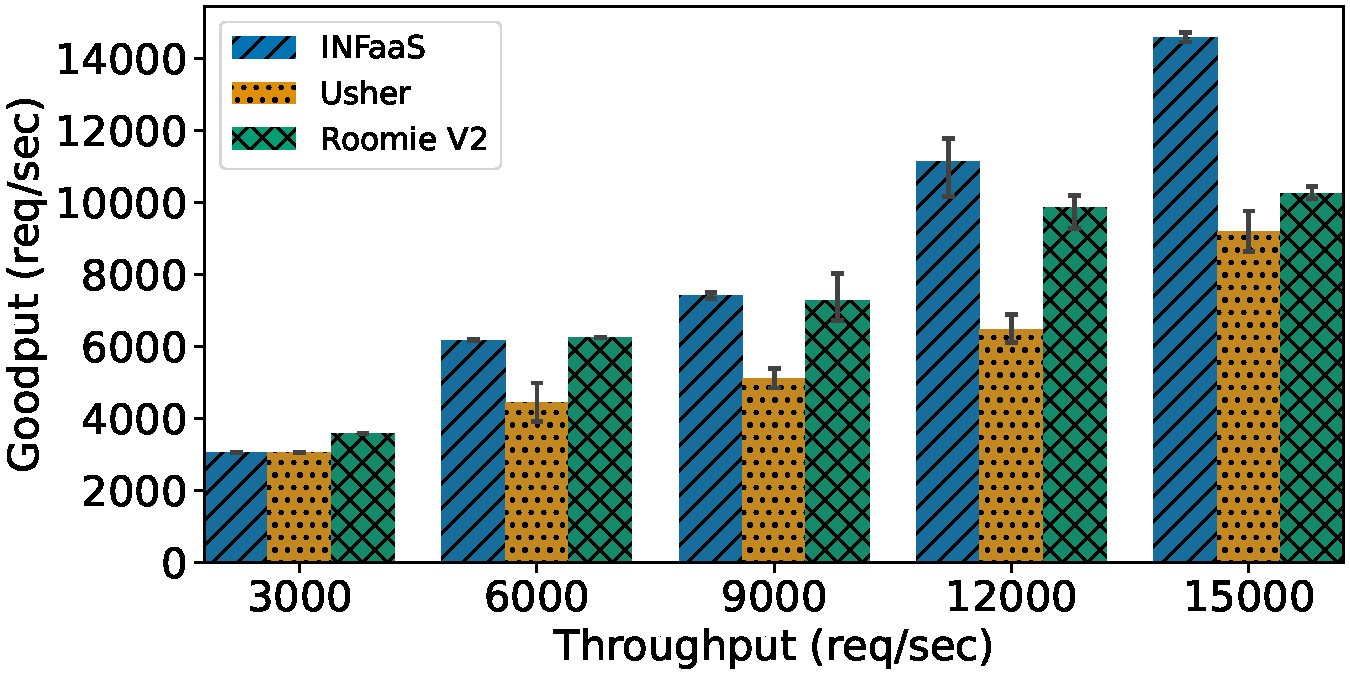
\includegraphics[width=\textwidth]{chapters/roomie/images/NvidiaA100/twitter-all-models/goodput.pdf}
		\subcaption{Goodput.}
	\end{subfigure}
	\hfill
	\begin{subfigure}[b]{0.45\textwidth}
		\centering
		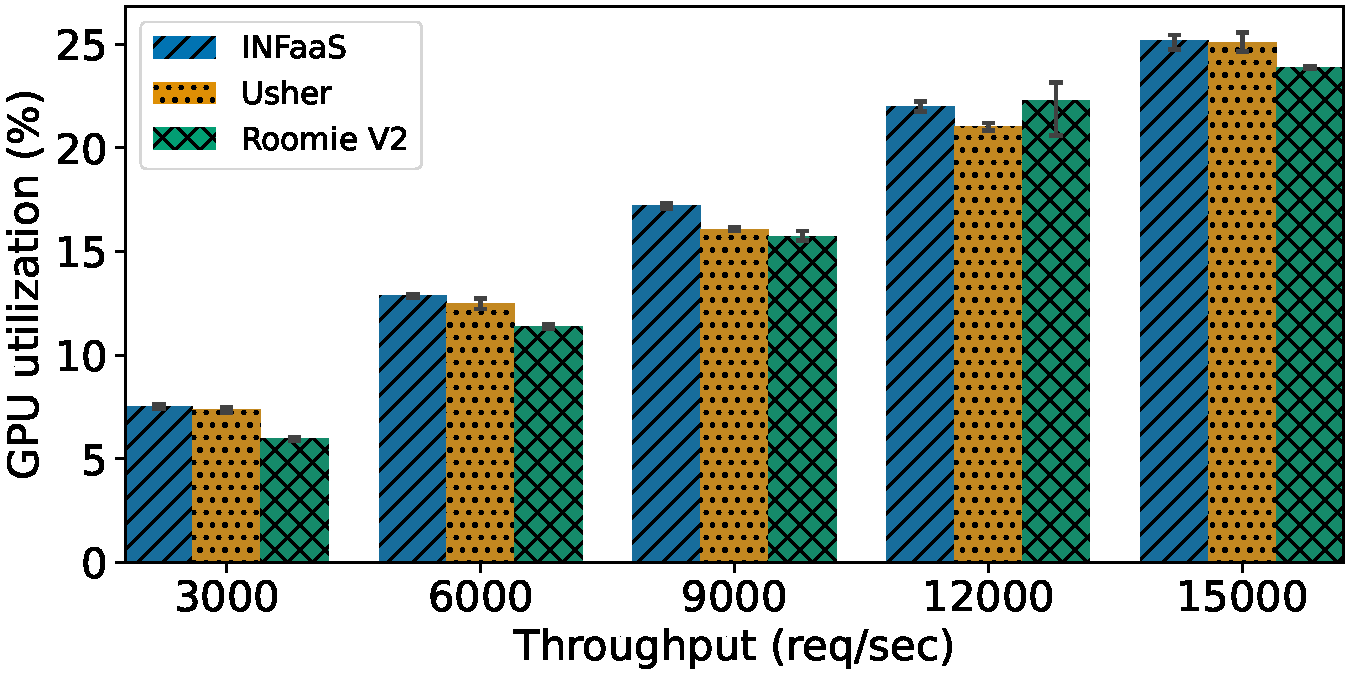
\includegraphics[width=\textwidth]{chapters/roomie/images/NvidiaA100/twitter-all-models/gpu_utilization.pdf}
		\subcaption{\acrshort{gpu} utilization}
	\end{subfigure}
	
	\caption{\roomie{} achieves up to 17$\times$ faster response times while delivering similar processing rates in a cloud-based evaluation using the Twitter dataset, outperforming INFaaS and Usher under high workload conditions.}
	\label{fig:NvidiaA100/twitter-all-models}
\end{figure}


\Cref{fig:NvidiaA100/twitter-all-models} shows the performance results obtained from the Twitter database. Under low workload conditions, all approaches showed comparable response times. However, as the workload increased, significant performance disparities emerged. Notably,~\roomie{} achieved response times up to 17× faster than rival solutions and maintained a processing rate above 97\%. In contrast, Usher's strategy of co-locating large models with lightweight models failed to deliver satisfactory performance under high load, resulting in increased latency and reduced goodput. INFaaS, which scales \acrshort{dnn}s on workers already hosting a copy, showed moderate goodput performance. However, this approach is agnostic to model interference, leading to latency increases of up to 17× and a decline in processing rate.

Interestingly, despite low \acrshort{gpu} utilization across all approaches, we observe a significant increase in response time as workload intensifies. This counterintuitive behavior can be attributed to the saturation of large models, which become unable to keep pace with incoming queries. As these models reach their computational limits, they begin to queue requests, leading to latency explosions—even though the \acrshort{gpu} itself remains underutilized. Additionally, interference between co-located models can further degrade responsiveness, compounding delays without a corresponding rise in \acrshort{gpu} activity. One potential mitigation strategy is to increase batch sizes, which can improve utilization by amortizing overhead across multiple queries. However, this approach introduces a trade-off: larger batches may inflate response times, making it unsuitable for latency-sensitive applications. These findings underscore the need for deployment strategies that go beyond raw utilization metrics and account for model saturation dynamics and cross-model interference.


\paragraph{Evaluation on synthetic dataset.}

\begin{figure}[h!]
	\centering
	\begin{subfigure}[b]{0.45\textwidth}
		\centering
		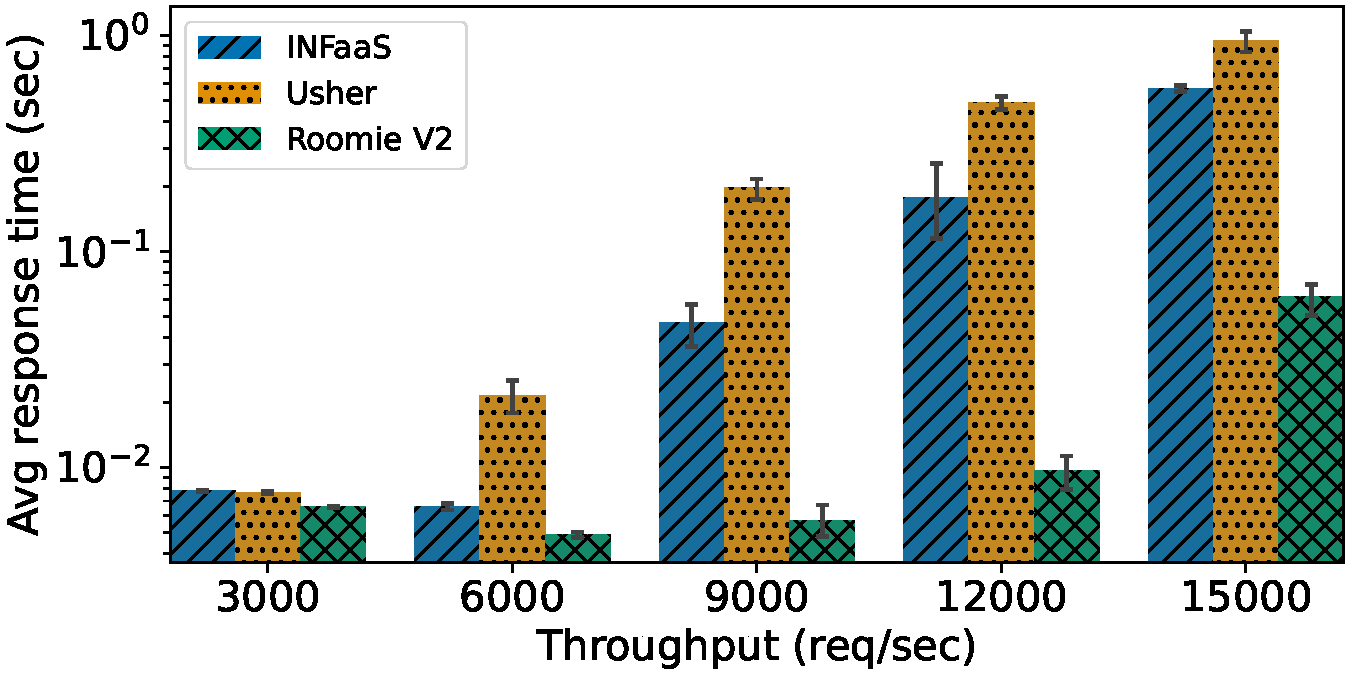
\includegraphics[width=\textwidth]{chapters/roomie/images/NvidiaA100/synthetic-all-models/response_time.pdf}
		\subcaption{Response time.}
		\label{fig:NvidiaA100/synthetic-all-models/response-time}
	\end{subfigure}
	\hfill
	\begin{subfigure}[b]{0.45\textwidth}
		\centering
		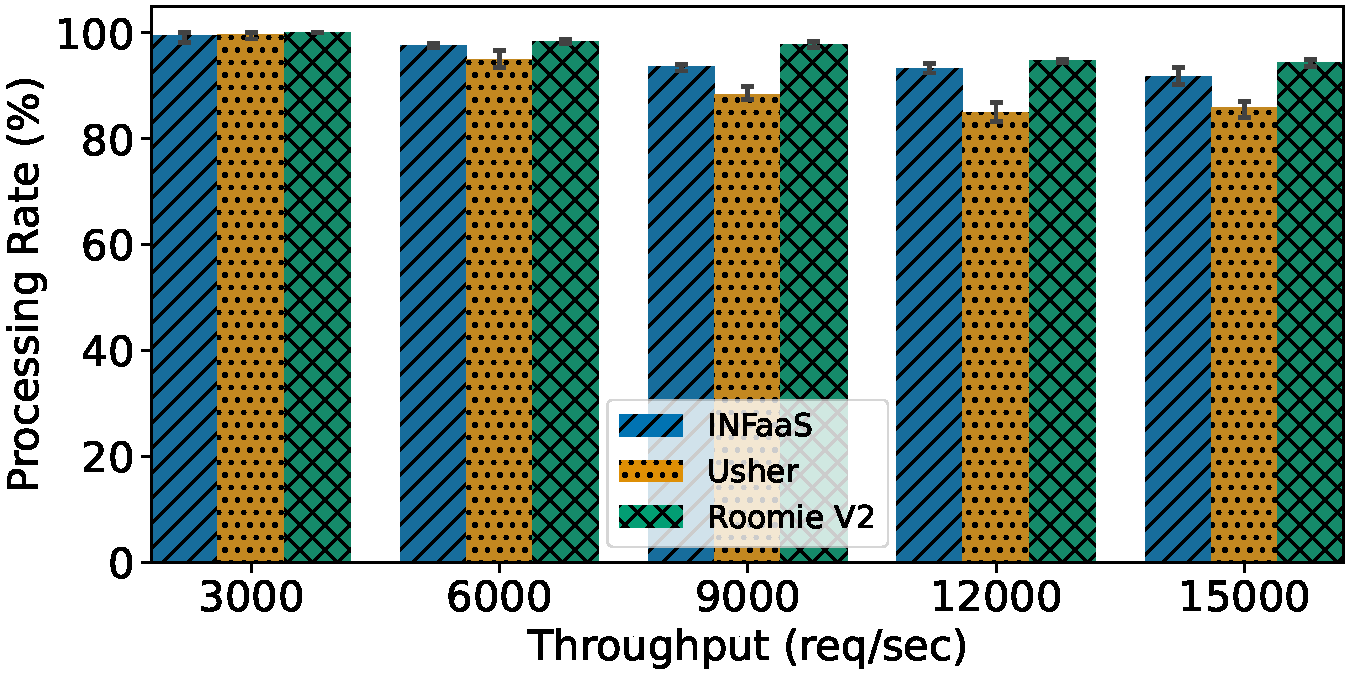
\includegraphics[width=\textwidth]{chapters/roomie/images/NvidiaA100/synthetic-all-models/normalized.pdf}
		\subcaption{Processing rate.}
	\end{subfigure}
	
	\vspace{0.5cm} % Space between the rows
	
	\begin{subfigure}[b]{0.45\textwidth}
		\centering
		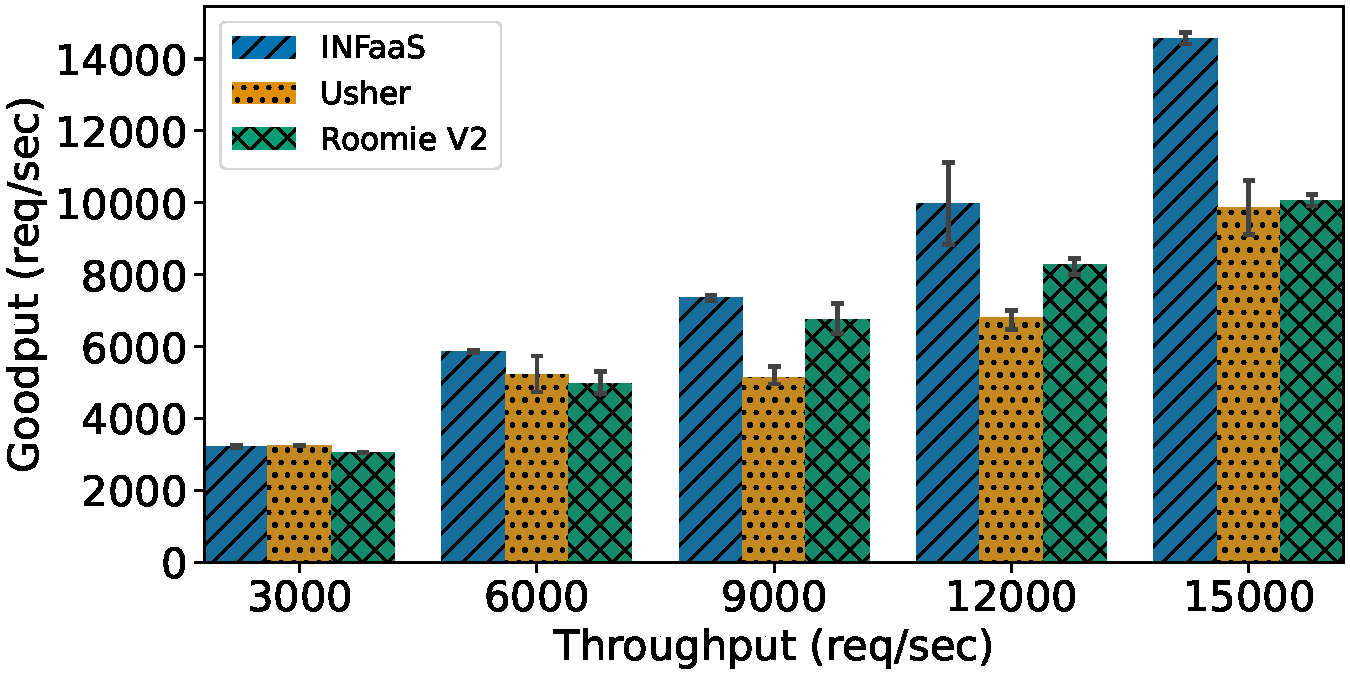
\includegraphics[width=\textwidth]{chapters/roomie/images/NvidiaA100/synthetic-all-models/goodput.pdf}
		\subcaption{Goodput.}
	\end{subfigure}
	\hfill
	\begin{subfigure}[b]{0.45\textwidth}
		\centering
		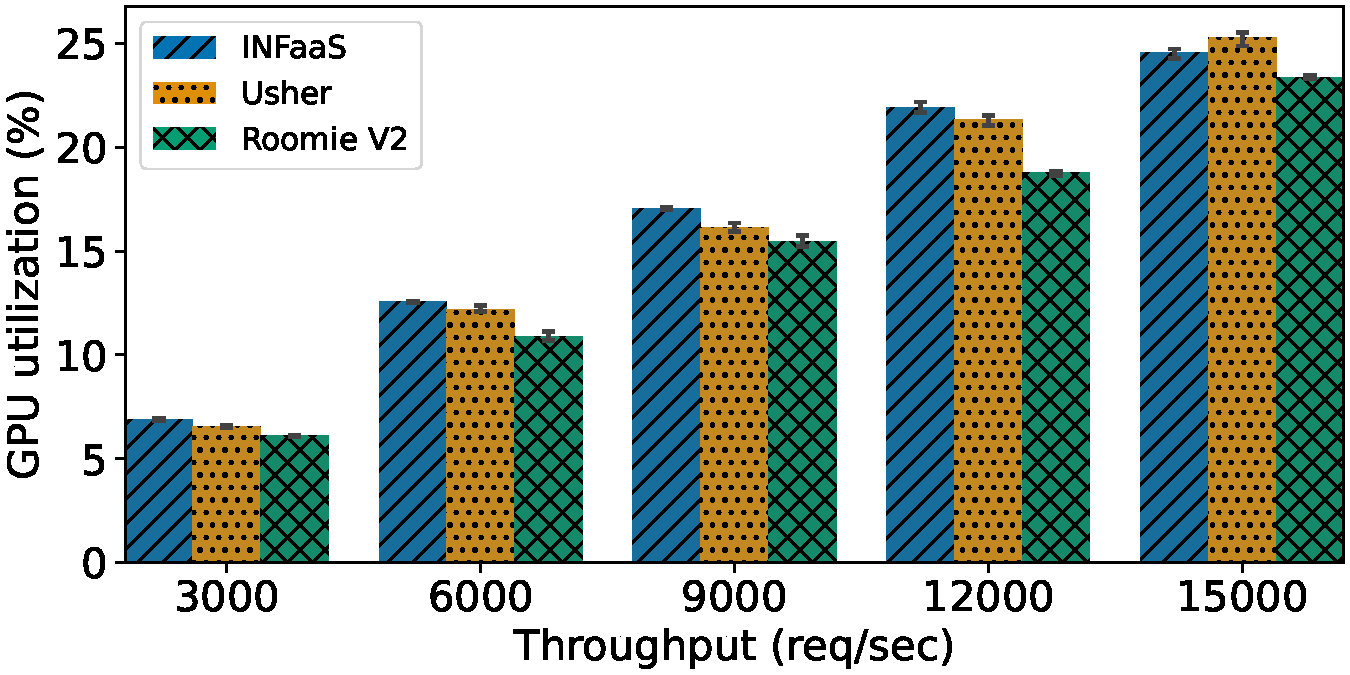
\includegraphics[width=\textwidth]{chapters/roomie/images/NvidiaA100/synthetic-all-models/gpu_utilization.pdf}
		\subcaption{\acrshort{gpu} utilization.}
	\end{subfigure}
	\caption{In cloud-based evaluation using synthetic workloads,~\roomie{} yields 9.2× faster response time and higher processing rate, confirming its deployment efficiency in controlled stress scenarios.}
	\label{fig:NvidiaA100/synthetic-all-models}
	\vspace{-3mm}
\end{figure}


\Cref{fig:NvidiaA100/synthetic-all-models/response-time} illustrates the results of the evaluation conducted with a synthetic dataset designed to emulate diverse and controlled workload scenarios.\\
The performance trends observed with the synthetic dataset closely mirrored those seen with the Twitter data.~\roomie{} consistently outperformed other deployment strategies, achieving a 9.2× reduction in response time and superior throughput and processing rates. These gains are attributed to~\roomie's intelligent model deployment and colocation strategy, which minimizes interference and maximizes resource efficiency.

Overall, across both datasets,~\roomie{} demonstrated robust performance under varying workload conditions. It consistently achieved lower response times—up to 17× faster, and higher processing rate than competing approaches, validating its effectiveness in cloud-based \acrshort{gpu} environments.



\subsection{Performance Evaluation on Edge Devices Using Jetson Xavier \acrshort{gpu}s}

To further validate our approach, we conducted a second set of experiments using a cluster of 12 Jetson Xavier \acrshort{gpu}s, representative of resource-constrained edge computing environments. As in the cloud-based evaluation, we deployed 12 models (from~\Cref{tab:dnn-models}) and tested performance using Twitter data and synthetic data, gradually increasing the workload intensity.

\paragraph{Evaluation on twitter dataset.}

\begin{figure}[h!]
	\centering
	\begin{subfigure}[b]{0.45\textwidth}
		\centering
		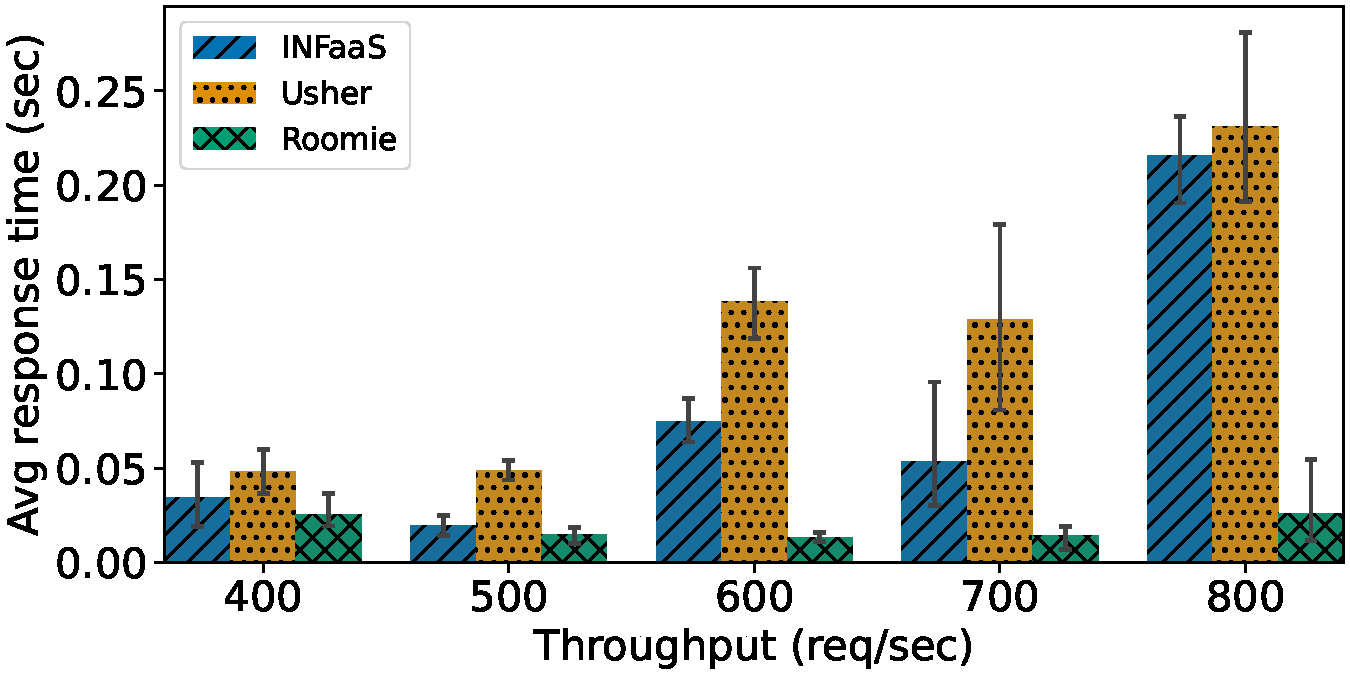
\includegraphics[width=\textwidth]{chapters/roomie/images/JetsonNano/twitter-all-models/response_time.pdf}
		\subcaption{Response time.}
	\end{subfigure}
	\hfill
	\begin{subfigure}[b]{0.45\textwidth}
		\centering
		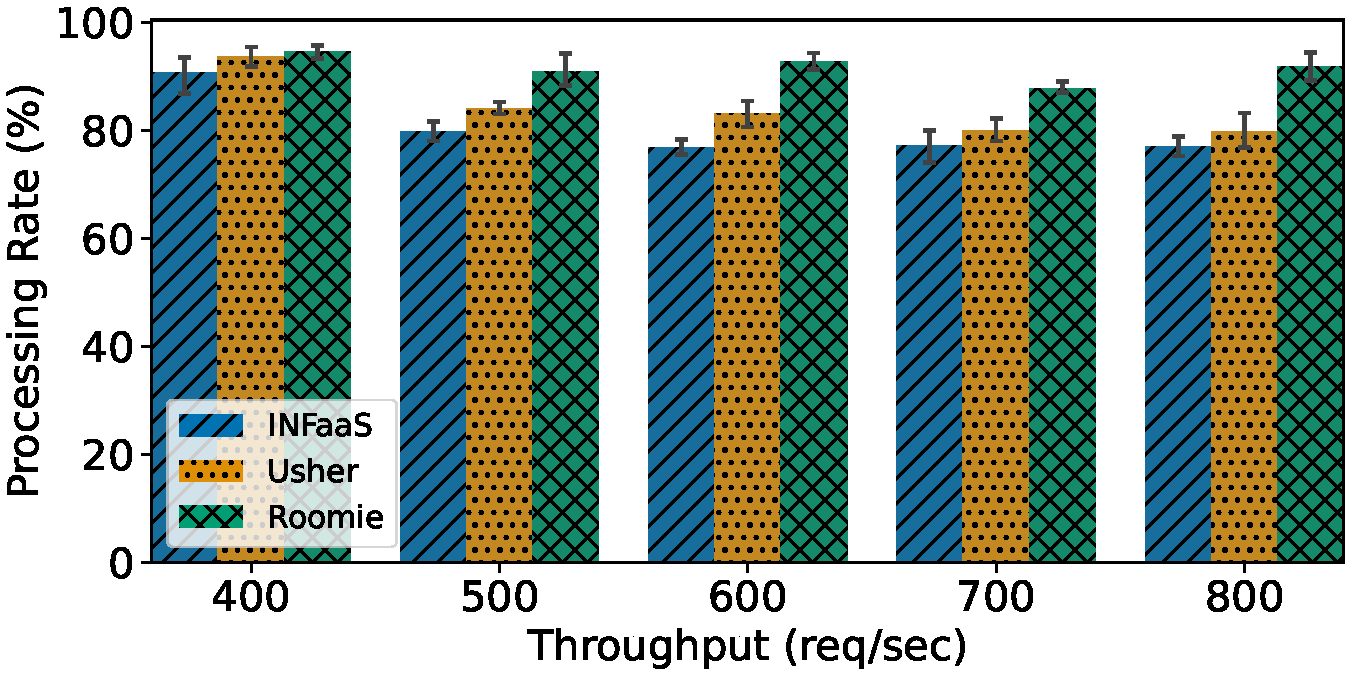
\includegraphics[width=\textwidth]{chapters/roomie/images/JetsonNano/twitter-all-models/normalized.pdf}
		\subcaption{Processing rate.}
	\end{subfigure}
	
	\vspace{0.5cm} % Space between the rows
	
	\begin{subfigure}[b]{0.45\textwidth}
		\centering
		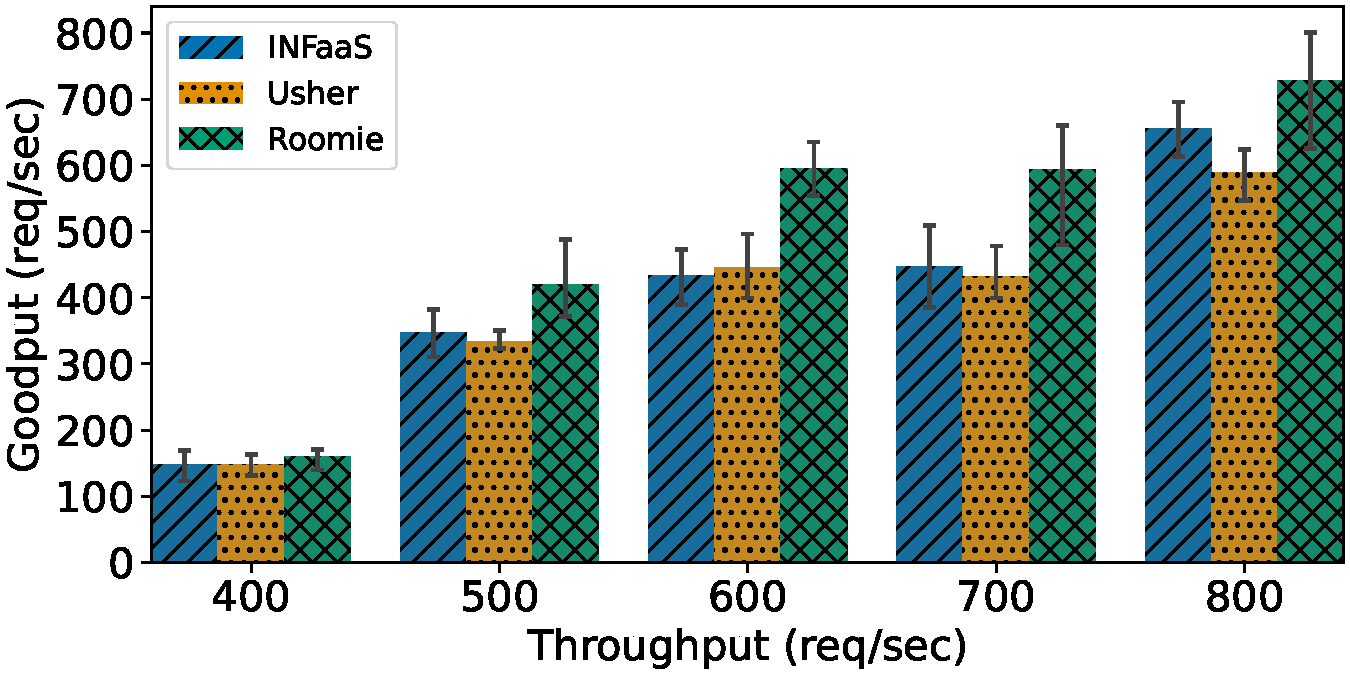
\includegraphics[width=\textwidth]{chapters/roomie/images/JetsonNano/twitter-all-models/goodput.pdf}
		\subcaption{Goodput.}
	\end{subfigure}
	\hfill
	\begin{subfigure}[b]{0.45\textwidth}
		\centering
		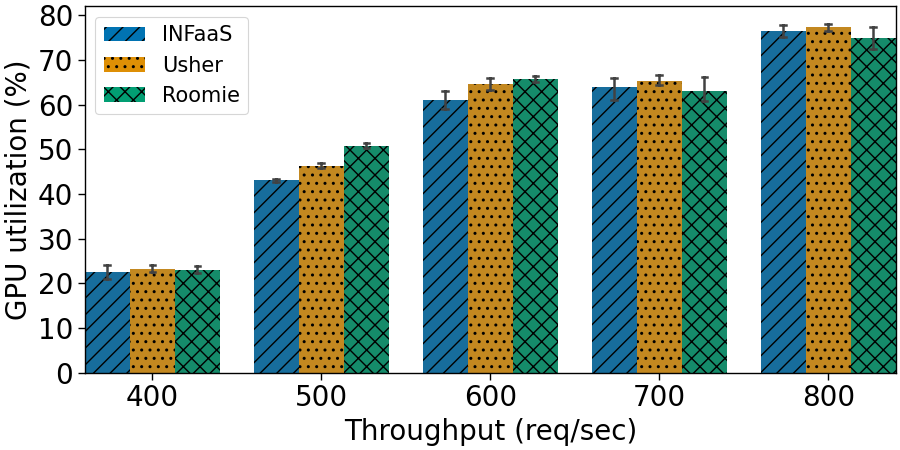
\includegraphics[width=\textwidth]{chapters/roomie/images/JetsonNano/twitter-all-models/gpu_utilization.png}
		\subcaption{\acrshort{gpu} utilization.}
	\end{subfigure}
	\caption{Edge-based evaluation on the Twitter dataset shows~\roomie{} delivering 8.3× lower latency and superior throughput on Jetson Xavier \acrshort{gpu}s, validating its proactive colocation strategy under constrained resources.}
	\label{fig:JetsonNano/twitter-all-models}
	\vspace{-3mm}
\end{figure}

The~\Cref{fig:JetsonNano/twitter-all-models} presents the results obtained with the Twitter dataset on Jetson Xavier devices. While Usher and INFaaS exhibited similar throughput levels, INFaaS achieved lower latency, whereas Usher maintained a higher processing rate.~\roomie, nevertheless, significantly outperformed both, achieving an 8.3× reduction in latency compared to INFaaS under high workload conditions. It also delivered superior throughput and processing rates due to its proactive colocation strategy.

Edge environments impose more severe constraints on model deployment due to limited computing resources and reduced scalability. In this context,~\roomie's colocation strategy offers a significant advantage, effectively balancing resource allocation and minimizing performance degradation. As workload intensity increases, \acrshort{gpu} utilization increases accordingly, reaching levels significantly higher than those seen in cloud-based configurations. This underscores the critical importance of intelligent colocation policies in edge scenarios, where resource efficiency has a direct impact on system responsiveness and throughput.

\paragraph{Evaluation on synthetic dataset.}

\begin{figure}[h!]
	\centering
	\begin{subfigure}[b]{0.45\textwidth}
		\centering
		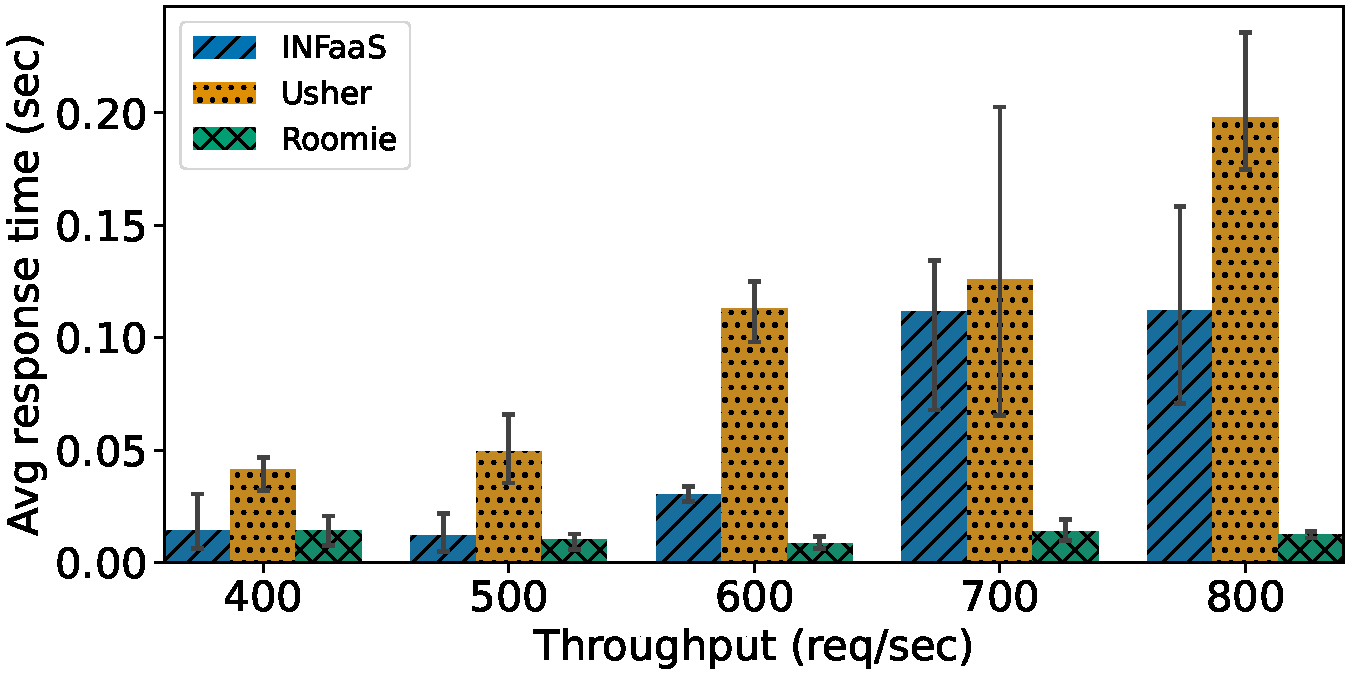
\includegraphics[width=\textwidth]{chapters/roomie/images/JetsonNano/synthetic-all-models/response_time.pdf}
		\subcaption{Response time.}
	\end{subfigure}
	\hfill
	\begin{subfigure}[b]{0.45\textwidth}
		\centering
		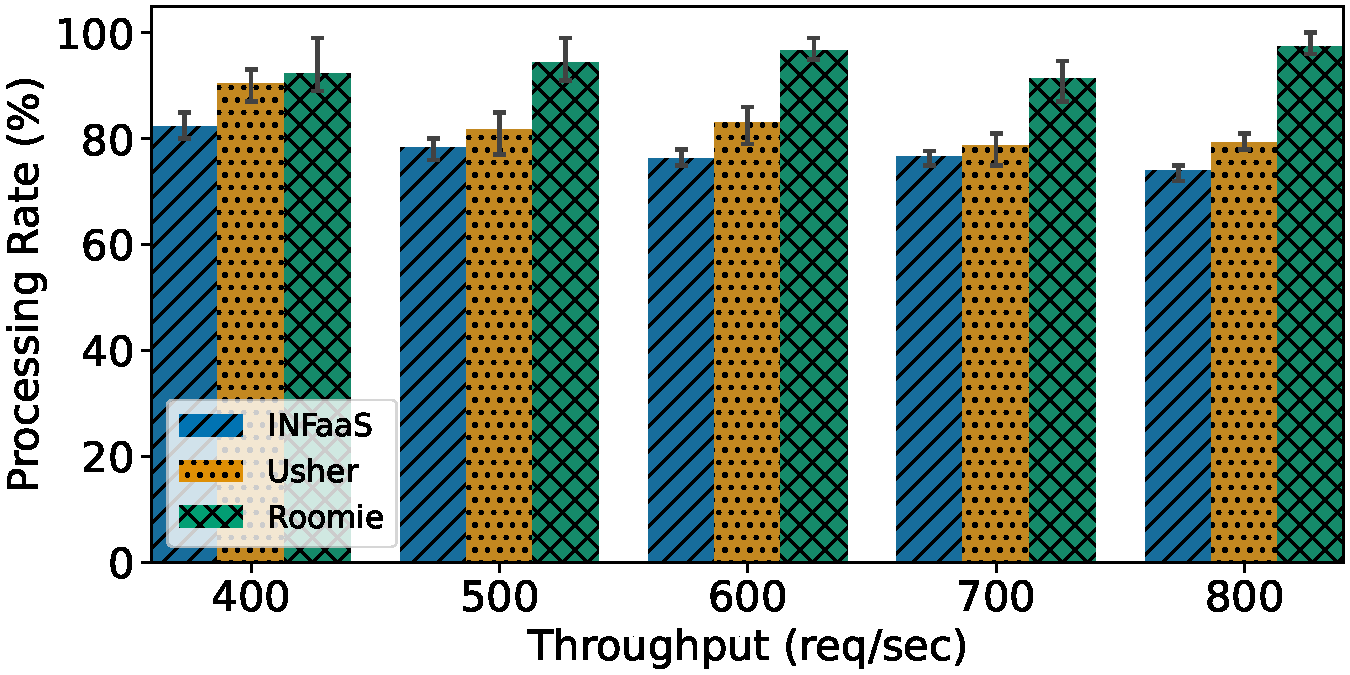
\includegraphics[width=\textwidth]{chapters/roomie/images/JetsonNano/synthetic-all-models/normalized.pdf}
		\subcaption{Processing rate.}
	\end{subfigure}
	
	\vspace{0.5cm} % Space between the rows
	
	\begin{subfigure}[b]{0.45\textwidth}
		\centering
		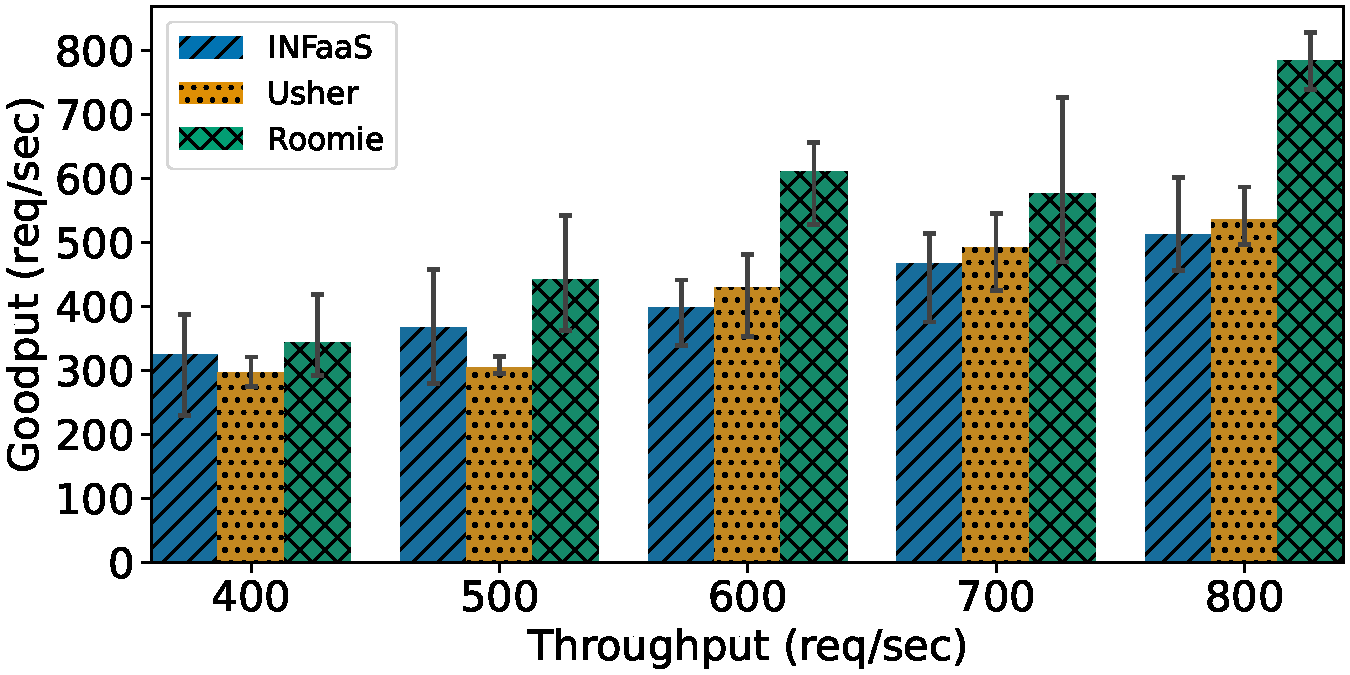
\includegraphics[width=\textwidth]{chapters/roomie/images/JetsonNano/synthetic-all-models/goodput.pdf}
		\subcaption{Goodput.}
	\end{subfigure}
	\hfill
	\begin{subfigure}[b]{0.45\textwidth}
		\centering
		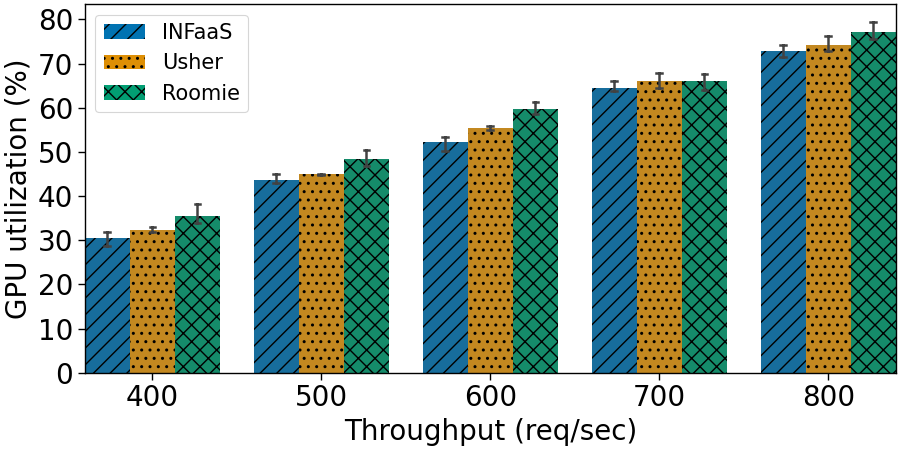
\includegraphics[width=\textwidth]{chapters/roomie/images/JetsonNano/synthetic-all-models/gpu_utilization.png}
		\subcaption{\acrshort{gpu} utilization.}
	\end{subfigure}
	\caption{Under synthetic edge evaluation,~\roomie{} sustains 9× faster response time and 1.5× higher throughput, demonstrating robust performance in resource-limited environments.}
	\label{fig:JetsonNano/synthetic-all-models}
	\vspace{-3mm}
\end{figure}

The synthetic dataset evaluation on Jetson Xavier \acrshort{gpu}s yielded consistent results with those observed on the Twitter dataset. The results are shown in~\Cref{fig:JetsonNano/synthetic-all-models}.~\roomie{} again demonstrated superior performance, achieving a 9× reduction in response time and a 1.3× increase in processing rate. Throughput was also 1.5× higher than competing approaches.

These findings confirm that~\roomie{} is the most effective \acrshort{dnn} deployment strategy in edge computing contexts where colocation is necessary and resources are limited. Its ability to maintain low latency and high throughput under constrained conditions makes it a compelling solution for real-time inference workloads.


\subsection{Evaluating~\roomie{} Deployment Accuracy Against Optimal Strategies}

\begin{figure}[t!]
	\centering
	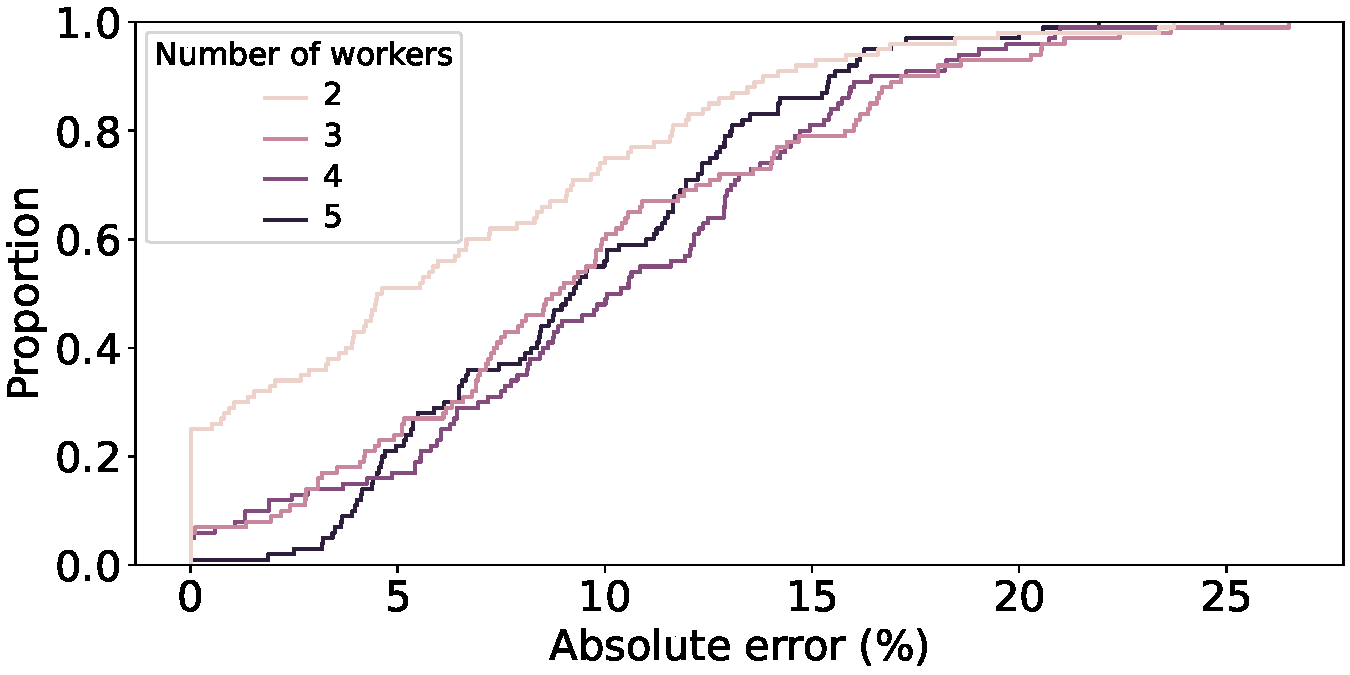
\includegraphics[width=\textwidth]{chapters/roomie/images/performance_gap_per_worker.pdf}
	\caption{Empirical CDF of~\roomie's performance gap relative to the optimal deployment strategy.}
	\label{fig:performance_gap}
\end{figure}

This section investigates the efficacy of~\roomie{} for the deployment of \acrshort{dnn}s across a varying number of workers, specifically between two and five. For each configuration, the quantity of \acrshort{dnn}s to be deployed was randomly selected from a range of two to three times the number of workers, guided by predefined options outlined in~\Cref{tab:dnn-models}. More than 100 randomized evaluations were conducted to ensure comprehensive coverage of deployment scenarios. In each evaluation, all feasible deployment permutations were thoroughly assessed to determine the configuration that resulted in the minimal average performance drop, defined as the optimal baseline. Subsequently, \roomie{} approach was applied to the same scenarios, and the absolute error between \roomie{} and optimal deployments was calculated. The cumulative distribution function (CDF) in~\Cref{fig:performance_gap} summarizes the accuracy of~\roomie{} deployment strategy for deep neural networks (\acrshort{dnn}s).

The first key observation lies in the low-error range. With two workers, 25\% of deployments fall below 0.4\% error, indicating that~\roomie{} often achieves near-optimal results in simple configurations. This sharply contrasts with higher concurrency levels, where the lower quartile rises to over 5\% for three or more workers. This shift reflects the increasing difficulty of estimating performance under competitive conditions, where profiling tools such as Nsight-Compute introduce overhead that distorts kernel execution metrics central to the modeling process.\\
The second key value is the central tendency. The median error climbs from 4\% with two workers to 10\% with four, before slightly receding with five. This peak coincides with the most pronounced modeling challenges, where pairwise colocation and reduced configuration space, used to accelerate convergence, begin to weaken. As concurrency increases,~\roomie{} must account for overlapping execution schedules and interleaved kernels, which obscure the relative timing of model completions and complicate inference behavior.\\
Third, the highest observed errors across configurations do not follow a consistent upward or downward trend, but instead fluctuate with concurrency. It rises from 13\% with two workers to 17\% with three, then drops slightly to 16\% with four and further to 15\% with five. This pattern suggests that while~\roomie{} faces its greatest challenges in intermediate configurations, it regains robustness as the system becomes more distributed. The added flexibility at higher concurrency levels appears to mitigate some of the estimation noise introduced by profiling and architectural interference.

Overall, the analysis demonstrates that~\roomie{} performs reliably under low concurrency and remains competitive even as complexity increases. Its ability to maintain bounded error across a wide range of deployment scenarios is particularly notable given the inherent challenges of performance estimation in \acrshort{gpu} environments. Profiling remains indispensable for capturing fine-grained kernel behavior, despite its overhead and distortion effects.~\roomie's design, grounded in practical strategies such as pairwise colocation and reduced configuration space, proves effective in navigating these constraints. While intermediate concurrency levels expose the limits of current modeling techniques, the overall performance remains within acceptable bounds, validating~\roomie{} as a scalable and interference-aware solution for multi-model deployment.

\label{lastpage}\section{Conclusion}\label{sec:conclusion}

\roomie{} consistently delivers high-performance deployments across both cloud and edge \acrshort{gpu} environments. In cloud settings, it achieves up to 17× lower latency and maintains over 97\% processing rate, outperforming competing strategies through interference-aware colocation and saturation resilience. On edge devices,~\roomie{} sustains its advantage with up to 9× lower response times and 1.5× higher throughput, effectively navigating resource constraints. Its heuristic maintains bounded error relative to the optimal deployment, often within 10\% even under high concurrency, despite challenges such as profiling overhead and architectural variability. These results hold across real-world and synthetic datasets, confirming~\roomie{}'s robustness and scalability. By intelligently minimizing cross-model interference and adapting to resource constraints,~\roomie{} proves to be a practical and interference-aware solution for multi-model inference in modern \acrshort{gpu} systems.


\appendix % From here onwards, chapters are numbered with letters, as is the appendix convention

\pagelayout{wide} % No margins
\addpart{Appendix}
\pagelayout{margin} % Restore margins

\setchapterstyle{lines}
\labch{appendix}

%----------------------------------------------------------------------------------------

\backmatter % Denotes the end of the main document content
\setchapterstyle{plain} % Output plain chapters from this point onwards

%----------------------------------------------------------------------------------------
%	BIBLIOGRAPHY
%----------------------------------------------------------------------------------------

% The bibliography needs to be compiled with biber using your LaTeX editor, or on the command line with 'biber main' from the template directory

\defbibnote{bibnote}{Here are the references in citation order.\par\bigskip} % Prepend this text to the bibliography
\printbibliography[heading=bibintoc, title=Bibliography, prenote=bibnote] % Add the bibliography heading to the ToC, set the title of the bibliography and output the bibliography note

%----------------------------------------------------------------------------------------
%	NOMENCLATURE
%----------------------------------------------------------------------------------------

% The nomenclature needs to be compiled on the command line with 'makeindex main.nlo -s nomencl.ist -o main.nls' from the template directory

\nomenclature{$c$}{Speed of light in a vacuum inertial frame}
\nomenclature{$h$}{Planck constant}

\renewcommand{\nomname}{Notation} % Rename the default 'Nomenclature'
\renewcommand{\nompreamble}{The next list describes several symbols that will be later used within the body of the document.} % Prepend this text to the nomenclature

\printnomenclature % Output the nomenclature

%----------------------------------------------------------------------------------------
%	GREEK ALPHABET
% 	Originally from https://gitlab.com/jim.hefferon/linear-algebra
%----------------------------------------------------------------------------------------

\vspace{1cm}

{\usekomafont{chapter}Greek Letters with Pronunciations} \\[2ex]
\begin{center}
	\newcommand{\pronounced}[1]{\hspace*{.2em}\small\textit{#1}}
	\begin{tabular}{l l @{\hspace*{3em}} l l}
		\toprule
		Character & Name & Character & Name \\ 
		\midrule
		$\alpha$ & alpha \pronounced{AL-fuh} & $\nu$ & nu \pronounced{NEW} \\
		$\beta$ & beta \pronounced{BAY-tuh} & $\xi$, $\Xi$ & xi \pronounced{KSIGH} \\ 
		$\gamma$, $\Gamma$ & gamma \pronounced{GAM-muh} & o & omicron \pronounced{OM-uh-CRON} \\
		$\delta$, $\Delta$ & delta \pronounced{DEL-tuh} & $\pi$, $\Pi$ & pi \pronounced{PIE} \\
		$\epsilon$ & epsilon \pronounced{EP-suh-lon} & $\rho$ & rho \pronounced{ROW} \\
		$\zeta$ & zeta \pronounced{ZAY-tuh} & $\sigma$, $\Sigma$ & sigma \pronounced{SIG-muh} \\
		$\eta$ & eta \pronounced{AY-tuh} & $\tau$ & tau \pronounced{TOW (as in cow)} \\
		$\theta$, $\Theta$ & theta \pronounced{THAY-tuh} & $\upsilon$, $\Upsilon$ & upsilon \pronounced{OOP-suh-LON} \\
		$\iota$ & iota \pronounced{eye-OH-tuh} & $\phi$, $\Phi$ & phi \pronounced{FEE, or FI (as in hi)} \\
		$\kappa$ & kappa \pronounced{KAP-uh} & $\chi$ & chi \pronounced{KI (as in hi)} \\
		$\lambda$, $\Lambda$ & lambda \pronounced{LAM-duh} & $\psi$, $\Psi$ & psi \pronounced{SIGH, or PSIGH} \\
		$\mu$ & mu \pronounced{MEW} & $\omega$, $\Omega$ & omega \pronounced{oh-MAY-guh} \\
		\bottomrule
	\end{tabular} \\[1.5ex]
	Capitals shown are the ones that differ from Roman capitals.
\end{center}

%----------------------------------------------------------------------------------------
%	GLOSSARY
%----------------------------------------------------------------------------------------

% The glossary needs to be compiled on the command line with 'makeglossaries main' from the template directory

\setglossarystyle{listgroup} % Set the style of the glossary (see https://en.wikibooks.org/wiki/LaTeX/Glossary for a reference)
\printglossary[title=Special Terms, toctitle=List of Terms] % Output the glossary, 'title' is the chapter heading for the glossary, toctitle is the table of contents heading

%----------------------------------------------------------------------------------------
%	INDEX
%----------------------------------------------------------------------------------------

% The index needs to be compiled on the command line with 'makeindex main' from the template directory

\printindex % Output the index

%----------------------------------------------------------------------------------------
%	BACK COVER
%----------------------------------------------------------------------------------------

% If you have a PDF/image file that you want to use as a back cover, uncomment the following lines

%\clearpage
%\thispagestyle{empty}
%\null%
%\clearpage
%\includepdf{cover-back.pdf}

%----------------------------------------------------------------------------------------

\end{document}
